\documentclass[12pt,a4paper]{article}
\usepackage[utf8]{inputenc}
\usepackage{vietnam}
\usepackage[left=3cm, right=2cm, top=2.5cm, bottom=2.5cm]{geometry}
\usepackage{amsmath}
%\usepackage{asmfonts}
\usepackage{float}
\usepackage{amssymb} 
\usepackage{graphicx} % thư viện hiển thị hình ảnh
\usepackage[hidelinks, unicode]{hyperref} % thư viện link tới chướng
\usepackage{caption} % thư viện đặt caption
\usepackage[table]{xcolor} % thư viện hiển thị màu cho bảng
%\usepackage{indentfirst}
\usepackage{mathptmx}
\renewcommand{\baselinestretch}{1.5}

\newcommand{\subsubsubsection}[1]{\paragraph{#1}\mbox{}\\}

\setcounter{secnumdepth}{4}
\setcounter{tocdepth}{4}
\geometry{letterpaper}
\title{\textbf{ĐỒ ÁN MÔN HỌC}}
\author{Luong Khanh Loc\\Bui Trong Nghia}

\begin{document}

\pagenumbering{gobble}
%\thispagestyle{empty}
\clearpage

\pdfbookmark{\contentsname}{content}
\maketitle
\newpage
\begin{center}
	\centering
	\text{ĐỒ ÁN ĐƯỢC HOÀN THÀNH TẠI}\\ 
	\textbf{TRƯỜNG ĐẠI HỌC DẦU KHÍ VIỆT NAM}
\end{center}
Người hướng dẫn chính:..................................................\\
(\textit{Ghi rõ họ, tên, học hàm, học vị})\\
\newline
Người hướng dẫn phụ (\textit{Nếu có}):......................................\\
(\textit{Ghi rõ họ, tên, học hàm, học vị})\\
\newline
Người chấm phản biện:....................................................\\
(\textit{Ghi rõ họ, tên, học hàm, học vị})\\
\newline
\newline
\newline
\newline
\newline
\newline
Đồ án được bảo vệ tại:
\begin{center}
	\centering
	\textbf{HỘI ĐỒNG CHẤM ĐỒ ÁN MÔN HỌC}\\
	\textbf{TRƯỜNG ĐẠI HỌC DẦU KHÍ VIỆT NAM}\\
	Ngày .... tháng .... năm ....
\end{center}
\newpage
\begin{table}[h]
\centering
\label{my-label}
\begin{tabular}{cc}
 \textbf{TRƯỜNG ĐẠI HỌC DẦU KHÍ VIỆT NAM} & \textbf{CỘNG HÒA XÃ HỘI CHỦ NGHĨA VIỆT NAM} \\
 \underline{\textbf{KHOA DẦU KHÍ}}& \underline{\textbf{ĐỘC LẬP - TỰ DO - HẠNH PHÚC}}
\end{tabular}
\end{table}
\begin{center}
	\centering
	\textbf{NHIỆM VỤ ĐỒ ÁN MÔN HỌC}
\end{center}

\textbf{Họ và tên SV:} \textit{Lương Khánh Lộc} \hspace{98pt} \textbf{MSSV:} \textit{04PET110009} 

\hspace{68pt} \textit{Bùi Trọng Nghĩa} \hspace{107pt} \textbf{MSSV:} \textit{04PET110011}

\hspace{68pt} \textit{Vũ Thành Hiếu} \hspace{114pt} \textbf{MSSV:} \textit{04PET110007} \par
\textbf{Ngành:} \textit{Kỹ thuật dầu khí} \hspace{138pt} \textbf{Lớp:} \textit{K4KKT}
\begin{enumerate}
	\item Tên đồ án môn học: \textit{Nghiên cứu và ứng dụng công nghệ khoan dưới cân bằng tại Thềm lục địa Việt Nam.}
	\item Nhiệm vụ(Nội dung đồ án):\\
	Chương 1: Mở đầu\\
	Chương 2: Cơ sở lý thuyết\\
	Chương 3: Các kỹ thuật khoan trong phương pháp khoan dưới cân bằng\\
	Chương 4: Các vấn đề thường gặp trong khoan dưới cân bằng\\
	Chương 5: Kiểm soát các thông số trong quá trình khoan dưới cân bằng\\
	Chương 6: Kết luận và kiến nghị.
	\item Ngày giao đồ án môn học: \textit{22/9/2017}
	\item Ngày hoàn thành đồ án môn học: \textit{10/12/2017}
	\item Họ và tên người hướng dẫn: \textit{Ths. Bùi Tử An} và \textit{KS. Phan Trọng Huân}.	
\end{enumerate}
\begin{flushright}
Bà Rịa - Vũng Tàu, ngày \ldots tháng \ldots năm \ldots
\end{flushright}
\textbf{HIỆU TRƯỞNG} \hspace{30pt} \textbf{TRƯỞNG PHÒNG ĐÀO TẠO} \hspace{30pt} \textbf{NGƯỜI HƯỚNG DẪN}\\
(Ký, ghi rõ họ tên) \hspace{60pt} (Ký, ghi rõ họ tên) \hspace{80pt} (Ký, ghi rõ họ tên)
%\clearpage
\newpage
\begin{table}[h]
\centering
\label{my-label}
\begin{tabular}{cc}
 \textbf{TRƯỜNG ĐẠI HỌC DẦU KHÍ VIỆT NAM} & \textbf{CỘNG HÒA XÃ HỘI CHỦ NGHĨA VIỆT NAM} \\
 \underline{\textbf{KHOA DẦU KHÍ}}& \underline{\textbf{ĐỘC LẬP - TỰ DO - HẠNH PHÚC}}
\end{tabular}
\end{table}
\begin{center}
	\centering
	\textbf{PHIẾU NHẬN XÉT ĐỒ ÁN MÔN HỌC}\\
	(Mẫu dành cho người hướng dẫn)
\end{center}
\textbf{Tên đề tài:} Nghiên cứu và ứng dụng công nghệ khoan dưới cân bằng tại Thềm lục địa Việt Nam.\\
\textbf{Họ và tên người hướng dẫn:} \textit{Ths. Bùi Tử An} và \textit{KS. Phan Trọng Huân}.

\textbf{Họ và tên SV:} \textit{Lương Khánh Lộc} \hspace{98pt} \textbf{MSSV:} \textit{04PET110009} 

\hspace{68pt} \textit{Bùi Trọng Nghĩa} \hspace{107pt} \textbf{MSSV:} \textit{04PET110011}

\hspace{68pt} \textit{Vũ Thành Hiếu} \hspace{114pt} \textbf{MSSV:} \textit{04PET110007} \par
\textbf{Ngành:} \textit{Kỹ thuật dầu khí} \hspace{138pt} \textbf{Lớp:} \textit{K4KKT}
\begin{enumerate}
	\item Nhận xét về tinh thần và thái độ làm việc của sinh viên: .................................................\\...........................................................................................................................................\\...........................................................................................................................................
	\item Nhận xét về kết quả đạt được: .........................................................................................\\..........................................................................................................................................\\..........................................................................................................................................
	\item Những điểm thiếu xót còn tồn tại: ...................................................................................\\..........................................................................................................................................\\..........................................................................................................................................
\end{enumerate}
\begin{flushright}
Bà Rịa - Vũng Tàu, ngày \ldots tháng \ldots năm \ldots \\
\end{flushright}
\hspace{250pt} \textbf{NGƯỜI HƯỚNG DẪN}\\
\hspace*{266pt} (Ký, ghi rõ họ tên)

\newpage
\begin{table}[h]
\centering
\label{my-label}
\begin{tabular}{cc}
 \textbf{TRƯỜNG ĐẠI HỌC DẦU KHÍ VIỆT NAM} & \textbf{CỘNG HÒA XÃ HỘI CHỦ NGHĨA VIỆT NAM} \\
 \underline{\textbf{KHOA DẦU KHÍ}}& \underline{\textbf{ĐỘC LẬP - TỰ DO - HẠNH PHÚC}}
\end{tabular}
\end{table}
\begin{center}
	\centering
	\textbf{PHIẾU NHẬN XÉT ĐỒ ÁN MÔN HỌC}\\
	(Mẫu dành cho người phản biện)
\end{center}
\textbf{Tên đề tài:} Nghiên cứu và ứng dụng công nghệ khoan dưới cân bằng tại Thềm lục địa Việt Nam.\\
\textbf{Họ và tên người hướng dẫn:} \textit{Ths. Bùi Tử An} và \textit{KS. Phan Trọng Huân}.

\textbf{Họ và tên SV:} \textit{Lương Khánh Lộc} \hspace{98pt} \textbf{MSSV:} \textit{04PET110009} 

\hspace{68pt} \textit{Bùi Trọng Nghĩa} \hspace{107pt} \textbf{MSSV:} \textit{04PET110011}

\hspace{68pt} \textit{Vũ Thành Hiếu} \hspace{114pt} \textbf{MSSV:} \textit{04PET110007} \par
\textbf{Ngành:} \textit{Kỹ thuật dầu khí} \hspace{138pt} \textbf{Lớp:} \textit{K4KKT}
\\ \textbf{Phần nhận xét:}
\begin{enumerate}
	\item Về hình thức và kết cấu đồ án môn học: ........................................................................\\........................................................................................................................................
	\item Về nội dung: ..................................................................................................................\\........................................................................................................................................\\........................................................................................................................................\\........................................................................................................................................\\........................................................................................................................................
\end{enumerate}
\textbf{Điểm:}....................................................(Ghi bằng chữ)
\begin{flushright}
Bà Rịa - Vũng Tàu, ngày \ldots tháng \ldots năm \ldots \\
\end{flushright}
\hspace{260pt} \textbf{NGƯỜI PHẢN BIỆN}\\
\hspace*{273pt} (Ký, ghi rõ họ tên)
\newpage
\begin{center}
	\centering
	\textbf{LỜI CAM KẾT}
	%\section*{\textbf{LỜI CAM KẾT}}
	\addcontentsline{toc}{section}{LỜI CAM KẾT}
\end{center}
Chúng tôi xin cam đoan những kết quả nghiên cứu được trình bày trong đồ án này là hoàn toàn trung thực, không vi phạm bất cứ điều gì trong luật sở hữu trí tuệ và pháp luật Việt Nam. Nếu sai, chúng tôi sẽ hoàn toàn chịu trách nhiệm trước pháp luật.\\
\hspace*{250pt} \textbf{ĐẠI DIỆN TÁC GIẢ ĐỒ ÁN}\\
\hspace*{280pt} (Ký, ghi rõ họ tên)
\newline
\newline
\hspace*{282pt} \textit{Lương Khánh Lộc}


\clearpage
%\newpage

\pagenumbering{roman}
\thispagestyle{empty}
%\clearpage

\begin{center}
	\centering
	\textbf{LỜI CẢM ƠN}
	%\section*{\textbf{LỜI CẢM ƠN}}
	\addcontentsline{toc}{section}{LỜI CẢM ƠN}
\end{center}
Với lòng biết ơn sâu sắc nhất, nhóm em xin gửi đến quý Thầy Cô ở khoa Dầu Khí –
trường Đại Học Dầu Khí Việt Nam, không những dùng tri thức và tâm huyết của mình để truyền đạt vốn kiến thức quý báu cho chúng em trong suốt thời gian học tập tại trường mà còn tạo điều kiện và luôn ủng hộ nhóm em trong quá trình nghiên cứu hoàn thiện đồ án của nhóm. \\
Đồng thời chúng em xin gửi lời cám ơn chân thành đến thầy \textbf{Bùi Tử An} và anh \textbf{Phan Trọng Huân} đã đồng ý trở thành những người trực tiếp hướng dẫn, đưa ra gợi ý và kịp thời chỉ ra những sai sót cho chúng em trong suốt thời gian hoàn thiện đồ án.\\
Qua quá trình hoàn thiện đồ án, nhóm đã có nhiều cơ hội với những kiến thức mới đồng thời cũng cố và vận dụng những kiến thức chuyên ngành vào thực tế, rèn luyện được kĩ năng nghiên cứu thực tế bổ ích từ thầy \textbf{Bùi Tử An} và anh \textbf{Phan Trọng Huân}.\\
Do mới bước đầu tiếp cận nghiên cứu đồ án cùng với lượng kiến thức còn hạn chế nên kết quả hoàn thiện còn nhiều thiếu sót. Kính mong quý Thầy Cô đóng góp thêm ý kiến để những đồ án tiếp theo nhóm em có thể đạt kết quả tốt hơn và có thể hoàn thiện được bản thân mình hơn.
\begin{flushright}
Nhóm chúng em xin chân thành cảm ơn!
\end{flushright}
\newpage
\tableofcontents

\listoftables
\addcontentsline{toc}{section}{Danh sách bảng}

\newpage
\listoffigures
\addcontentsline{toc}{section}{Danh sách hình}

\newpage
%\textbf{Danh pháp}
\section*{\textbf{Danh pháp}}
\addcontentsline{toc}{section}{Danh pháp}
	\begin{enumerate}
		\item[] UBD = Underbalanced Drilling
		\item[] LWD = Logging While Drilling
		\item[] MWD = Measurement While Drilling
		\item[] PWD = Pressure While Drilling
		\item[] ECD = Equivalent Circulating Density
		\item[] MPD = Managed Pressure Drilling
		\item[] ROP = Rate of Penetration 
 		\item[] RCD = Rotating Control Devices
		\item[] NPT = Non-Prodctive Time
		\item[] BOP = Blow-out Preventor
		\item[] WHP = Wellhead Pressure
		\item[] NRV = Non-Return Valve
		\item[] BHA = Bottom-hole Assembly
		\item[] WOB = Weight On Bit
		\item[] BHCP = Bottom-hole Circulating Pressure
		\item[] MW = Mud Weight
		\item[] OBFDF = Oil-based Foam Drilling Fluid
		\item[] CBHP = Constant Bottom-hole Pressure
		\item[] CCS = Continuous Circulating System
 		\item[] DAPC = Dynamic Anular Pressure Control
		\item[] PMCD = Pressuried Mud Cap Drilling
		\item[] LRRS = Low Riser Return System
		\item[] DC = Dual Gredient
		\item[] ECDRT = Equivalent Circulating Density Reduction Tools
	 	\item[] HSE = Health, Safety and Environment
	 	\item[] IPR = Inflow Performance Relationship.
	\end{enumerate}
\clearpage
\pagenumbering{arabic}
\newpage
\section{Mở đầu}
\subsection{Giới thiệu về phương pháp khoan dưới cân bằng}
Khoan dưới cân bằng là một loại phương pháp khoan trong đó áp suất của cột dung dịch khoan được giữ nhỏ hơn áp suất vỉa dầu khí.
Phương pháp này được xem là phức tạp và tốn kém hơn rất nhiều so với phương pháp khoan truyền thống bời vì nó đòi hỏi những thiết bị, máy móc và qui trình vận hành phức tạp và đòi hỏi những kỹ thuật tiên tiến hơn.
\subsection{Mục đích nghiên cứu}
Tập trung nghiên cứu làm rõ những lợi ích và bất lợi của phương pháp khoan dưới cân bằng. Nghiên cứu các cơ sở lựa chọn kĩ thuật khoan cho phương pháp khoa dưới cân bằng và cơ sở thiết bị để có thể đưa phương pháp khoan dưới cân bằng vào vận hành. Kiểm tra, đánh giá và so sánh giữa phương pháp khoan truyền thống và phương pháp khoan dưới cân bằng. Nghiên cứu những điều kiện thuận lợi và khó khăn khi áp dụng công nghệ khoan dưới cân bằng vào công nghiệp dầu khí Việt Nam, cụ thể là ngành khoan – khai thác.

\subsection{Vấn đề nghiền cứu}
Công nghệ khoan dưới cân bằng đã được áp dụng phổ biến trên thế giới và mang lại nhiều lợi ích về kinh tế và an toàn.

\subsection{Phạm vi nghiên cứu}
Nghiên cứu cơ sở lý thuyết, những kỹ thuật được áp dụng trong phương pháp khoan dưới cân bằng, hệ dung dịch thích hợp cho hệ thống tuần hoàn dung dịch để có thể kiểm soát được áp suất trong giếng.


\section{Cơ sở lý thuyết}
\subsection{Áp suất vỉa và vỡ vỉa}
\subsubsection{Áp suất vỉa}
Áp suất vỉa là áp suất của lưu chất trong không gian rỗng của vỉa. Áp suất vỉa tại một điểm trong vỉa thường được coi là áp suất thủy tỉnh tại điểm đó hay áp suất được tạo ra bởi cột chất lỏng từ độ sâu của điểm đó tới mặt nước biển.
Áp suất vỉa thường được dự đoán bằng hai phương pháp, phương pháp thứ nhất dựa trên ứng suất của khung đá tại độ sâu D\cite{bourgoyne1991applied}:
\begin{equation}
p = \sigma_{ob}-\sigma_{z}
\end{equation}
Với p là áp suất vỉa, $\sigma_{ob}$ là ứng suất của lớp phủ trên tại độ sâu D, $\sigma_{z}$ là ứng suất của hạt rắn tại độ sâu D. Phương pháp thứ hai tính toán áp suất vỉa từ đồ thị thể hiện sự tương quan độ rỗng phụ thuộc vào độ sâu dựa trên thực nghiệm\cite{bourgoyne1991applied}.
\subsubsection{Áp suất vỡ vỉa}
Khi áp suất trong giếng lớn hơn áp suất vỉa ở một mức độ có thể gây ra nứt vỡ thành hệ, áp suất lúc đó được gọi là áp suất vỡ vỉa. Quá trình dự đoán áp suất vỉa dựa trên những tương quan thực nghiệm bao gồm: phương trình Hubbert – Willis, tương quan Mathews – Kelly, tương quan Pennebaker, tương quan Eaton,  phương trình Christman và tương quan MacPhersin – Berry\cite{bourgoyne1991applied}.
Theo Hubbert – Willis, để áp suất giếng nhỏ nhất có thể mở rộng được những nứt nẻ đã có sẵn, áp suất phải vượt qua được ứng suất chính nhỏ nhất:
\begin{equation}
p_{ff} = \sigma_{min}+p_{f}
\end{equation}
Tuy nhiên do cấu trúc trái đất là bất đồng nhất và bất đẳng hướng nên phương trình (2) chỉ áp dụng cho lập kế hoạch khoan và thiết kế chống ống. Trong mặt phẳng nằm ngang, áp suất vỡ vỉa cần thiết sẽ là:
\begin{equation}
p_{ff} = 2\sigma_{H}+p_{f}
\end{equation}
Với  là ứng suất theo chiều ngang. Dựa vào những phân tích sử dụng tiêu chuẩn phá hủy Mohr\cite{bourgoyne1991applied}, áp suất vỡ vỉa sẽ bằng:
\begin{equation}
p_{ff} = \frac{\sigma_{z}}{3} + p_{f}
\end{equation}
Dựa vào phương trình (1) ứng suất khung đá được tính:
\begin{equation}
\sigma_{z} = \sigma_{ob}-p_{f}
\end{equation}
Như vậy, áp suất vỡ vỉa đươc tính:
\begin{equation}
p_{ff} = \frac{\sigma_{ob}+2p_{f}}{3}
\end{equation}


\subsection{Áp suất đáy giếng}
Trong điều kiện không tuần hoàn dung dịch, áp suất đáy giếng chính là áp suất thủy tỉnh của cột dung dịch:
\begin{equation}
BHP = MW\cdot D \cdot 0.052
\end{equation}
Trong trường hợp giếng đang hoạt động, dung dịch trong giếng được tuần hoàn, áp suất đáy giếng là áp suất thủy tỉnh cộng tổn thất áp suất do ma sát. Trong đó, tổn thất áp suất do ma sát, được tính theo phương trình Darcy – Weisbach\cite{bourgoyne1991applied}.


\subsection{Dung dịch khoan}
Trong quá trình thi công khoan, đặc biệt là khoan dưới cân bằng, quá trình thiết kế lựa chọn dung dịch khoan cần phải được thực hiện hoàn chỉnh và toàn diện bởi vì đây là quá trình có ảnh hưởng trực tiếp đến các thông số thuỷ lực, ổn định thành hệ và ảnh hưởng đến quá trình khai thác. Các chức năng chính của dung dịch khoan gồm có:
\begin{enumerate}
	\item Rửa sạch đáy giếng khoan và tuần hoàn mùn khoan lên bề mặt.
	\item Kiểm soát áp suất thành hệ.
	\item Duy trì sự ổn định của thành hệ
\end{enumerate}
Ngoài ra còn có một số chức năng khác là:
\begin{itemize}
	\item Giữ mùn khoan ở trạng thái lơ lửng khi khoan
	\item Giảm thiếu tác động gây tổn hại thành hệ
	\item Làm mát, bôi trơn bộ khoan cụ, hỗ trợ làm mêm đất đá
	\item Cung cấp năng lượng cho động cơ đáy
	\item Truyền dẫn thông tin địa chất
	\item Tạo điều kiện thuận lợi cho trám xi măng và hoàn thiện giếng
	\item Duy trì độ thấm của thành hệ
	\item Kiểm soát ăn mòn bộ khoan cụ và các thiết bị khác
	\item Khống chế sự xâm nhập của dầu và khí từ thành hệ vào giếng
\end{itemize}
Tỷ trọng cột dung dich khoan được xác định bằng công thức\cite{bourgoyne1991applied}:
\begin{equation}
E.C.D = M.W +\frac{P_{circ}}{0.052xTVD}
\end{equation}
\subsection{Tổn thất áp suất}

Tổn hao áp suất trong quá trình khoan là yếu tố quan trọng để tính toán công suất thuỷ lực khoan, cũng như các vấn đề về kiểm soát giếng và tính toán hiệu suất của quá trình khoan.
\\
Giống với quá trình khoan truyền thống, tổn hap áp suất trong quá trình khoan dưới cân bằng được tính bằng tổng các tổn hao áp suất qua hệ thống tuần hoàn dung dịch, các thiết bị bề mặt và tổn hao áp suất trong lòng giếng khoan.
\\
Công thức tính tổn hao áp suất của bùn khoan\cite{aadnoy2011fundamentals}:
\begin{equation}
\Delta P = \Delta P_{DP}+ \Delta P_{DC}+\Delta P_{DC/ANN}+ \Delta P_{DP/ANN} +\Delta P_{Bit}
\end{equation}
Trong đó:
\begin{itemize}
	\item $\Delta P_{DP}$ là tổn hao áp suất trong cần khoan
	\item $\Delta P_{DC}$ là tổn hao áp suất trong cần nặng
	\item $\Delta P_{DC/ANN}$ là tổn hao áp suất ngoài vành xuyển đoạn cần nặng
	\item $\Delta P_{DP/ANN}$ là tổn hao áp suất ngoài vành xuyến đoạn cần khoan
	\item $\Delta P_{Bit}$ là tổn hao áp suất tại vòi phun.
\end{itemize}
Tính toán tổn hao áp suất là một bài toán quan trọng để tiến hành lập kế hoach thi công giếng khoan và trong quá trình khoan dưới cân bằng áp suất mất mát dùng để tính toán áp suất đáy giếng, từ đó cùng với của sổ gradient áp suất vỉa và vỡ vỉa xác định kỹ thuật cho một giếng khoan cụ thể và bài toán vận hành giếng khoan.
\section{Các kỹ thuật khoan trong phương pháp khoan dưới cân bằng}
\subsection{Tổng quan}
	Trong quá trình khoan một giếng, khi gradient áp suất trong giếng được giữ nhỏ hơn gradient áp suất vỉa thì được gọi là quá trình khoan dưới cân bằng và phương pháp này khác với các phương pháp khoan truyền thống. Trong khi khoan giếng có thể dễ dàng bị ``Kick'' do áp suất dung dịch tuần hoàn dưới đáy giếng luôn nhỏ hơn áp suất vỉa. Tuy nhiên, khi sử dụng phương pháp này, tốc độ khoan được tăng lên khá nhiều đồng thời cũng tránh được hiện tượng mất dung dịch trong khi tuần hoàn. 
\subsection{Những kỹ thuật trong khoan dưới cân bằng}
	Khi khoan áp suất trong giếng nhỏ hơn áp suất trong vỉa nên dễ tạo điều kiện xảy ra hiện tượng “Kick”. Tỉ trọng dung dịch khoan, hay tỉ trọng cột dung dịch là thông số dầu tiên cần xét đến khi muốn hạn chế hiện tượng “Kick”, đồng thời tỉ trọng cũng là một thông số giúp ổn định thành giếng. Vì vậy, việc lựa chọn kĩ thuật khoan cho phương pháp khoan dưới cân bằng là cực kỳ quan trọng. Một số kĩ thuật được đưa vào thực tế như:
	\begin{itemize}
		\item Khoan bằng khí khô
		\item Khoan bằng khí nitơ
		\item Khoan bằng khí tự nhiên 
		\item Khoan bằng khí mù
		\item Khoan bằng bọt
		\item Khoan bằng bọt sánh
		\item Khoan bằng khí hóa lỏng
		\item Flow drilling
		\item Snub drilling
	\end{itemize}
\subsection{Những ưu điểm và hạn chế khi sử dụng phương pháp khoan dưới cân bằng}
	\textbf{Ưu điểm}
	\begin{itemize}
	\item Không sử dụng tác động cơ học để tạo lực đẩy cần thiết cho dung dịch đi vào thành hệ, vì vậy sẽ hạn chế được mất dung dịch trong kể cả khi khoan ở những tầng vỉa có độ thấm cao.
	\item Giảm được thiệt hại đến thành hệ do áp suất trong giếng luôn nhỏ hơn áp suất thành hệ, giúp cho việc giảm chi phí và tiết kiệm thời gian khi kích thích giếng lúc bắt đẩu khai thác. 
	\item Giúp cho việc tìm kiếm các vỉa sản phẩm dễ dàng, nhanh chóng hơn so với phương pháp khoan truyền thống.
	\item Giảm hiện tượng kẹt cần do chênh áp bởi vì không có lớp filter cake ở thành giếng.
	\item Tốc độ khoan được cải thiện hơn so với các phương pháp khoan truyền thống do áp suất ở đầu chòong khoan thấp, đồng thời cũng kéo dài tuổi thọ của chòong khoan.
	\item Cuối cùng, không cần thiết phải xử lý dung dịch khoan nguy hại vì quá trình không sử dụng các loại dung dịch khoan theo kiểu truyền thống.
	\end{itemize}
	
	\textbf{Hạn chế}
	\begin{itemize}
	\item Giá thành cao, tùy thuộc vào loại dung dịch.
	\item Việc duy trì điểm dưới áp suất cân bằng thường khá khó khăn. Không có lớp filter cake, khi áp suất đột ngột vượt lên trên mức cân bằng thường gây ra nhiều thiệt hại.
	\item Vấn đề an toàn cũng cần được xem xét cẩn thận, vì khi thực hiện khoan dưới cân bằng phải đối mặt nhiều mối nguy hiểm hơn. Cháy, nổ và owout thường dễ xảy ra trong khi khoan dưới cân bằng.
	\item Những vấn đề khác như sập thành giếng do áp suất thành hệ lớn, thiết bị dễ bị hư hại do sử dụng những hệ dung dịch phi truyền thống.
	\item Tùy thuộc vào dung dịch sử dụng có khả năng dẫn nhiệt tốt hay kém, nhưng khi giếng thường xuyên nằm trong trạng dẫn nhiệt kém sẽ gây hư hại đến thành hệ.
	\end{itemize}
\subsection{Kỹ thuật khoan khí khô}
\subsubsection{Tổng quan}
	Kỹ thuật khoan bằng khí khô\cite{rehm2013underbalanced} được sử dụng để giảm áp suất vùng đáy giếng xuống thấp nhất để có thể tăng tối đa tốc độ khoan. Với những tính chất được thiết kế, sử dụng khí khô giúp làm mát chòong khoan và làm tăng tốc độ vận chuyển mùn khoan. Khí khô không thực hiện công việc ổn định thành giếng đồng thời cũng không ngăn dòng vào từ vỉa, mục đích duy nhất sử dụng khí khô là làm tăng tốc độ khoan nhanh nhất có thể.\\
	Tuy nhiên, khoan bằng khí khô vẫn đem lại một số lợi ích nhất định ngoài việc tăng tối đa tốc độ khoan:
	\begin{itemize}
	\item{Áp suất trong giếng giảm, tránh được hiện tượng mất dung dịch trong khi tuần hoàn.}
	\item{Có thể tìm được những vỉa có tiềm năng về dầu khí nhưng bị lấp đầy bởi nước vỉa hoặc những dung dịch dùng cho khoan trên cân bằng không thể thực hiện được.}
	\item{Bảo vệ được những tầng sản phẩm nhạy cảm trong vỉa cát chặt sít, vỉa sét nén, vỉa than.}
	\end{itemize}
\subsubsection{Thiết bị khoan}
\subsubsubsection{Đầu xoay} \\
	Để có thể áp dụng kỹ thuật khoan bằng khí cần phải có một thiết bị được gọi là thiết bị kiểm soát áp suất (RCD). Trong khi vận hành khoan việc dự tính áp suất giãn nở của khí là không cần thiết vì áp suất trong khoảng không vành xuyến đã đủ để cho khí có thể giãn nở. 
	\clearpage
	\begin{figure}[h]
	\centering
	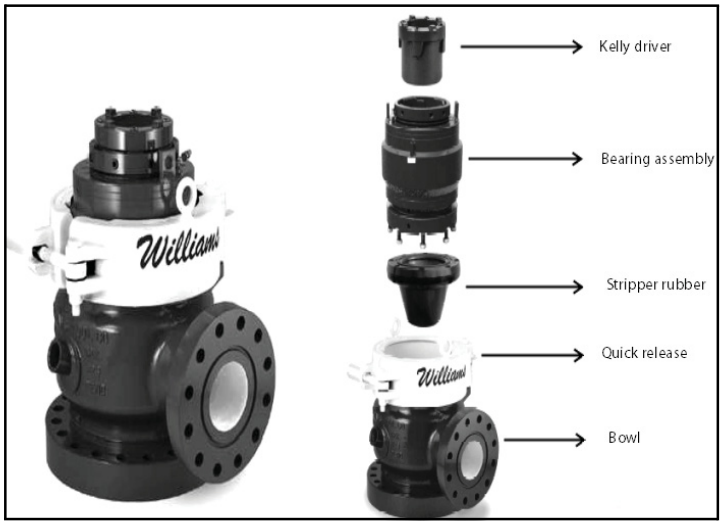
\includegraphics[scale=.7]{Figs/Fig2.PNG}
	\caption{Thiết bị kiểm soát áp suất\cite{rehm2013underbalanced}, $250 psi$}
	\end{figure}
\subsubsubsection{Bit float và String float} \\
	Trong chuỗi cần khoan cần có một thiết bị được gọi là Bit float được lắp đặt gần chòong khoan có chức năng giữ cho dòng trong giếng có thể chảy ngược về và bùn tại đáy giếng không bị kẹt lại. Bên cạnh Bit float còn có String float được lắp đặt ở phần đầu của chuỗi cần khoan có chức năng giữ cho áp suất trong toàn bộ chuỗi cần khoan không bị sụt giảm và tạo ra kết nối giữa các bộ phận.
\subsubsubsection{Fire float và Fire stop float} \\
	Ở một số quốc gia Fire float và Fire stop float được lắp đặt vào trong cần khoan ở phía trên cảu Bit float. Được sử dụng ở những vùng không chắc chắn về sự có mặt của Condensates trong giếng, thứ có thể trở thành nguyên nhân gây ra hiện tượng Downhole-fires. Trong trường hợp giếng có Downhole-fires, đai an toàn sẽ bị nóng chảy ra cho phép ống lót bịt kín cần khoan để có thể hạn chế được nguồn Oxy đi vào khu vực bị cháy. Quá trình này đồng thời làm tăng áp suất máy nén chính để mở máy nén nhánh.
	%\clearpage
	\begin{figure}[h]
	\centering
	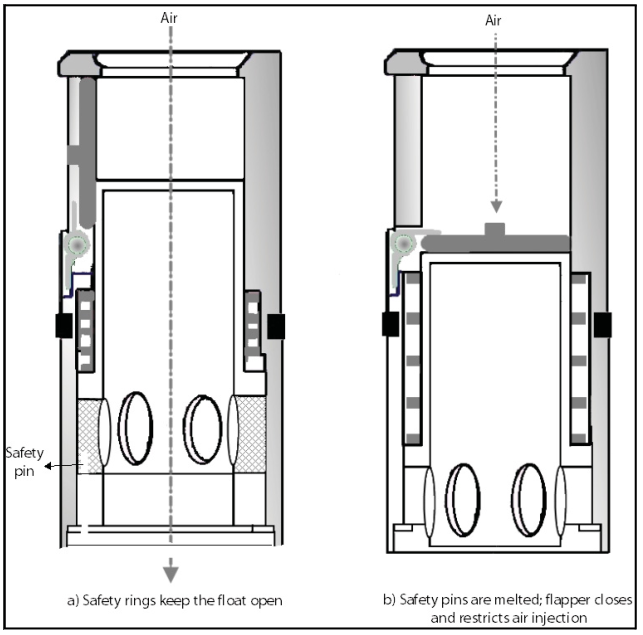
\includegraphics[scale=0.7]{Figs/Fig3.PNG}
	\caption{Fire float và Fire stop float\cite{rehm2013underbalanced}}
	\end{figure}
\subsubsubsection{Ống tháo cạn}\\
	Chiều dài ngắn nhất cần thiết để có thể sử dụng được ống tháo cạn vào khoảnh 200 đến 300 ft và diện tích mặt cắt ngang ít nhất phải bằng diện tích phần trên của khoảng không vành xuyến. Ống tháo cạn phải được đặt sao cho không bị đẩy lên bởi ảnh hưởng của khí hoặc dung dịch lỏng, đồng thời tránh trường hợp bị xoắn hoặc bị bẻ cong. Nếu áp suất trong ống tháo cạn thấp hoặc bằng áp suất khí quyển, việc đặt van đóng áp ở phía dưới cùng của ống là không cần thiết. Khi cần dừng việc tháo cạn nên đóng van trong đường áp suất cao hoặc ngay tại đầu giếng. Trong một số trường hợp, hai hoặc ba ống sẽ được đặt để đảm bảo sự thông gió của giàn.
\subsubsubsection{Bình tách, máy khử bụi, bộ giảm âm}\\
	Chức năng của những thiết bị này có thể được kết hợp chung vào một thiết bị duy nhất. Bụi có thể được kiểm soát bằng dòng nước trong ống tháo cạn và được làm lắng đọng như là bùn ở sàn rung. Những bình tách hay hay máy khử bụi cỡ lớn có thể hoạt động như một máy giảm âm để có thể triệt tiêu sóng âm trong ống tháo cạn.\\
	Hiện nay đã có nhiều giàn và các hệ thống thương mại được lắp đặt để có thể kiểm soát cổng xã của ống tháo cạn. Việc loại bỏ tích tụ tĩnh điện ở những hệ thống bình tách, máy khử bụi, máy giảm âm là cực kì quan trong, vì vậy những hệ thống này thường có một đầu được nối đất.\\
	Hầu hết trong kỹ thuật khoan bằng khí, lượng khí đều thoát ra theo ống tháo cạn, trừ khi lượng khi cần thiết để kiểm soát bui, sóng âm, hay tách dầu từ khí tự nhiên. Sử dụng bình tách kín sẽ an toàn hơn các loại bình tách khác, bìn kín sẽ tránh được hiện tượng va đậm giữa các phân tử bụi, khí và nước là nguyên nhân chính gây tĩnh điện trong các bình chứa.
\subsubsubsection{Hệ thống bơm khí}\\
	Khí được bơm vào ống góp phải khô và có nhiệt độ xấp xỉ nhiệt độ môi trường. Nếu sử dụng khí có nhiệt độ quá cao sẽ gây ảnh hưởng đến hệ thống ống quay dẻo, nếu khí ẩm sẽ làm cho khí khó được làm sạch. Vì vậy, hầu hết các máy nén khí hay máy tăng áp đều có một cấp làm lạnh và làm khô khí ở đầu ra.\\
	Trước khi được đưa vào sử dụng, các thiết bị như ống mềm dẫn khí từ máy nén hoặc máy tăng áp cần được thử áp suất ít nhất hai lần để có thể đảm bảo an toàn. Những vị trí như ống dẫn khí hoặc ống mềm từ máy nén áp suất tới ống góp của giàn khoan thường có nguy cơ lớn dẽ bị phá hủy do áp suất vượt quá tải. Khi trong ống dẫn chưa đầy khí nén, nếu ống bị vỡ tại các vị trí kết nối hay chia dòng, ống dẫn thường bị rung với một lực khá lớn. Ống dẫn cần được đặt cố định, đồng thời tại các vị trí kết nối cần có thêm đai an toàn.
\subsubsubsection{Bơm sương}\\
	Bơm sương là một thiết bị quan trọng trong hệ thống vận hành. Hai loại bơm thường dùng nhất là bơm sử dụng động cơ diesel và động cơ điện. Công suất của bơm thường nằm trong khoảng 0.5 gpm (2 l/m) tới 5 gpm (20 l/m), áp suất tạo ra lên tới 2,000 psi (14,000 kPa). Hệ thống động cơ bao gồm khớp ly hợp và bộ truyền động giúp cho bơm có thể làm việc ở áp suất cao hơn bình thường, ví dụ như áp suất cần thiết trong ống cuốn xoắn vào khoảng 5,000 psi.\\
	Hệ thống bơm sương cần có hai bể chứ nơi mà chất khử phụ gia và chất hóa học có thể được trộn với nhau để có thể tạo thành hỗn hợp bơm. Kích thước của bể tùy thuộc vào giếng, nhưng lượng dung dịch trong bể phải đảm bảo đủ đê hoạt động được ít nhất một giờ, vào khoảng 6 bbl hay 1 $M^3$. Phía bên trong bể thường có thước đo để định mức dung dịch trong bể.\\
	Khi khoan ở những vùng sa mạc hay những vùng có nguồn nước sạch khan hiếm, sương cần được làm sạch và xử lý độ cứng và các vi sinh vật trước khi đưa vào sử dụng. Nước cứng có thể để lại phần cặn bên trong cần khoan, trong một vài trường hợp có thể gây kẹt cần khoan.\\
	Nước nhiễm bẩn có thể gây ra một số vấn đề như tác động ăn mòn hóa học lên ống chống và cần khoan. Nước biển hoặc nước mặn có thể gây ra ăn mòn hóa học và làm giảm hiệu quả của các chất phụ gia khử sương.
\subsection{Phương pháp vận hành}
\subsubsection{Tuần hoàn dung dịch}
	Hầu hết khi sử dụng kỹ thuật khoan bằng khí khô vào một giếng nào đó, giếng đó sẽ được tháo tải. Cách dễ dàng nhất để tháo tải là thực hiện bơm khí từ phía dưới cùng của ống chống. Thực hiện quá trình này như sau: Sử dụng máy nén để tăng áp suất lên gần cực đại sau đó bơm đồng thời nước và khí cho đến khi áp suất bắt đầu giảm thì ngừng bơm. Thực hiện lại quá trình này cho đến khi giếng ngừng tải. Tỉ trọng trung bình của nước trong cần khoan tăng và áp suất máy nén giảm. Khi một phần của giếng bắt đầu ngưng tải, áp suất nén được giảm xuống.
\subsubsubsection{Làm khô giếng}\\
	Trong quá trình làm khô giếng, những phụ gia như chất tẩy khô, chất kiểm soát pH (KOH) hay chất ứng chế hơi nước được đưa vào giếng. Một số phương pháp khác có thể làm khô giếng là đưa khoảng một lít chất phụ gia hấp thụ nước, hơi nước xuống giếng trong khi đang tuần hoàn khí khô, hoặc đóng ram trong BOP và đưa áp suất lên khoảng 1000 psi, sau đó mở ram để nước trong giếng tự phun trào ra ngoài.\\
	Sau một vài giờ đưa khí khô vào giếng, giếng cần tiếp túc được khoan tiếp để có thể làm khô những phần ẩm còn lại trong giếng và ống chống. Ở giếng thân trần, việc làm khô giếng có rất nhiều khó khăn, hầu hết là bởi vì độ nhám của thành giếng.
\subsubsubsection{Vận hành}\\
	Trong giếng không còn dung dịch làm đệm cho sự dịch chuyển của cần khoan, đồng thời những vấn đề cso thể xảy ra bởi sự không thích hợp của tỉ trọng dung dịch tương đương. Bắt đầu khoan, đưa chòong khoan vào trong giếng, mở chốt trong của cần khoan. Bên cạnh những vấn đề nguy hiểm có thể xảy ra trên bề mặt, cần khoan có thể bị tuột nhanh ở trong giếng do không còn dung dịch đệm và có xu hướng bị xoắn lại khi xuống tới đáy. Vấn đề này thường khá khó để xử lý. Để hạn chế vấn đề này, khi khoan cần phải sử dụng khí ít nhất một lần ở khớp nối đáy để tránh trường hợp chòong khoan bị cắm sâu vào trong lớp bùn dưới đáy.\\
	Khí trong giếng thường có xu hướng tạo ra các rãnh dạng lỗ khóa và các lát đá mỏng trừ ở những giếng đã chống ống. Để tránh trường hợp cần khoan bị kẹt trong các rãnh dạng lỗ khóa, tốc độ thả cần khoan cần được giảm xuống ở một mức nhất định phù hợp với từng giếng.\\
	Các mối nối giữa các đoạn cần khoan thường bị hư hại khi thực hiện doa trong các đoạn giếng kích thướng nhỏ bởi vì lực xoắn thường lớn nhất ở vị trí các mối nối. Doa với chòong khoan ba chóp xoay cũng có thể làm xoắn thắt lại các bộ phận đỡ hoặc làm mòn chòong khoan ở những vị trí kích thước giếng nhỏ. Hiện tượng này xảy ra với mọi loại chòong khoan trong thành hệ cứng. Vì vậy, trước khi đưa chòong khoan vào giếng cần chắc chắn rằng kích thước giếng đủ rộng đối với chòong khoan.
\subsubsubsection{Kết nối}\\
	Ở những vị trí kết nói, giếng cần được tuần hoàn liên tục cho đến khi lượng mùn khoan giảm đến mức thấp nhất. Tại vị trí giếng có kích thước nhỏ, qua trình này thường không kéo dài quá mười phút. Nếu giếng có nhiều khe nứt, bề mặt thành giếng gồ ghề, thời gian làm sạch thường mất khoảng nửa giờ. Khi ngưng tuần hoàn, mùn khoan thường rơi ngược trở lại vào đáy giếng và tích tụ thành bùn ở các vị trí kết nối làm tăng thời gian làm sạch giếng ở những vị trí kết nối.\\
	Lực kéo tác động lên những vị trí kết nối thường phải được giảm đến thấp nhất. Không bao giờ được tác động lực kéo mạnh lên cần khoan nếu khoan ở vỉa khí ít thấm, quá trình cần được thực hiện từ từ. Nếu mùn khoan tích tụ nhiều xung quanh chòong khoan và cần nặng thường làm tắc thậm chí làm cho thành hệ càng bị nén chặt hơn. Nếu xuất hiện các vết nức dạng chìa khóa, quá trình nén chặt sẽ diễn ra nhanh hơn. Trong những giếng bị tắc, cần phải tuần hoàn khí liên tục và di chuyển cần khoan cho đến khi hết kẹt. Nếu không thành công, có thể áp dụng phương pháp đạp. 
\subsubsubsection{Làm sạch giếng}\\
	Nếu vận tốc khí ở khoảng không vành xuyến thấp, quá trình ``tắc nghẽn'' (choking) sẽ xảy ra ở những vị trí mùn khoan không được vận chuyển hoặc lơ lửng không thể thoát ra khỏi giếng. Bằng cách giảm áp suất máy nén cho đến khi vận tốc trong khoảng không vành xuyến tăng đến khi đủ khả năng có thể vận chuyển mùn khoan ra khỏi giếng. Đông thời khả năng vận chuyển mùn khoan còn phụ thuộc rất nhiều vào kích thước mùn khoan.\\
	Trong thực tế, kích thước mùn khoan phụ thuộc vào kích thước răng của chòong khoan, với chòong khoan có kích thước răng lớn, dài thường tạo ra mùn khoan kích thước lớn và cũng dễ gây ra hiện tượng ``Choking'' cho đến khi mùn khoan lại tiếp tục bị phá vỡ bởi dòng khí tuần hoàn. Mùn khoan có kích thước nhỏ giúp cho việc tăng tốc độ khoan và tăng khả năng làm sạch giếng của dung dịch khoan.
\subsubsubsection{Downhole fires}\\
	Sự cháy tức thời của hỗn hợp các Hydrocarbon nhẹ trong áp suất khí quyển có thể gây ra hiện tượng Downhole fires. Khi có mặt sự xuất hiện của Oxi trong hỗn hợp Hydrocarbon lỏng, khả năng gây cháy là rất lớn, nếu hỗn hợp đạt tới nhiệt độ cháy, Downhole firs có thể xảy ra. Downhole fires sẽ xảy ra tuần tự theo:
	\begin{itemize}
		\item Đầu tiên, có sự tích tụ của mùn khoan ở những vị trí có vận tốc dòng thấp, thường là ở phần cao nhất của cần nặng hoặc ở vị trí bị sói mòn do tuần hoàn dung dịch trong khoảng không vành xuyến.
		\item Hình thành đai bùn (mud rings). Khi có sự xuất hiện của dòng vào ở trong giếng, mùn khoan có thể sẽ gây bít kín xung quanh cần khoan hay thành giếng (ở những vùng có vận tốc dòng thấp).
		\item Hình thành các hang hốc kín xung quanh cần khoan, ở phía dưới vùng bị bít kín do mùn khoan.
	\end{itemize}
	Nếu khí tiếp tục được tuần hoàn trong khoảng không vành xuyến, làm tăng áp suất trong các hang hốc kín. Khi áp suất tăng, khí trong các hang hốc bị nén lại làm tăng nhiệt độ đến mức có thể gây cháy. Sự xuất hiện của hỗn hợp hydrocarbon lỏng chứa Oxi sẽ là tác nhân cuối cùng gây ra hiện tượng Downhole Fires. 
\subsubsection{Hệ thống tuần hoàn ngược}
	Trong hệ thống tuần hoàn ngược\cite{driscoll1986groundwater}, dung dịch khoan đi xuống giếng thông qua khoảng không vành xuyến và đi lên bên trong cần khoan đến của hút của máy bơm rồi được đưa vào bình chứa. Mùn khoan được đưa lên bên trong cần khoan thường có kích thước nhỏ hơn so với mù khoan trong khoảng không vàn xuyến. Phương pháp này thích hợp với những giếng có môi trường địa chất nhiệt độ cao và những giếng khoan khí. Sử dụng khí sẽ cho khả năng khoan được sâu hơn. Mực dung dịch trong khoảng không vành xuyến thường được giữ gần bằng với bề mặt.
	\clearpage
	\begin{figure}[h]
		\centering
		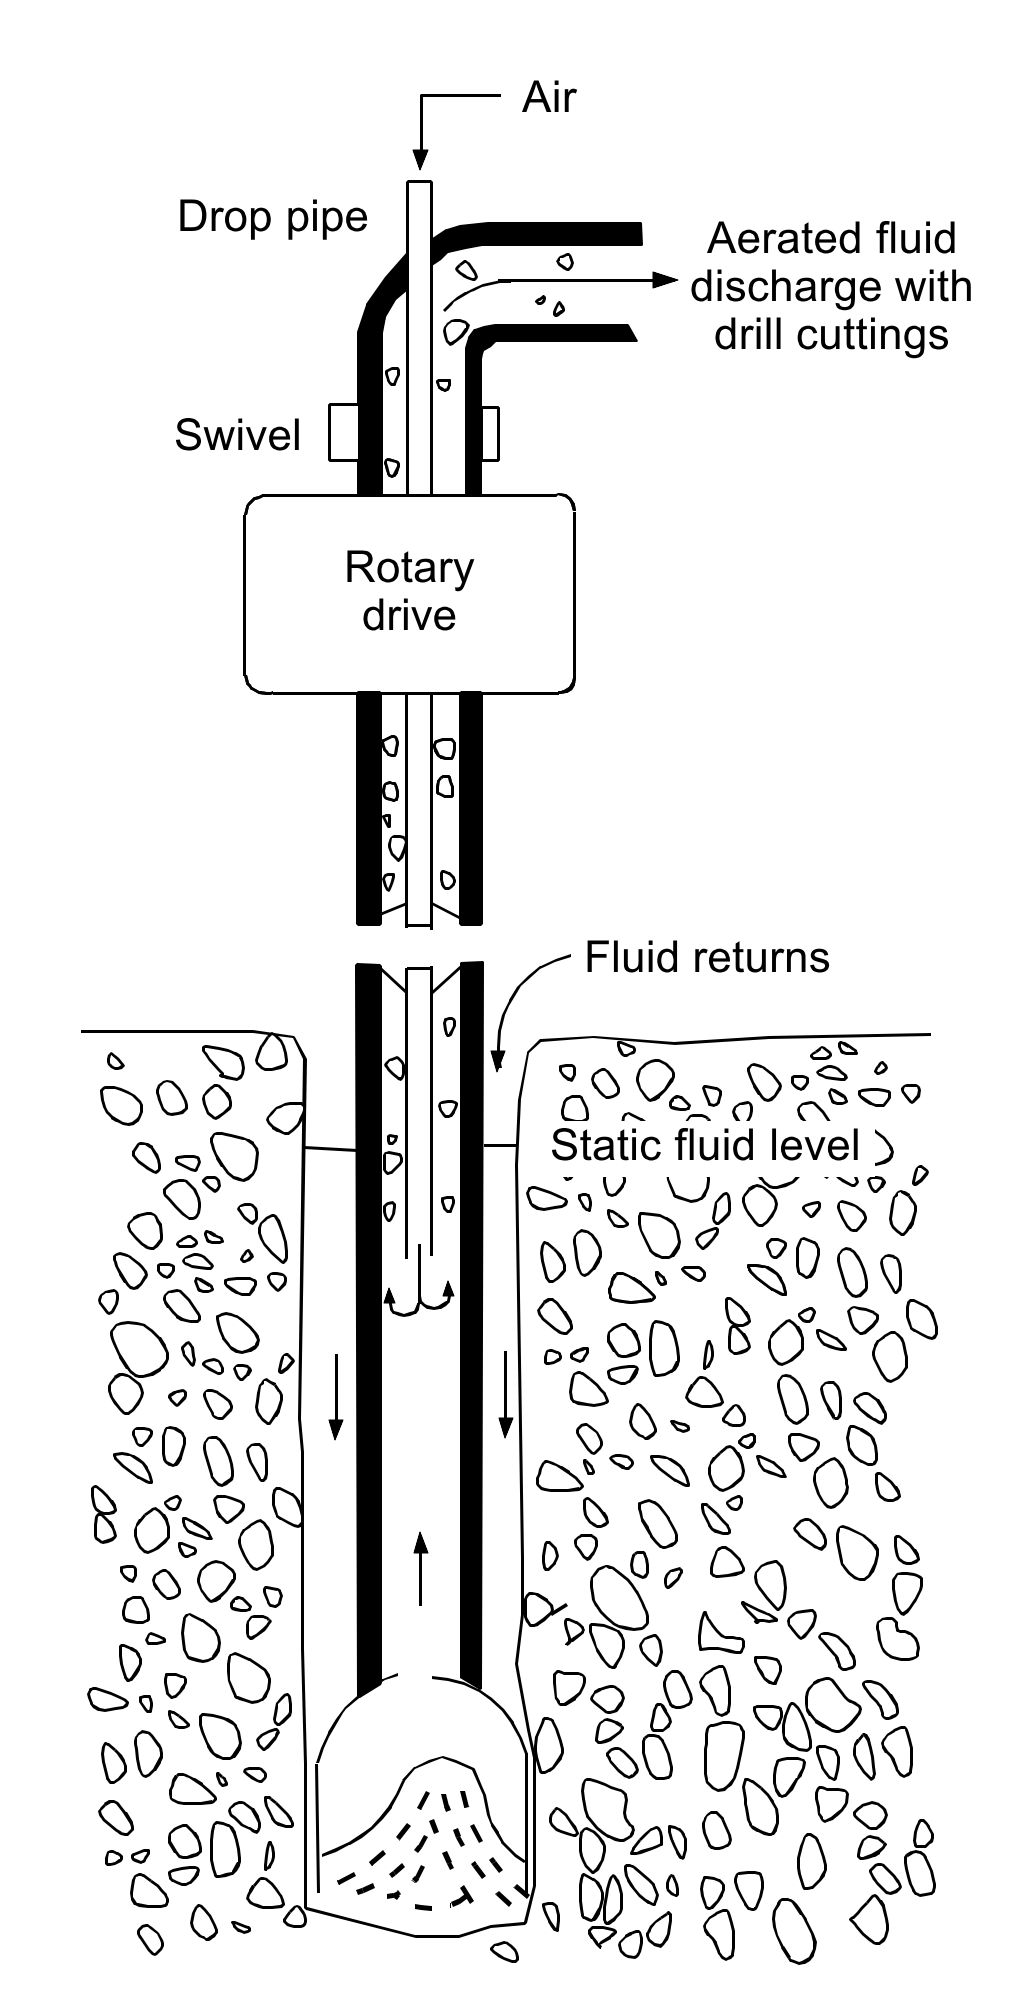
\includegraphics[scale=0.2]{Figs/Fig4.png}
		\caption{Hệ thống tuần hoàn ngược\cite{culver1998drilling}}
	\end{figure}
	Hệ thống tuần hoàn ngược mang lại nhiều lợi ích như:
	\begin{itemize}
		\item Giảm tốc độ của dung dịch trong khoảng không vành xuyến, vì vậy có thể hạn chế được vấn đề sói mòn thành giếng.
		\item Tăng tốc độ cảu dung dịch trong khoảng không vành xuyến, làm giảm thời gian vận chuyển mùn khoan, tăng chất lượng của mùn khoan được lấy mẫu.
		\item Giảm tác động của dung dịch khoan lên thành hệ.
	\end{itemize}
	Đồng thời cũng có một số giới hạn như:
	\begin{itemize}
		\item Mất mát dung dịch thường xảy ra nhiều ở những tầng có độ thấm cao. Tuy nhiên có thể hạn chế tối thiểu lượng dung dịch mất bằng cách thiết kế một chương trình khoan phù hợp.
		\item Khi mực dung dịch trong khoảng không vành xuyến ngang với bề mặt, nó ngăn cản sự xâm nhập của các nguồn địa nhiệt dưới áp suất vào trong giếng khoan gây khó khăn trong công tác đo đạt sự thay đổi của nhiệt độ hoặc hóa chất.
		\item Khi một số dung dịch địa nhiệt xâm nhập được vào giếng, nó làm thay đổi tính chất hóa học của dung dịch khoan, đồng thời có thể loại bỏ một số phụ gia đặc biệt trong dung dịch.
	\end{itemize}
	Một kĩ thuật thường dùng cho hệ thống tuần hoàn ngược là sử dụng cần khoan 6 in hoặc lớn hơn kết hợp với một máy bơm li tâm hoặc máy phun. Phương pháp này giới hạn cho giếng có đường kính từ 16 in trở lên, sử dụng tool joints có mặt bích đường kính 10 in trở lên để đảm bảo sự tuần hoàn của dung dịch trong giếng. Đối với những vỉa mỏng, không cố kết thường có xu hướng bị xói mòn, đôi lúc tạo ra những hang hốc nhỏ xung quanh mặt bích. Điều này gây khó khăn cho quá trình trám xi măng sau khi chống ống. Vì vậy, phương pháp này thường không được áp dụng cho những giếng có nguồn địa nhiệt không ổn định ngoại trừ một số giếng lớn có sử dụng bơm nhiệt.\\
	Một số kĩ thuật mới được sử dụng cho phép khoan những giếng có đường kính nhỏ sử dụng chòong ba chóp xoay, tăng khả năng khoan sâu và tốc độ khoan. Giảm thời gian tiếp cần hoặc kéo cần ra khỏi giếng.\\
\subsection{Kỹ thuật khoan bằng khí mù}
\subsubsection{Tổng quan}
	Khoan bằng khí mù\cite{rehm2013underbalanced} là một phần trong kỹ thuật khoan bằng khí. Khi muốn tăng khả năng vận chuyển mùn khoan và ngăn chặn hiện tượng "mud rings" ở thành hệ, người ta thường chuyển từ khoan bằng khí sang khoan bằng khí mù.\\
	Tỉ lệ nước khí phải tỉ lệ thuận với nhau để mang lại khả năng làm sạch giếng tốt nhất. Sự xuất hiện của nước trong khí làm tăng áp suất giếng. Khí nén cũng làm tăng áp suất giếng và giảm vận tốc dòng khí trong giếng.\\
	Với những giếng dễ bị ảnh hưởng trong khi vận hành, nước (hoặc chất lỏng) sẽ được bơm vào giếng tạo sương để có thể nâng cao khả năng vận chuyển mùn khoan của khí.
\subsubsection{Vận hành}
	Hầu hết để dừng vận hành hệ thống khoan bằng khí, người ta thường dùng hệ thống khí mù. Bơm một lượng nước vào hệ thống khí đủ để tạo ra sương, trong thực tế, khí mù được đưa vào vận hành chủ yếu để phục vụ hai mục đích chính:
	\begin{itemize}
		\item Phá hủy lớp mud cake được tạo thành từ nước vỉa và mùn khoan kích thước nhỏ trong quá trình khoan ở xung quanh thành hệ.
		\item Vận chuyển được mùn khoan kích thước lớn ra khỏi giếng.
	\end{itemize}

	%\clearpage
	\begin{figure}[h]
	\centering
	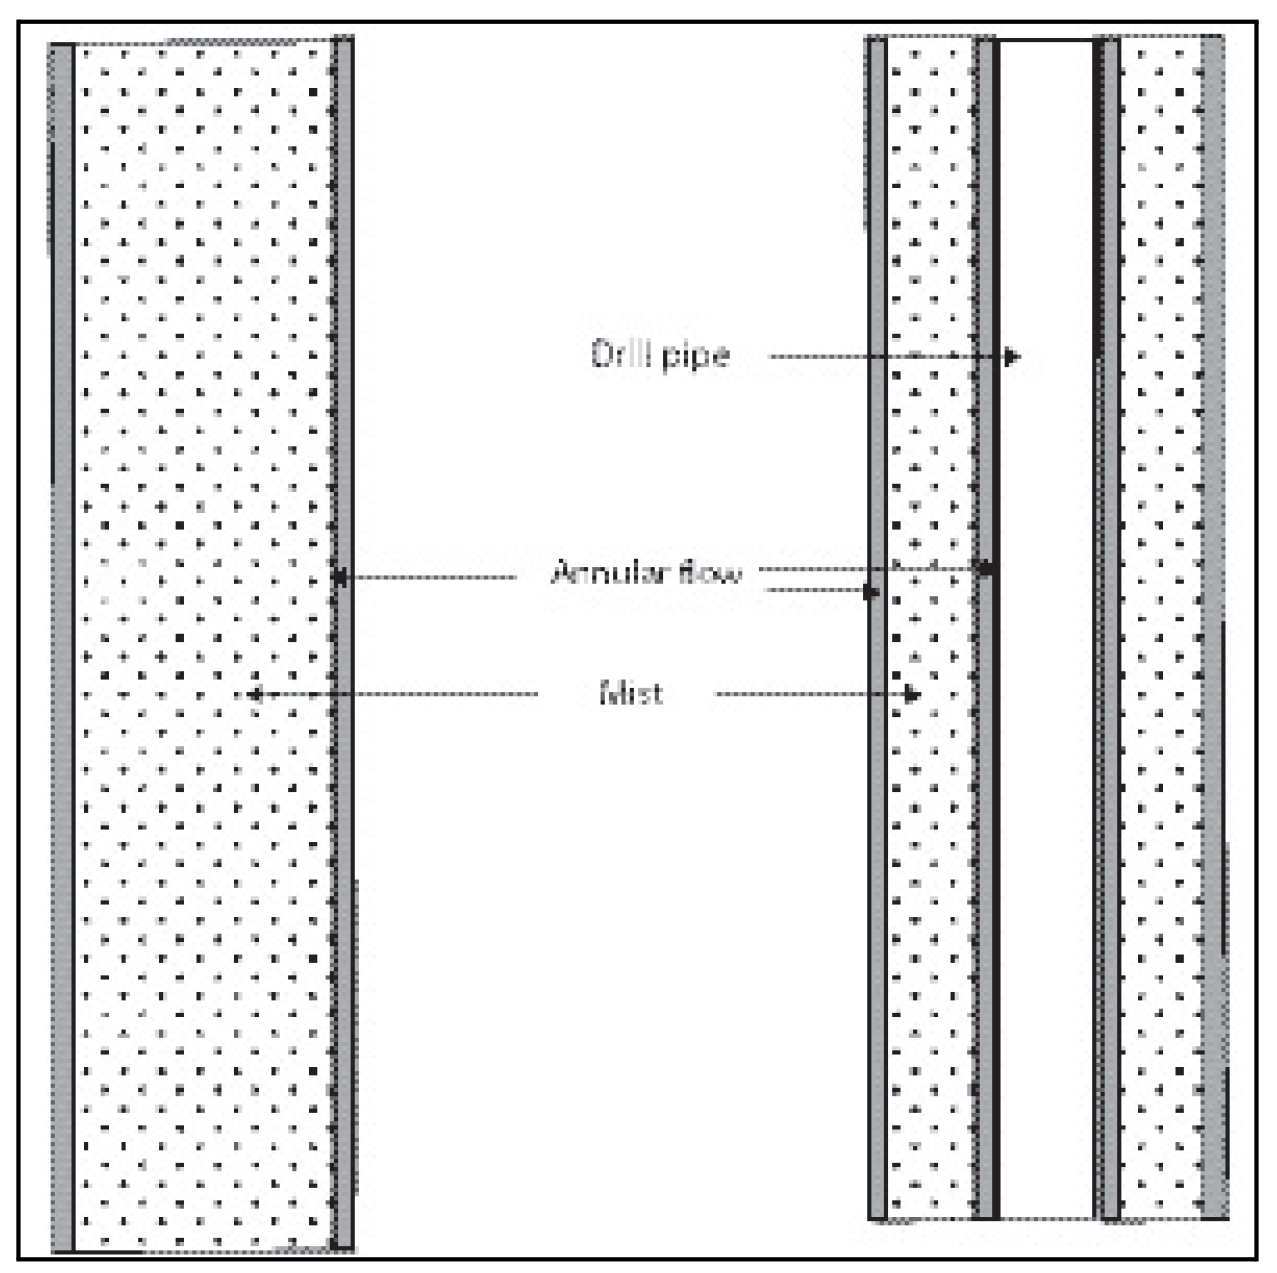
\includegraphics[scale=.3]{Figs/Fig6.png}
	\caption{Khí mù trong và ngoài cần khoan\cite{rehm2013underbalanced}}
	\end{figure}
	Hình 4 thể hiện quá trình tuần hoàn của khí mù trong khi khoan, pha khí có vận tốc lớn đẩy pha lỏng ra khỏi giếng. Pha khí di chuyển nhanh hơn pha lỏng và tạo ra lực cắt và dòng chảy rối tại bề mặt của lớp nước, loại bỏ các giọt nước nhỏ và mang chúng ra khỏi giếng.\\
	Trong khoan bằng khí mù, chất lượng của khí được giữ ở mức $95\%$ trong điều kiện đáy giếng. Đây là một khá không chính xác, bởi vì trong điều kiện đáy giếng lượng khí còn dư lại phụ thuộc vào kính thước mùn khoan. Tốc độ của pha khí và pha lỏng không bằng nhau, vì vậy việc tính toán thể tích khí và lỏng theo phương pháp thông thường sẽ có độ chính xác không cao. Việc tính toán thường rất phức tạp, sử dụng phương pháp lặp để có thể cân bằng được độ mỏng và lực cắt lên các lớp nước dưới đáy giếng.\\
	Khi ngừng việc bơm khí, các lớp nước bị rơi ngược trở lại xuống đáy giếng cùng với mùn khoan. Sau khi khí được bơm trở lại, sự chênh lệch vận tốc giữa pha khí và pha lỏng được tính toán bằng cách theo dõi khoàn thời gian dịch chuyển giữa thời gian dòng khí và dòng lỏng xuất hiện ở bề mặt.\\
	Hiện nay có nhiều kĩ thuật đưa chất phụ gia tạo bọt vào trong khoan khí mù. Bọt có khả năng làm sạch giếng tốt hơn tại vị trí chòong khoan và cần nặng. Có một vấn đề xảy ra khi thêm chất phụ gia tạo bọt vào dung dịch, đó là bọt có pha lỏng liên tục, khi pha khí trở thành pha liên tục và tạo thành dòng phun ở phần phía trên của giếng sẽ làm giảm khả năng vận chuyển mù khoan đồng thời dễ làm tắc cần khoan. Kĩ thuật sử dụng kết hợp khí mù và bọt là một kĩ thuật mang nhiều ưu điểm đồng thời cũng có nhiều hạn chế, vấn đề cần phải giải quyết.
\subsection{Kỹ thuật khoan bằng khí tự nhiên}
\subsubsection{Tổng quan}
	Khoan bằng khí tự nhiên\cite{rehm2013underbalanced} là một trong những kỹ thuật được dùng nhiều nhất cho đến năm 1970 khi giá thành của khí tự nhiên bắt đầu tăng mạnh, không còn phù hợp về mục tiêu kinh tế. Loại khí tự nhiên thường dùng trong kỹ thuật khoan này là metan ($CH_4$). Khí metan có những tính chất phù hợp với các yêu cầu cho một dung dịch khoan loại khí hoặc Gaseated hơn không khí hoặc những loại khí khác. Một số loại khí khác như etan ($C_2H_6$), propan ($C_3H_8$), butan ($C_4H_{10}$) hay một số hydrocarbon khác. Khí tự nhiên trong được dùng trong khoan thường có tỉ trọng 0.8.
\subsubsection{Ưu điểm}
\subsubsubsection{Chống ăn mòn}\\
	Một trong những ưu điểm lớn nhất của việc sử dụng khí tự nhiên là không gây ăn mòn hóa học lên thiết bị lòng giếng, khí tự nhiên không chứa Oxy, vì vậy sẽ không gây ra những vấn đề ăn mòn hóa học. Ăn mòn hóa học trong khi khoan luôn là một vấn đề gây tốn nhiều chi phí, sử dụng khí tự nhiên trong khi khoan sẽ giúp xử lý vấn đề này.
\subsubsubsection{Down-Hole Fires}\\
	Vì không chứa Oxy nên khi sử dụng khí tự nhiên có thể tránh được hiện tượng Downhole Fires.
	Khí ở xung quanh miệng giếng và ở dưới sàn khoan có thể gây ra nhiều nguy hiểm, vì vậy cần được thông gió tốt để có thể thoát khí khi lượng khí tích tụ quá nhiều. Khí tự nhiên nhẹ hơn không khí nên thường có xu hướng tập trung nhiều ở đòn quay hoặc những không gian kín tương tự. Hiện tượng này thường xảy ra ở những nơi có khí hậu lạnh, cấu trúc dưới giàn thường dễ bị đóng lại do nhiệt độ.
\subsubsubsection{Tiện lợi}\\
	Khi áp suất nguồn khí tự nhiên có thể được gia tăng bằng cách sử dụng đường ống dẫn khí, điều này mang lại nhiều lợi ích cho nhà thầu, nguồn khí thuận tiện hơn, giá thành rẻ hơn so với việc sử dụng máy nén khí.
\subsection{Kỹ thuật khoan bằng bọt}
\subsubsection{Tổng quan}
	Khoan bằng bọt là phương pháp sử dụng hệ thống dung dịch khoan bằng bọt, với những ưu điểm như giảm độ nhớt của dầu, tăng khả năng làm sạch giếng. Dung dịch đồng thời giúp giảm bớt mất mát dung dịch vì sự giảm nở của các bọt khí khi chúng được tuần hoàn đến vùng có áp suất thấp. Dung dịch bọt thường có những tính chất sau đây:
	\begin{itemize}
		\item Tăng cường khả năng đưa dầu lên mà không phụ thuộc vào tốc độ.
		\item Khả năng ổn định trong dòng có tỉ trọng thấp.
		\item Ngăn chặn, giảm thiểu mất dung dịch.
		\item Bảo vệ thiết bị khỏi ăn mòn hóa học.
	\end{itemize}
	Bọt là một loại dung dịch nhũ tương khi bơm khí vào trong nước (đôi khi là dầu), với nước ở trạng thái liên tục. Những hoạt chất bao quanh mỗi bọt khí giữ cho nó không kết hợp với các bọt khí xung quanh.
\subsubsection{Khả năng làm sạch giếng}
	Dung dịch bọt có khả năng vận chuyển mùn khoan tốt. Khả năng làm sạch tốt nhất nếu lượng bọt trong dung dịch từ $50\%$ đến $90\%$\cite{rehm2013underbalanced}. Trên $90\%$, dung dịch bọt sẽ chuyển sang pha khí liên tục và mất đi khả năng vận chuyển mùn khoan, dưới $50\%$ sẽ làm giảm khả năng vận chuyển của dung dịch. Trong giếng khoan ngang lượng bọt nằm trong khoảng $30$ – $40\%$ là tốt nhất.
\subsubsection{Hệ thống thiết bị}
%\clearpage
	\begin{figure}[h]
	\centering
	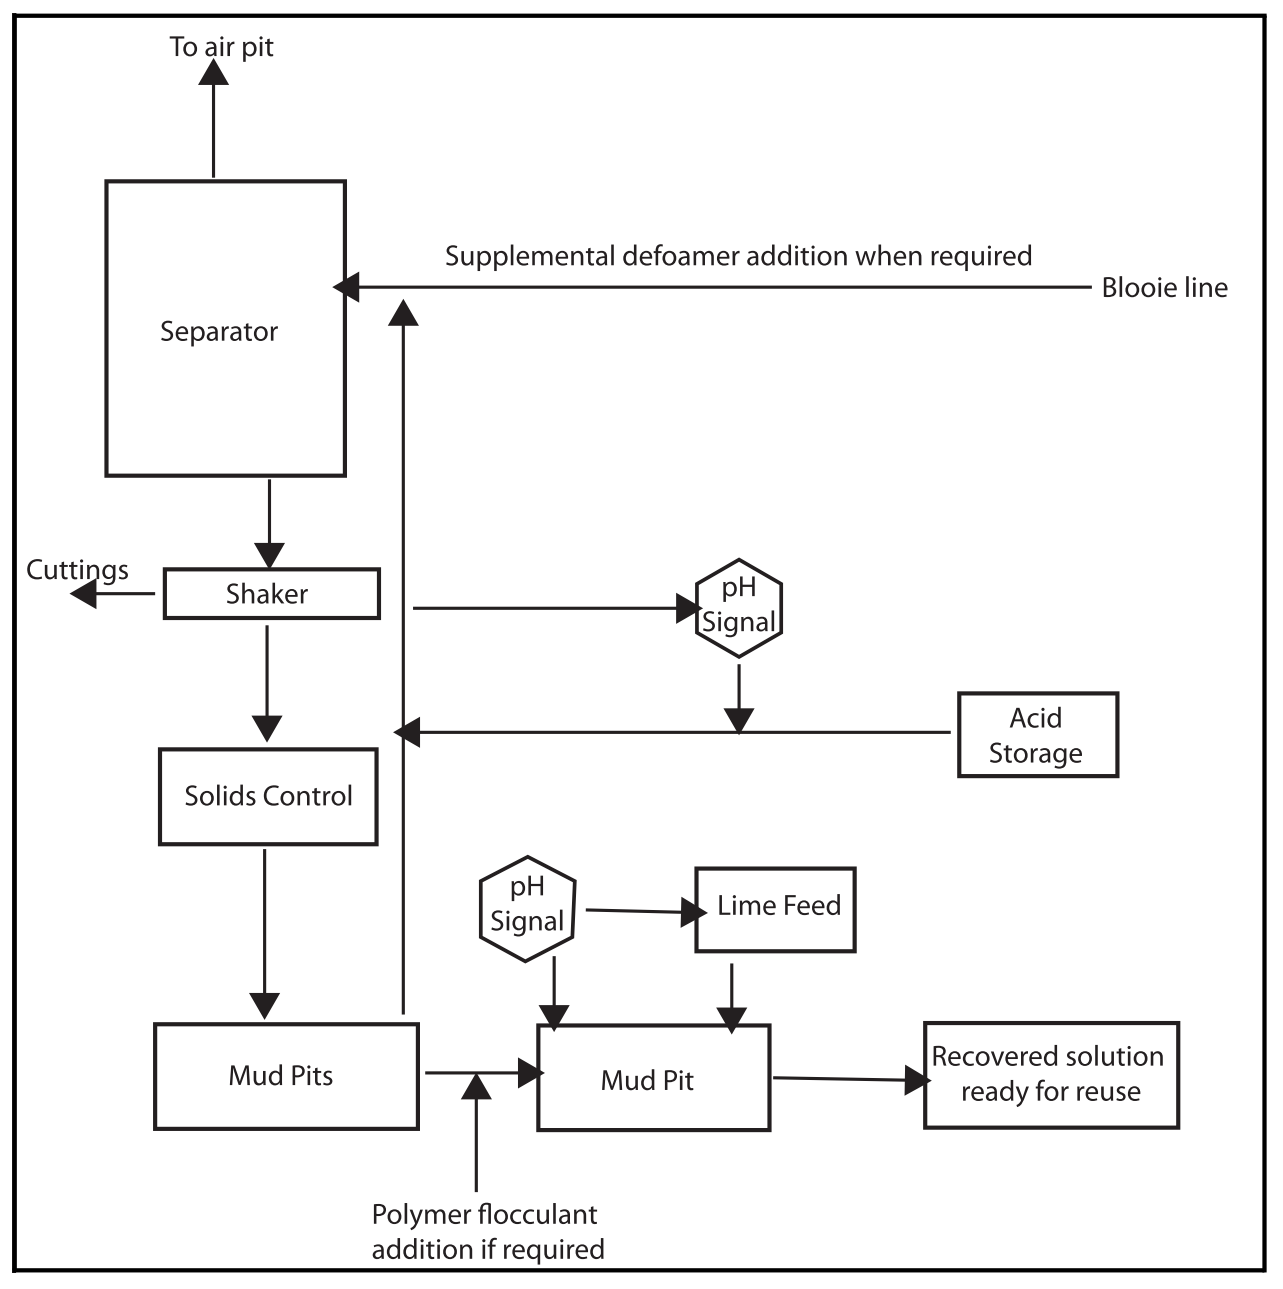
\includegraphics[scale=0.4]{Figs/Fig5.png}
	\caption{Hệ thống thiết bị khoan bằng dung dịch bọt\cite{rehm2013underbalanced}}
	\end{figure}
	\newpage
\subsubsection{Thành phần dung dịch}
	\subsubsubsection{Dung dịch bọt gốc nước}\\
	\textbf{Nước nguyên chất}\\
	Hầu hết dung dịch bọt đều sử dụng nước là pha liên tục và thường là nước thương mại (nước có thể uống). Mọi sự thay đổi về thành phần đều làm thay đổi giá thành của dung dịch (thường là tăng) và mức độ ổn định của bọt (thường là giảm). Nước nhiễm bẩn cần được xử lí trước khi thêm các phụ gia tạo bọt, đồng thời loại bỏ được các thành phần gây ăn mòn hóa học như các ion âm hay vi sinh vật.\\
	\textbf{Nước biển}\\
	Được sử dụng ở những khu vực khô hạn khi mà nguồn nước nguyên chất trở nên khan hiếm, nước biển hay nước mặn được sử dụng để làm pha liên tục cho dung dịch bọt. Khi sử dụng nước biển cần sử dụng một số phụ gia đặc biệt để sử lý độ “cường” của nước ($Na^+$, $Ca^{2+}$) thường là soda dư ($NaCO_3$). Tuy nhiên cần phải cẩn thận khi sử dụng soda dư, vì khi sử dụng sẽ dễ dàng hình thành gốc bicarbonate ($HCO_3^-$) gây ra ăn mòn hóa học. Những chất phụ gia đặc biệt này thường khá tốn kém, cần được xem xét trước khi sử dụng.
	\subsubsubsection{Dung dịch bọt gốc dầu}\\
	Khi dung dịch gốc nước trở nên nhạy cảm với vỉa (Nhiệt độ cao hay chứa nhiều chất nhiễm bẫn), dung dịch bọt gốc dầu, OleoFoam HT, được sử dụng để quá trình khoan trở nên thuận lợi ở những vỉa nhạy cảm với nước. Dung dịch gốc dầu có khả năng ổn định ở nhiệt độ lên tới $450^oF$, vì vậy thường xuyên được áp dụng ở môi trường có nhiệt độ khắc nhiệ
	Dung dịch bọt gốc dầu (OBFDF, Oil-based foam drilling fluid) thường được sử dụng cho những môi trường đặc biệt, vì vậy cần được thiết ké theo một tiêu chuẩn nhất định. Một số tiêu chuẩn được thiết lập để vận hành trong những điều kiện đặc biệt như tiêu chuẩn của Weatherford:
	\begin{itemize}
		\item Dung dịch gốc cần tương thích với các phụ gia phổ biến như các chất ức chế ăn mòn, cặn.
		\item Mức độ tạo bọt phải lớn hơn 130mL, vòng đời của bọt phải lớn hơn ba phút. Mức độ tạo bọt là thể tích bọt được tạo ra bằng cách trọn chất tạo bọt vào 100mL dung dịch gốc. Vòng đời của bọt được tinha bằng thời gian 50mL dung dịch bọt bị phá vỡ hoàn toàn.
		\item Dung dịch phải tương thích với các thiết bị lòng giếng.
		\item Hệ thống vận hành phải đủ điều kiện để có thể vận hành với mọi loại dung dịch gốc dầu trong bản thiết kế dung dịch khoan.
		\item Dung dịch phải có khả năng tái sử dụng, dung dịch tái sử dụng phải hoạt động tốt.
		\item Dung dịch phải tương thích với quá trình lọc dầu ở các nhà máy lọc dầu để tạo ra những sản phẩm có giá trị thương mại.
	\end{itemize}
	\textbf{Phụ gia tạo bọt dầu:}\\
	Khi độ ổn định của bọt quá thấp làm cho vòng đời của bọt bị rút ngắn, phụ gia dầu tạo bọt được đưa vào dung dịch. Khi sử dụng phụ gia này pha liên tục thường là dầu thô, diesel, dầu khoáng hay các hợp chất của olefin hoặc este. Dung dịch bọt loại này thường ổn định ở nhiệt độ cao hay những vị trí phức tạp khó giải quyết bằng cách vận hành loại dung dịch thông thường.\\
	Các chất phụ gia kích thích hoạt động bề mặt thường dùng là silicon oligomer, có khả năng thay đổi linh hoạt để tương thích với điều kiện hoặc thiết kế thể tích, vòng đời mong muốn kể cả những vị trí có mật độ bọt thấp.\\
	\textbf{Phụ gia khử bọt:}\\
	Thường sử dụng gốc silicone, khi sử dụng chất khử bọt quy trình tuần hoàn thường là “tạo bọt – khử bọt – tái tạo bọt” và vẫn có thể giữ được tính chất mong muốn ban đầu của dung dịch bọt. Thực tế, hầu hết các chất khử bọt tốt như alcohols, ete, hợp chất hydrocarbon hoặc một số hợp chất khác đều không tương thích với chất tạo bọt gốc silicone hay chất làm tăng độ nhớt.\\
	\textbf{Phụ gia tăng độ nhớt:}\\
	Thường sử dụng một số polime hòa tan trong dầu trên thị trường nhưng hầu hết đều không phù hợp với các công thức tạo dung dịch khoan gốc bọt. Hiện nay, Styrene-Isoprene thường được sử dụng để thiết kế những tính chất mong muốn cho dung dịch bọt. Những hợp chất đồng trùng hợp thường được sử dụng cho môi trường khoan có nhiệt độ cao, tăng độ nhớt của pha liên tục (pha lỏng), cho phép điều chỉnh tính chất bọt tùy thuộc vào điều kiện khoan như vận chuyển mùn khoan hay kiểm soát áp suất đáy giếng.
\subsubsection{Hạn chế}
	Giá thành, một trong những yếu tố chủ yếu làm tăng giá thành của dung dịch bọt là các chất phụ gia tạo bọt và các hợp chất hóa học có chức năng ổn định và kiểm soát ăn mòn. Giá thành của dung dịch bọt thay đổi theo kích thước giếng, tính chất hóa học cần thiết cho những giếng có nhiệt độ trên $200^oF$ hoặc giếng có điều kiện khai thác khắc nhiệt. Chất tạo bọt hóa học khá phổ biến đối với những dự án lớn, vì vậy chi phí sẽ giảm tương đối đáng kể nếu được mua theo số lượng lớn.\\
	Đối với những giếng có nhiệt độ khắc nhiệt, trên $200^oF$, dung dịch bọt có xu hướng di chuyển như dung dịch khí, làm mất đi khả năng ổn định, kiểm soát áp suất, làm sạch mùn khoan trong giếng.\\
	Trong trạng thái nhũ tương dung dịch bọt khá ổn định, với lớp màng có khả năng chống phá vỡ trong điều kiện vỉa muối nóng, vỉa nước chứa acid. Tuy nhiên, dung dịch bọt có xu hướng bị phân tách trong quá trình tuần hoàn, lúc đó phần dung dịch bị nhiễm bẩn sẽ nhanh chóng bị phá hủy bởi vì dầu nhẹ, khoáng vật nhiệt độ cao hay nước chứa acid đều làm những tác nhân khử bọt tốt. Một số phương pháp giải quyết vấn đề này như:
	\begin{itemize}
		\item Giảm dòng vào bằng cách tăng áp suất bề mặt.
		\item Tăng áp suất đáy giếng bằng cách tăng thể tích lượng nước trong dung  dịch bọt để làm tăng tỉ trọng dung dịch bọt.
		\item Thêm chất phụ gia làm tăng độ ổn định cho dung dịch bọt.
		\item Không tái sử dụng dung dịch bọt, thay vào đo, sử dụng hệ thống tuần hoàn dung dịch đơn.
	\end{itemize}
\subsection{Kỹ thuật khoan bằng bọt sánh}
	Khoan bằng bọt sánh\cite{rehm2013underbalanced} là một kỹ thuật mở rộng trong kỹ thuật khoan bằng bọt. Kỹ thuật này được sử dụng để khoan vào những thành hệ có độ cố kết thấp, cần dung dịch khoan có tỉ trọng thấp nhưng cần thêm vào các phụ gia có chức năng ổn định thành hệ. Lớp màng của bọt sánh có độ bền cao hơn so với bọt nên có khả năng vận chuyển mùn khoan có kích thước lớn hơn. Khi sử dụng dung dịch bọt sánh, tốc độ dung dịch ở khoảng không vành xuyến tăng từ 100 đến 200 ft/min, vì vậy không cần thiết phải sử dụng hệ thống nhiều máy nén như các loại khí khác.(Có thể thay đổi tốc độ dung dịch tùy thuộc vào lượng chất lỏng chảy vào giếng từ thành hệ.)\\
	Dung dịch bọt sánh được sử dụng để vận chuyển mùn khoan trong những giếng khoan đường kính lớn, trong những thành hệ có độ cố kết yếu. Thành phần của các chất phụ gia trong dung dịch bao gồm bentonit là 10 - 15 lb/bbl, với gôm polisacarit là 0.2 - 0.5 lb/bbl, với soda khan là 1 lb/bbl và một số chất phụ gia tạo bọt khác được đưa vào bằng khoảng 1\% thể tích. Có thể sử dụng bentonit peptit hóa cho bentonit và một số loại pomymer hữu cơ khác cho gôm polisacarit. Dòng dung dịch tuần hoàn ngược trở lại thường có độ nhớt cao hơn so với dung dịch ban đầu do sự có mặt của lớp bùn trong giếng, vì vậy dung dịch bọt sánh phải được bơm vào giếng với tốc độ cao để có thể tạo ra dòng tuần hoàn ngược. \\
	Hệ thống kiểm soát dung dịch bọt sánh cần có một máy bơm thể tích nhỏ để bơm vật liệu tạo bọt vào dòng khí. Ngoài ra còn có thể sử dụng máy tạo bọt để đưa bọt thẳng vào trong đường ống. Thành phần của dung dịch được lựa chọn sao cho có thể cung cấp khả năng ổn định cho dung dịch trong những môi trường khác nhiệt như nước vỉa chứa muối hay trong dầu. Trong những môi trường này bentonit thường không được sử dụng.\\
	Một yếu tố ảnh hưởng đến mức độ hoàn thiện của dung dịch bọt sánh là khả năng duy trì cột dung dịch bọt sánh liên tục từ ống dân bùn khoan đến ống tháo cạn. Áp suất bề mặt, momen xoắn của chuỗi cần khoan, mức độ liên tục và hình dạng bọt của dung dịch tại ống tháo cạn là những yếu tố cần phải xem xét khi thay đổi thành phần và tốc độ bơm dung dịch. Tốc độ khoan và kích thước mùn khoan cũng là những thông số quan trọng cần được xem xét.
\subsection{Kỹ thuật Snub drilling}
\subsubsection{Tổng quan}
	Snub drilling\cite{rehm2013underbalanced} là phương pháp kiểm soát sự chuyển động của cần khoan khi ra vào giếng khoan trong khi vẫn tiếp tục kiểm soát giếng. Không giống với những phương pháp khoan và hoàn thiện giếng truyền thống, kĩ thuật này yêu cầu phải sử dụng dụng dịch giảm tỉ trọng, điều này thường làm tăng giá thành giếng khoan, gây hư hại thành hệ.\\
	Hệ thống snubbing có thể trợ giúp quá trình vận hành giàn khoan khi xuata hiện áp suất bề mặt. Bình thường snubbing thường được thực hiện trong khi giếng đang trong trạng thái khoan dưới cân bằng. VÌ vậy, các phương pháp và thiết bị kiểm soát áp suất (thường là BOP) cần được sử dụng để giữ dụng dịch nằm trong tầm kiểm soát.
\subsubsection{Thiết bị}
	\subsubsubsection{Hệ thống thủy lực}\\
	Hệ thống thủy lực được đưa vào sử dụng vì có những ưu điểm như hệ thống điều khiển chuẩn xác bằng tay, hệ thống thủy lực thường nhanh và có phản hồi chuẩn xác trong thời gian tương ứng. Mọi thay đổi về áp suất bằng cách điều khiển van đều được phản hồi gần như ngay lập tức ở mọi vị trí trong hệ thống. Hệ thống thủy lực dùng để điều khiển chuyển động của cần khoan, tubing, ống chống thông qua búa thủy lực, đối áp vành xuyến. Van an toàn dùng để ngăn cản áp suất quá tải. Đặc tính an toàn này có thể loại bỏ những sai sót trong vận hành do con người.
	\subsubsubsection{Hệ thống Snubbing}\\
	Hệ thống Snubbing có thể chia thành bốn phần cơ bản như sau:
	\begin{itemize}
		\item Hệ thống thiết bị cơ bản
		\item Cột ống và thành phần cột ống
		\item Hệ thống thiết bị kiểm soát giếng
		\item Thiết bị phụ.
	\end{itemize}
	\begin{enumerate}
		\item Hệ thống Snubbing cơ bản\\
		Hệ thống thiết bị cơ bản thường là những hệ thống thủy lực hay cơ khí được dùng để tạo lực đẩy, kéo, xoắn lên chuỗi cần khoan. Ba loại hệ thống đẩy thường dùng là hệ thống kích thủy lực, hệ thống thủy lực hành trình dài, hệ thống nâng cơ khí ``Rig assist''.\\
		``Rig assist'' và hệ thống kích được sử dụng rất phổ biến trong hệ thống thiết bị Snubbing vì khả năng xử lý được nhiều vấn đề xảy ra với giếng. Kích có thể vận hành được cả trên giàn truyền thống và giàn phi truyền thống.\\
		Những ưu điểm của ``Rig assist'' so với các loại khác như là:
		\begin{itemize}
			\item Hiệu suất cao
			\item Khả năng chịu xoắn tốt
			\item Thiết kế gọn nhẹ
			\item Thích hợp với nhiều loại ống từ $\dfrac{3}{4}$ đến $13\dfrac{3}{8}$ in.
			\item Lực tác động chủ yếu lên đầu giếng, giúp giảm bớt phá hủy thành hệ, mang lại nhiều lợi ích trong khi khoan
			\item Có thể thay đổi trọng lượng của thiết bị để có thể phù hợp với quá trình lắp đặt.
		\end{itemize}
		Hạn chế của ``Rig assist'':
		\begin{itemize}
			\item Thời gian kéo ống và tiếp ống lâu hơn
			\item Quá trình lắp đặt khó khăn
			\item Sử dụng chuỗi cần khoan đơn.
		\end{itemize}
		\clearpage
		\begin{figure}[h]
			\centering
			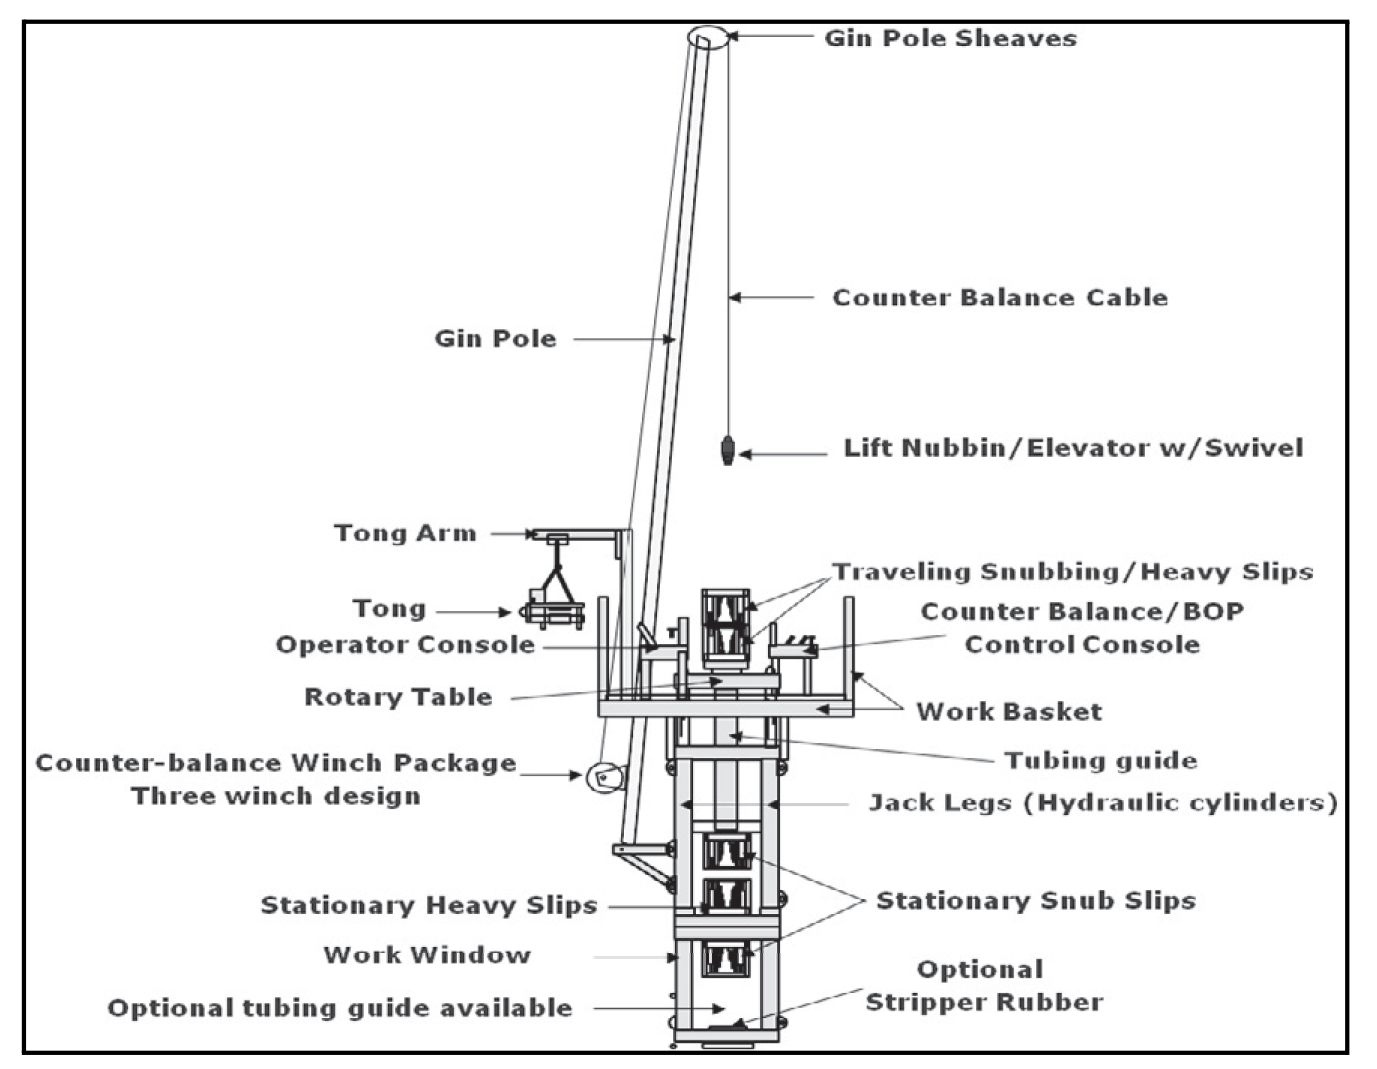
\includegraphics[scale=.4]{Figs/Fig7.png}
			\caption{Hệ thống Snubbing\cite{rehm2013underbalanced}}
		\end{figure}
		\begin{figure}[h]
			\centering
			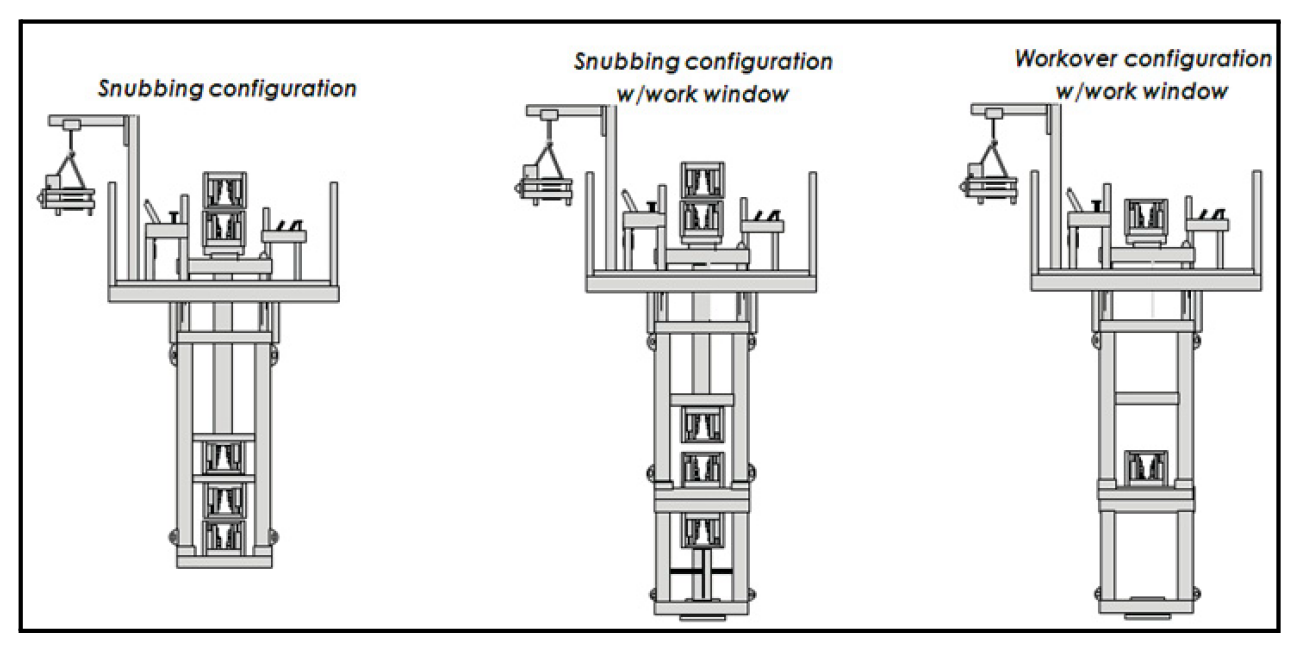
\includegraphics[scale=0.4]{Figs/Fig8.png}
			\caption{Hệ thống Snubbing cơ bản\cite{rehm2013underbalanced}}
		\end{figure}
		\item Thành phần chuỗi cần khoan
		\begin{itemize}
			\item Van đối áp
			\item Stabbing van
			\item BOP
			\item Khớp nối vòng tuần hoàn
			\item Ống tuần hoàn
			\item Ống nối
			\item Bộ khoan cụ và thành phần bộ khoan cụ.
		\end{itemize}
		\item Hệ thống kiểm soát giếng \\
		Hệ thống kiểm soát sơ cấp:\\
		Gồm ba thành phần đĩa cao su, đầu bịt an toàn dạng vòng, ram.\\
		Đĩa cao su được dùng để có lập không gian giữa các bộ phận, loại bỏ hiện tượng ``Ram to ram stripping'' trong những giếng áp suất thấp, rút ngắn thời gian bảo trì trong khi khoan. Có nhiều loại đĩa cao su và thường được lắp đặt ở giá đỡ snubbing.\\
		Đầu bịt an toàn dạng vòng thường được dùng để kiểm soát dung dịch khoan. Ngoài ra còn dùng cho mục đích tháo lắp, nhưng thường chỉ được sủ dụng trong giai đoạn kiểm soát giếng thứ cấp.\\
		Ram và những bộ phận liên quan được sử dụng thường xuyên trong hệ thống snubbing, cho phép kiểm soát di chuyển của ống với áp suất bề mặt. Những bộ phận cơ bản của ram:
		\begin{itemize}
			\item Stripper pipe ram
			\item Hệ thống cuộn cân bằng
			\item Hệ thống xả áp
			\item Van cản dòng.
		\end{itemize}
		Hệ thống kiểm soát thứ cấp: \\
		Mục đích của kiểm soát thứ cấp là tiếp tục duy trì kiểm soát giếng trong trường hợp xảy ra vấn đề không mong muốn hoặc trong thời gian bảo trì hệ thống kiểm soát thứ cấp.\\
		Những bộ phận và thành phân của BOP trong bộ kiểm soát thứ cấp thường tùy thuộc vào nhà sản xuất và mục đích sử dụng, bao gồm những bộ phận cơ bản sau:
			\begin{itemize}
				\item Hai ống ram
				\item Một ram đóng, một ram cắt
				\item Đường tiết lưu, đường bơm dung dịch dập giếng.
			\end{itemize}
		Hệ thống kiểm soát tam cấp:\\
		Mục tiêu của kiểm soát tam cấp là tiếp tục kiểm soát giếng trong trường hợp khẩn cấp hoặc trong thời gian bảo trì hệ thống kiểm soát sơ cấp và thứ cấp. Hệ thống kiểm soát tam cấp bao gồm ram cắt đơn với hệ thống kiểm soát độc lập.\\
		Hệ thống kiểm soát chính được đặt ở work basket, tránh xa miệng giếng khoan để giữ an toàn khỏi rò rỉ khí dễ gây cháy nổ.
		\item Hệ thống thiết bị phụ\\
		Hệ thống nâng giữ cần khoan và work basket: Được thiết kế nhằm mục đích di chuyển ống ra vào giếng đồng thời lắp đặt để kết nối chuỗi cần khoan ra vào giếng. Hệ thống nâng giữ cần khoan được vận hành trong quá trình vận hành hệ thống HWO/Snubbing:
			\begin{itemize}
				\item Nhận và tiếp cần từ work basket
				\item Tạo lực xoắn lên cần bằng cả hai phương pháp tay và thủy lực
				\item Không cần tháo bỏ các bộ phận kết nối, vòng tuần hoàn, ống tuần hoàn trong quá trình bảo trì.
			\end{itemize}
		Work basket được đảm bảo an toàn bằng cách sử dụng lối vào là một cầu thang, ngoài ra lối thoát hiểm khẩn cấp được lắp đặt. Lối thoát hiểm khẩn cấp được lắp đặt bằng một trong những cách sau:
			\begin{itemize}
				\item Dây cáp geromino
				\item Cánh cháy
				\item Catwalk 
				\item Cầu thang thoát hiểm.
			\end{itemize}
	\end{enumerate}
\subsection{Kỹ thuật khoan bằng khí Nitơ}
\subsubsection{Nitơ màng}
	Nitơ màng\cite{rehm2013underbalanced} được tọa ra bằng cách bơm khí đi xuyên qua một hệ thống màng gồm nhiều hợp chất có khả năng giữ lại phân tử nitơ nhưng cho phép các phân tử khác như oxi, carbon dioxide và phân tử hơi nước đi qua. Một phần phân tử khí oxi bị giữ lại trong màng cùng khí nitơ, lượng khí oxi này tùy thuộc vào áp suất qua màng, áp suất càng lớn thì lượng khí bị giữ lại càng ít. Màng nitơ sử dụng khi muốn hỗn hợp khí có từ 4 đến 5\% khí oxi cộng với các khí khác. 
	%\clearpage
	\begin{figure}[h]
	\centering
	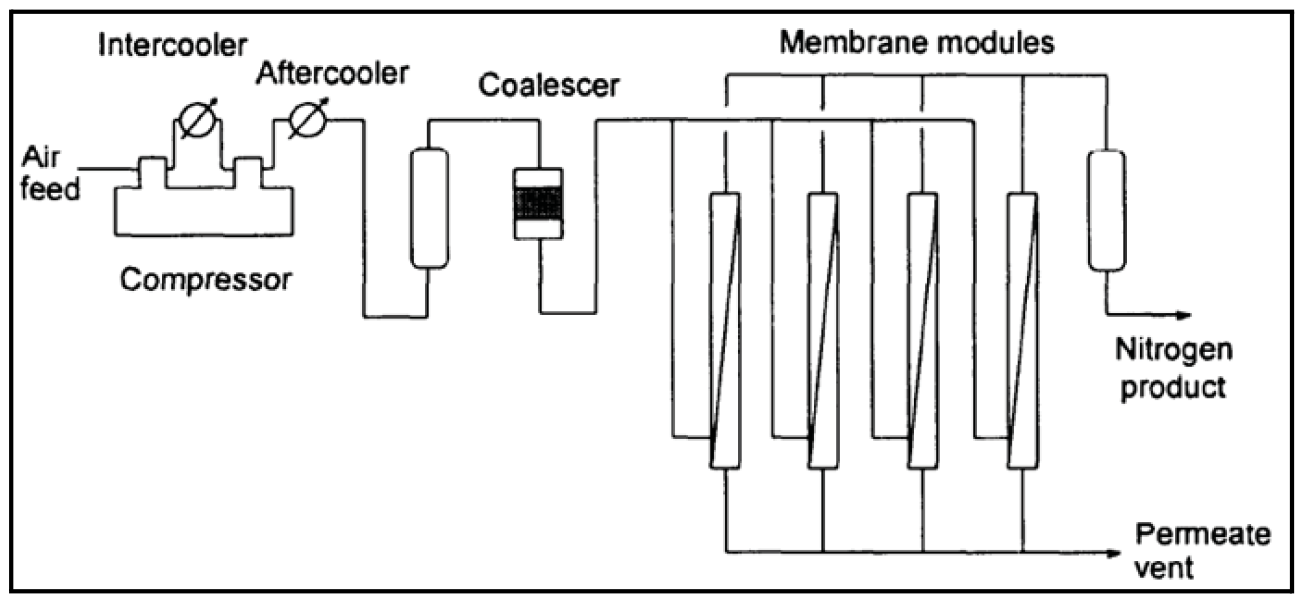
\includegraphics[scale=.5]{Figs/Fig9.png}
	\caption{Hệ thống tạo nitơ màng\cite{rehm2013underbalanced}}
	\end{figure}
	Hiệu suất của hệ thống tạo nitơ màng (hình 8)  thường là 50\%. Áp suất đầu vào hệ thống màng thường là 350 psi, đầu ra của máy nén khí là 300 psi. Nếu áp suất đầu vào tăng thì hiệu suất của hệ thống sẽ tăng, nhưng hiệu suât của bình và lượng oxi được giữ lại sẽ giảm. Màng nitơ thường khá nhậy cảm với nhiệt độ vì vậy trong hệ thống thường có thêm một bộ biến nhiệt. 
	\subsubsubsection{Ưu điểm}\\
		Vì hàm lượng oxi thấp nên khi đi vào bình tách kín nitơ màng khó bị kích thích cháy từ tĩnh điện.\\
		Nitơ màng có thể được sử dụng với dung dịch khoan gốc dầu. Không giống như khí tự nhiên, màng nitơ ít bị hòa tan trong dầu và ít gây ăn mòn hóa học cho hệ thống khoan.
	\subsubsubsection{Hạn chế}\\
		Chi phí sản xuất nitơ màng thương khá đắt đỏ vì hiệu suất của hệ thống sản xuất chỉ nằm vào khoảng 50\%, muốn tăng hiệu suất hệ thống thường phải tăng gấp đôi chi phí so với khi sử dụng các loại khí khác.
\subsubsection{Nitơ lỏng}
	Nitơ lỏng\cite{rehm2013underbalanced} là nitơ nguyên chất được hóa lỏng dưới nhiệt độ -320$^oF$. Nitơ lỏng được vận chuyển đến giàn khoan bằng xe bồn ở trên đất liền, bằng xà lan hoặc bình chứa ở trên biển.\\
	Nitơ được bơm bằng một loại bơm đặc biệt bơm ba bittong với áp suất lên tới 10000 psi hoặc hơn. Sau khi đi qua bơm, nitơ lỏng được gia nhiệt để trở về trạng thái khí hóa lỏng cho mục đích sử dụng.\\
	Nitơ có nhiệt dung riêng thấp, cần khoảng 134000 BTU để có thể sản xuất được 10000 scf khí nitơ từ nitơ ở trạng thái lỏng. Lượng nhiệt này thường có sẵn ở xe vận chuyển, ở những vùng có khí hậu lạnh cần phải dùng tới máy gia nhiệt để có thể cung cấp đủ nhiệt lượng cho việc sản xuất khí nitơ.
	\subsubsubsection{Ưu điểm}\\
	Không gây ăn mòn hóa học lên hệ thống khoan: \\
	Nitơ lỏng không chứa oxi vì vậy không hình thành nên môi trường ăn mòn. Tuy nhiên, nó vẫn có khả năng gây ăn mòn ở phần đáy giếng nếu xuất hiện sự có mặt của $CO_2$ và $H_2S$.\\
	Không gây cháy nổ:\\
	Nitơ lỏng nguyên chất không thể làm nguồn gây nổ hay cháy do nó không chứa oxi.Ngoài ra nitơ lỏng có thể hoặc động như một chất chống cháy.\\
	Áp suất cao:\\
	Nitơ có thể được bơm xuống dưới giếng với một áp suất rất lớn do quá trình hóa lỏng đã tạo ra một áp suất cực lớn trước đó. Vì vậy nitơ khá lí tưởng cho kỹ thuật khoan bằng khí.
	\subsubsubsection{Hạn chế}\\
	Giá thành:\\
	Hệ thống vận chuyển nitơ lỏng thường rất tốn kém, nitơ lỏng cần phải được chưa trong một loại bình chứa đặc biệt, cần được tăng áp và làm nóng trong quá trình vận chuyển. Chi phí vận chuyển thường nhiều hơn ít nhất gấp năm lần chi phí nén khí và ít nhất gấp hai lần chi phí sản xuất nitơ màng.\\
	Dễ bay hơi:\\
	Nitơ lỏng thường dễ bị bay hơi ở môi trường có nhiệt độ cao, trong quá trình vận chuyển đến giàn khoan.\\
	Chất chống cháy:\\
	Sự có mặt của khí nitơ làm hạn chế sự cháy trong hệ thống cháy. Vì vậy, cần phải có một lượng khá lớn khí tự nhiên để có thể không làm gián đoạn hệ thống cháy.
\subsection{Kỹ thuật khoan bằng Gaseated Fluid}
\subsubsection{Tổng quan}
	Gaseated fluid\cite{rehm2013underbalanced} là loại dung dịch khoan có khả năng thay đổi tỉ trọng một cách linh hoạt, là hỗn hợp giữa khí và lỏng mà không có thêm bất cứ một thành phần phụ nào khác như phụ gia tạo nhũ tương hay phụ gia tạo độ ổn định. Hệ thống gaseated được vận hành một cách rất dễ dàng, pha lỏng chỉ cần là một trong những dung dịch có khả năng tương thích vơi hệ thống khoan cả trong khi đóng giếng và mở giếng. Ở pha khí có thể dử dụng khí tự nhiên, nitơ hoặc những khí khác. Việc lựa chọn chất lưu sẽ phụ thuộc và tính chất của hệ thống (khả năng ức chế, độ bền nhiệt, mức độ nhiễm bẩn). Quá trình lựa chọn khí dựa trên mức độ nguy hiểm của khí đó khi ở trên mặt đất, down-holw fire, mức độ ăn mòn hóa học, giá thành và mức độ tiện lợi (ở gần hay xa giàn khoan).
\subsubsection{Dự đoán áp suất thủy tĩnh}
	Thể tích dung dịch bơm vào giếng có thể được thay đổi một cách linh hoạt khi sử dụng hệ thống gaseated. Tốc độ và thể tích dung dịch mong muốn phụ thuộc vào áp suất thủy tĩnh và tỉ trọng dung dịch tương đương ở phần trên của giếng. Sử dụng tỉ trọng dung dịch tương đương để tăng vận tốc dung dịch ở phần trên của giếng thường không thích hợp đồng thời còn phải phụ thuộc vào chu vi dính ướt và diện tích của khoảng không vành xuyến.\\
	Poettman và Bergman đã phát triển một mô hình dự đoán áp suất thủy tĩnh cho dung dịch gaseated ở điều kiện tĩnh. Hạn chế của phương pháp này là xét đến những điều kiện như ma sát hay ảnh hưởng của sự phân tách dung dịch trong khoảng không vành xuyến.\\
	Để dự đoán áp suất đáy giếng trong khi khoan bằng gaseated có thể sử dụng những mô hình tương quan dự đoán áp suất như tương quan Hagedorn - Brown, tương quan Beggs - Brill\cite{rehm2013underbalanced}. Nếu hệ thống gaseated được giả sử như là một hệ đồng nhất, có thể sử dụng định luật hàm mũ cho hỗn hợp khí-lỏng để tính toán tổn thất áp suất do ma sát trong khoảng không vành xuyến như sau:
	\begin{equation}
	\Delta P = \Delta L f \rho V_a^2/\{21.1(D_h-D_p)\}
	\end{equation}
	Với
	\begin{enumerate}
		\item[] $f$ = Hệ số ma sát đạt được bằng cách tính toán hệ số Reynolds
		\item[] $\delta P$ = Tổn thất áp suất do ma sát, psi
		\item[] $\delta L$ = Chiều dài ước lượng, ft
		\item[] $\rho$ = Tỉ trọng dung dịch, ppg
		\item[] $\nu_a$ = Độ nhớt dẻo của dung dịch
		\item[] $V_a$ = Tốc độ trung bình trong khoảng không vành xuyến, ft/sec
		\item[] $D_h$ = Đường kính giếng khoan, in
		\item[] $D_p$ = Đường kính chuỗi cần khoan, in.
	\end{enumerate}
\subsubsection{Giới hạn thể tích khí và thể tích dung dịch}
	\subsubsubsection{Giới hạn thể tích khí}\\
	Trong hệ thống gaseated, pha lỏng thường là pha liên tục. Lượng khí trong dung dịch bị giới hạn ở mức khoảng 80\% thể tích dung dịch để tránh hiện tượng áp suất tăng đột ngột dẫn tới mất khả năng vận chuyển mùn khoan ở gần bề mặt.\\
	Tăng thể tích khí trong dung dịch sẽ tăng tốc độ của dung dịch thế chỗ làm cho áp suất ma sát lớn hơn áp suất sụt giảm trong quá trình bơm thêm khí.
	\subsubsubsection{Giới hạn thể tích dung dịch}\\
	Dung dịch được bơm xuống giếng qua cần khoan để làm mát chòong khoan và làm chạy động cơ đáy. Sử dụng dung dịch khoan là phương pháp cơ bản nhất để làm sạch giếng. Giới hạn dưới của thể tích dung dịch:
	\begin{itemize}
		\item Khả năng làm sạch giếng
		\item Vận hành động cơ đáy.
	\end{itemize}
	
	Giới hạn trên của thể tích dung dịch:
	\begin{itemize}
		\item Chế độ ưu thế ma sát
		\item Vận hành động cơ đáy.
	\end{itemize}
	
	Trước khi khoan vào một vùng xác định sử dụng kỹ thuật khoan bằng gaseated fluid cần phải xem xét các thông số áp suất vỉa, giới hạn của động cơ đáy, khả năng vận chuyển mùn khoan và mức độ ổn định thành giếng. Dòng chảy phải được giới hạn trong vùng ưu thế ma sát để có thể vận hành trơn tru hơn. 
\subsubsection{Ưu điểm}
Hệ thống gaseated mang lại nhiều ưu điểm như đơn giản, linh động vì vậy kỹ thuật này thường được lựa chọn để giảm áp suất đáy giếng. Giảm áp suất đáy giếng có thể loại bỏ được những vấn đề như mất dung dịch tuần hoàn, kẹt cần do chênh lệch áp suất đồng thời còn có thể đẩy nhanh tốc độ khoan, giảm thiệt hại đến thành hệ. \\
	\subsubsubsection{Bảo vệ vỉa}\\
	Khoan bằng gaseated fluid được xem là một kỹ thuật khoan có khả năng bảo vệ vỉa tốt nhất bởi, giảm được những thiệt hại lên thành hệ trong quá trình khoan. Đồng thời kỹ thuật này cũng loại bỏ hoặc giảm thiểu những vấn đề liên quan đến việc dung dịch khoan đi vào thành hệ. 
	\subsubsubsection{Loại bỏ hoặc làm giảm mất dung dịch}\\
	Bằng cách ngăn chặn mất mát dung dịch trong khi tuần hoàn, hệ thống gaseated được ứng dụng vào công nghiệp dầu khí để loại bỏ khoảng thời gian không sinh lợi.
	\subsubsubsection{Loại bỏ vấn đề kẹt cần do chênh lệch áp suất}\\
	Kẹt cần do chênh lệch áp suất là kết quả của việc lớp mud cake và áp suất dư trong khoảng không vành xuyến. Trong kỹ thuật khoan bằng gaseated fluid, áp suất trong khoảng không vành xuyến nhỏ hơn áp suất thành hệ vì vậy loại trừ được những điều kiện xảy ra kẹt cần.
	\subsubsubsection{Tăng tốc độ khoan và tuổi thọ của chòong khoan}\\
	Khi áp suất đáy giếng lớn hơn áp suất thành hệ, mùn khoan sẽ bị giữ lại ở đáy giếng(chip hold down pressure), hiện tượng này làm tăng thời gian làm sạch giếng. Khoan bằng hệ thống gaseated loại bỏ hiện tượng chip hold down pressure và tăng tốc độ khoan.\\
	Tuổi thọ của chòong khoan cũng được tăng đáng kể so với kĩ thuật khoan truyền thống. Áp suất đáy giếng thấp, lực tác động lên chòong khoan giảm, ứng suất ma sát tạo ra bởi các hạt rắn giảm đồng thời trọng lượng lên chòong giảm vì vậy có thể tăng nhanh tốc độ khoan và tuổi thọ chòong khoan, điều này làm giảm những chi phí phát sinh không đáng có. 
	\subsubsubsection{Đánh giá vỉa}\\
	Trong quá trình khoan dưới cân bằng, vỉa có tiềm năng dầu khí có thể được phát hiện ngay sau khi khoan vào tầng vỉa bằng cách đo đạt và theo dõi sự thay đổi của dung dịch khoan tại ống tháo cạn hoặc sau bình tách. Dung dịch trong vỉa có thể được kiểm soát trên bề mặt bằng cách xác định những vỉa có tiềm năng dầu khí. Quá trình thử vỉa được thực hiện trong khi khoan để có thể xác định được tiềm năng dầu khí của vỉa.
	%\clearpage
	\begin{figure}[h]
		\centering
		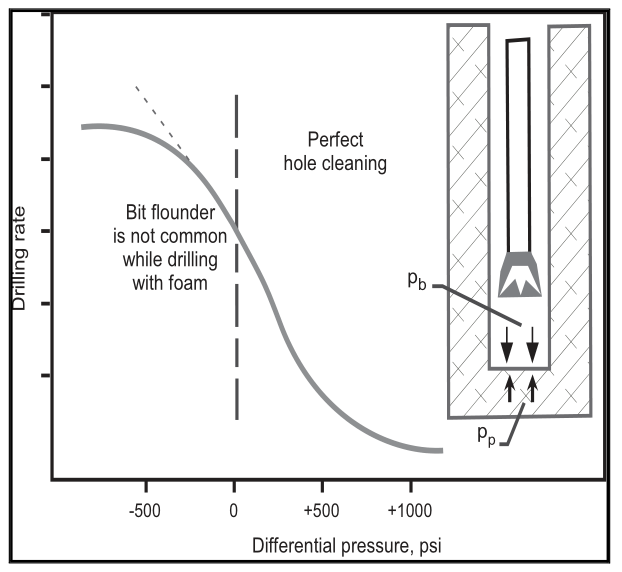
\includegraphics[scale=0.5]{Figs/Fig11.PNG}
		\caption{Tốc độ khoan và áp suất đáy giếng\cite{rehm2013underbalanced}}
	\end{figure}
\subsubsection{Hạn chế}
	\subsubsubsection{Giá thành}\\
	Gaseated drilling thường có giá thành cao hơn so với các phương pháp khoan truyền thống, đặc biệt là khoan ở những vị trí khắc nhiệt như trên biển hay trong sa mạc. So với khoan truyền thống, khoan bằng gaseated fluid còn cần phải có thiết bị kiểm soát khoan xoay, máy nén, bình tách, bình chứa, nhân lực và các chi phí phát sinh trong khi khoan. 
	\subsubsubsection{Pressure surges}\\
	Hệ thống gaseated thường không ổn định. Khi pha khí trong dung dịch đi lên tới bề mặt và thoát ra ngoài thông qua đường tiết lưu. Pha lỏng sẽ bị nén xuống dưới làm tăng áp suất đáy giếng và giữ pha khí bên trong cột chất lỏng bị nén. Khi cột dung dịch này được tuần hoàn thông qua đường tiết lưu và làm giảm áp suất trong giếng, quá trình này được lặp đi lặp lại nhiều lần mỗi hai mươi phút tạo ra hiện tượng pressure surges.\\
	Pressure surges thường gây ra những thiệt hại lớn lên thành hệ, làm giảm khả năng ổn định của thành giếng. Hiện tượng này có thể được kiểm soát trong khi khoan bằng cách kết hợp các phương pháp kiểm soát khoan xoay, vận tốc dung dịch, đối áp bề mặt để có thể thay đổi tính chất dòng tuần hoàn ngược.\\
	Ngoài ra, để hạn chế hiện tượng pressure surges tại các vị trí kết nối, có thể bơm thêm khí vào trong giếng trước khi kết nối để làm khô phần trên của cần khoan. Sau quá trình kết nối, phải giảm được khí được bơm vào để có thể loại bỏ pressure surges.
	%\clearpage
	\begin{figure}[h]
	\centering
	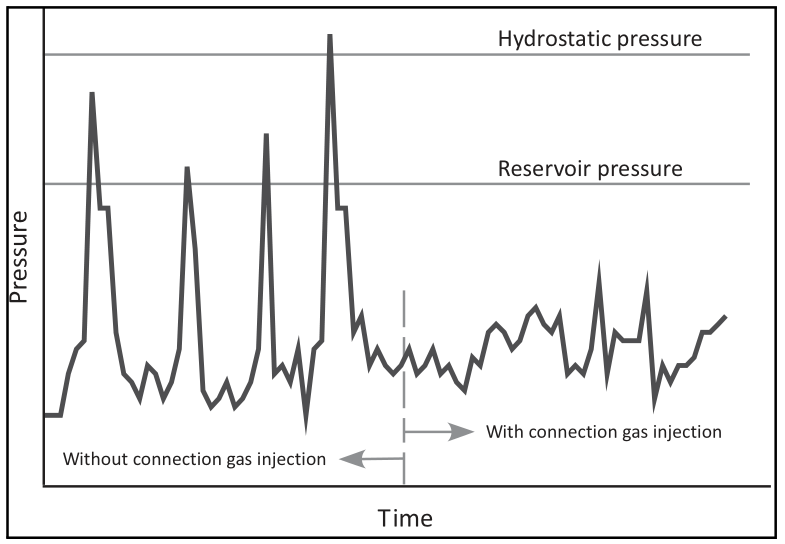
\includegraphics[scale=0.5]{Figs/Fig12.PNG}
	\caption{Tối ưu lượng khí bơm vào hệ thống tuần hoàn trước khi kết nối\cite{rehm2013underbalanced}}
	\end{figure}
	\subsubsubsection{Một số hạn chế khác}\\
		\begin{itemize}
			\item Nứt vỡ: Khi xuất hiện những nứt vỡ lớn trong giếng, dung dịch đi vào trong nứt vỡ gây ra hiện tượng mất dòng liên tục ở mức thấp, điều này dễ làm cho giếng bị kick tại những vị trí kết nối. Nguyên nhân chính của vấn đề này là do trọng lực làm thay đổi dòng dung dịch và dòng tuần hoàn khi tắt bơm dung dịch.
			\item Sự hấp thụ: Lực mao dẫn trong vỉa có thể gây ra hiện tương hấp thụ dung dịch khoan, dung dịch bị hút vào trong vỉa kể cả khi giếng đang sử dụng phương pháp khoan dưới cân bằng. Để giảm thiểu lượng dung dịch bị hút vào trong vỉa, áp suất trong khoảng không vành xuyến cần phải nhỏ hơn áp suất thành hệ gây ra bởi áp suất mao dẫn và pha lỏng của dung dịch khoan phải hạn chế được sự dính ướt lên thành hệ.
			\item Ngừng tuần hoàn: Ngừng tuần hoàn có thể dẫn dến hư hại thành hệ hoặc giảm hiệu suất của dung dịch do mất mát dung dịch.
		\end{itemize}
\subsection{Flow-drilling (Drilling mud)}
	\subsubsection{Tổng quan về hệ thống dung dịch khoan đơn pha}
	Sử dụng hệ thống dung dịch khoan đơn pha (Flow drilling)\cite{rehm2013underbalanced} trong khoan dưới cân bằng không phải là một phương pháp mới hay đặc biệt, tạp chí API Journals ghi nhận đưa vào sử dụng từ những năm 1930. \\
	\begin{figure}[h]
		\centering
		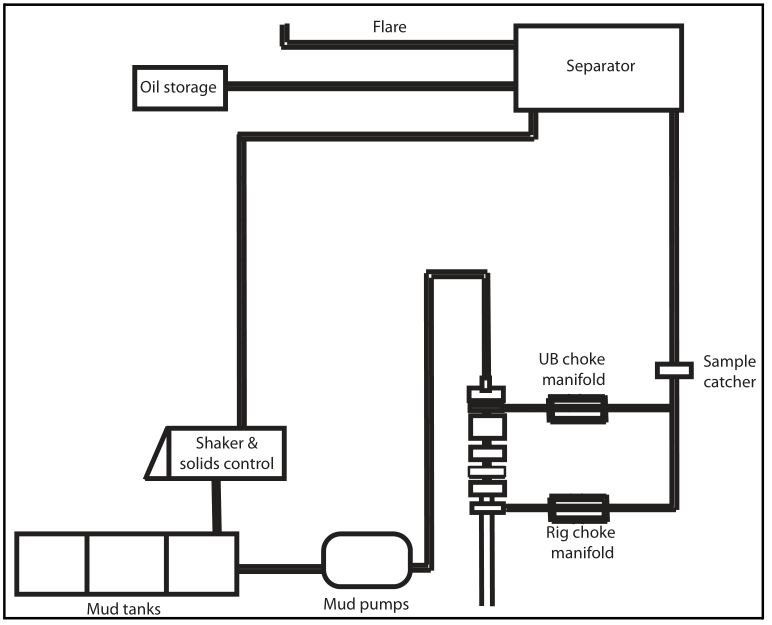
\includegraphics[scale=0.5]{Figs/Fig18.PNG}
		\caption{Flow drilling\cite{rehm2013underbalanced}}
	\end{figure}
	Sử dụng flow drilling trong những vỉa có độ thấm thấp, áp suất vỉa cao được coi là phương pháp tối ưu mang lại nhiều lợi ích về mặt kinh tế do khả năng tăng nhanh tốc độ khoan trong thành hệ bất ổn định. Hiện nay, nhiều hệ thống sử dụng dung dịch khoan từ nước nguyên chất hay nhũ tương ngược để có thể giảm tỉ trọng dung dịch xuống mức thấp nhất đồng thời tăng áp suất bề mặt tại choke để bù cho áp suất mất mát do giảm tỉ trọng dung dịch.\\
	Những thay đổi về tính chất dung dịch có thể cho biết những thay đổi về áp suất (từ áp suất dưới cân bằng sang áp suất cân bằng), chỉ ra những vùng gây mất dung dịch. Khi xảy ra sự thay đổi này, có thể sử dụng flow drlling để giải quyết vấn đề.
	\subsubsection{Lợi ích khi sử dụng dung dịch khoan đơn pha}
	Bên cạnh khả năng tăng tốc độ khoan, sử dụng dung dịch khoan đơn pha giúp làm giảm mất mát dung dịch trong khi khoan, giảm hư hại thành hệ và ngăn chặn hoặc giảm thiểu kẹt cần do chênh áp.
		\subsubsubsection{Hệ thống đơn giản}\\
		Dung dịch khoan đơn pha không yêu cầu một hệ thống phức tạp trong khi dung dịch khoan bọt, đa pha hay gaseated đều có những khó khăn trong quá trình vận hành hệ thống đồng thời tốn nhiều chi phí. Mô hình lưu biến đơn giản. Trong khi vận hành dễ dàng kiểm soát những thay đổi tỉ trọng dung dịch tương đương, ECD, (những thay đổi này thường xảy ra khi di chuyển cần khoan ra vào giếng và thay đổi tốc độ bơm) hơn so với việc phải dự đoán và kiểm soát hệ dung dịch đa pha. Dễ dàng thực hiện kiểm soát áp suất giếng và theo dõi chế độ áp suất đáy giếng.
		\subsubsubsection{Chi phí thấp}\\
		Chi phí cho việc sử dụng khí và máy nén khí được loại bỏ do sử dụng dung dịch đơn pha.
		\subsubsubsection{Có thể sử dụng động cơ đáy và các thiết bị đo trong khi  khoan truyền thống} \\
		Do không có pha khí trong cần khoan, động cơ đáy những thiết bị trong phương pháp khoan truyền thống có thể được sử dụng để thực hiện MWD, LWD và PWD.
		\subsubsubsection{Tăng tốc độ khoan}\\
		Dung dịch khoan ảnh tác động mạnh nhất đến hai yếu tố:
		\begin{itemize}
			\item Độ giòn của đất đá (thường tăng)
			\item Khả năng rửa trôi mùn khoan khỏi đáy giếng (thường tăng)
		\end{itemize}
		Do khả năng làm sạch đáy giếng tốt và xu hướng làm tăng độ giòn của đất đá, khi kết hợp với choòng khoan ba chóp xoay tốc độ khoan thường được tăng đáng kể. 
		\subsubsubsection{Giảm mất mát dung dịch tuần hoàn}\\
		Lần đầu tiên khoan dưới cân bằng sử dụng dung dịch khoan đơn pha được áp dụng là để tránh mất dung dịch trong khi khoan. Đến nay, đây vẫn là một trong những lợi ích cơ bản khi xem xét sử dụng dung dịch khoan đơn pha. Cách tốt nhất để tránh mất dung dịch là giữ cho giá trị ECD nhỏ hơn giá trị áp suất vỡ vỉa hoặc nhỏ hơn áp suất thành hệ trong trường hợp vỉa có độ thấp cao, vỉa có nhiều nứt nẻ. 
		\subsubsubsection{Giảm kẹt cần do chênh áp}\\
		Kẹt cần do chênh áp thường xảy ra do sự xuất hiện lớp filter cake (quá dày) và áp suất giếng lớn hơn áp suất thành hệ. Khi sử dụng dung dịch khoan đơn pha kết hợp với phương pháp khoan dưới cân bằng có thể loại bỏ được lớp filter cake, đồng thời áp suất thành hệ cũng lớn hơn áp suất trong giếng. Vì vậy có thể hạn chế được kẹt cần do chênh áp.
		\subsubsubsection{Giảm hư hại thành hệ}\\
		Trọng khi khoan áp suất trong giếng nhỏ hơn áp suất thành hệ, dòng chảy trong khoảng không vành xuyến không đi vào thành hệ. Do đó những hư hại gây ra bởi dung dịch khoan và mùn khoan rắn được hạn chế.
		\subsubsubsection{Thực hiện thử vỉa trong khi khoan}\\
		Cho phép kiểm tra dòng vào để có thể thực hiện thử vỉa trước khi chống ống hoặc trám xi măng. Khi thử vỉa cần đo chính xác những thông số áp suất và dòng do đó cần những thiết bị đo đặc biệt phù hợp với khoan dưới cân bằng.
	\subsubsection{Giới hạn}
		\subsubsubsection{Độ ổn định thành hệ}\\
		Khó khăn lớn nhất thường gặp trong khoan dưới cân bằng là những tính chất địa chất liên quan đến độ ổn định thành hệ.
			\begin{figure}[h]
				\centering
				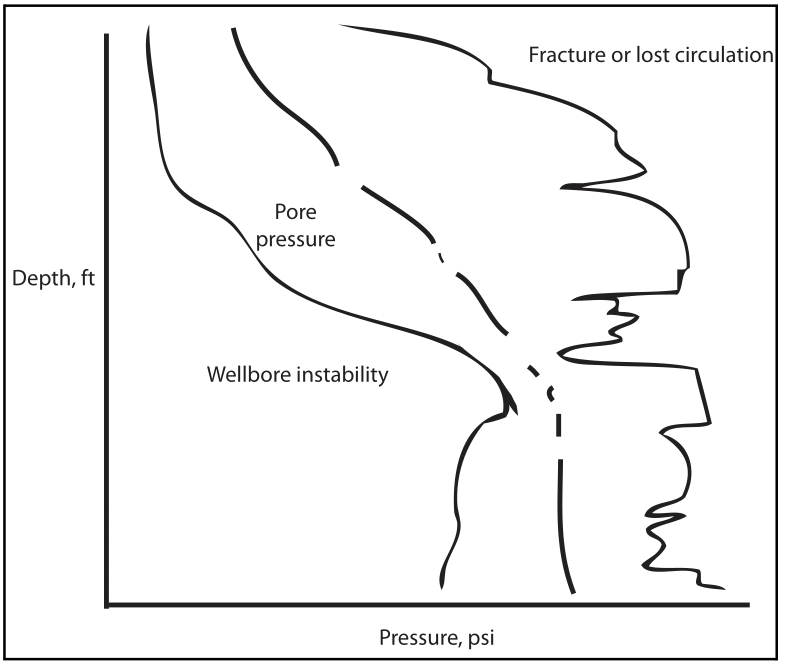
\includegraphics[scale=0.6]{Figs/Fig19.PNG}
				\caption{Độ ổn thành giếng theo áp suất thành hệ\cite{rehm2013underbalanced}}
			\end{figure}
		\subsubsubsection{Độ thấm đứt gãy và lưu lượng dòng trong vỉa}\\
		Dòng chất lưu trong vỉa có mối liên quan chặt chẽ đến quá trình vận hành khoan dưới cân bằng, là một trong những tiêu chí quan trọng để lựa chọn kĩ thuật khoan, HSE và hệ thống bình tách. Trong những vùng có đứt gãy hoặc độ thấm lớn, việc duy trì dung dịch tuần hoàn rất khó khăn trong cả giếng đứng và giếng ngang. Phương pháp khoan mud cap thường được sử dụng cho những vùng có điều kiện địa chất này.
		\subsubsubsection{Khí H\texorpdfstring{$_2$}{2}S}\\
		Sự xuất hiện của khí H$_2$S trong khi khoan gây ra nhiều vấn đề về môi trường. Mặc dù có thể được xử lý để không ảnh hưởng tại khu vực giàn khoan, nhưng những vùng cư dân lân cận thường bị ảnh hưởng do H$_2$S phát tán trong không khí.

\section{Các vấn đề thường gặp trong khoan dưới cân bằng}
\subsection{Hệ thống Coiled Tubing}
\subsubsection{Tổng quan}
	Coiled tubing\cite{rehm2013underbalanced} là một thiết bị đặc biệt và đang ngày càng thay đổi với với công nghệ tiên tiến hơn. Coiled tubing thường có những vấn đề liên quan tới kích thước, quá trình gia công và khả năng sử dụng trong hệ thống khoan xoay thấp. Đã có nhiều thay đổi trong việc lựa chọn vật liệu và kĩ thuật trong quá trình gia công, vì vậy những vấn đề này đang dần được hạn chế. \\
	Những hạn chế về khả năng khoan xoay của coiled tubing dẫn đến các vấn đề về momen xoắn và khả năng làm sạch giếng, đặc biệt là trong những giếng khoan định hướng có góc ngiêng lớn. Để xử lý những vấn đề liên quan đến momen xoắn, hệ thống khuấy và hệ thống kéo được phát triển. Tuy nhiên,khả năng làm sạch giếng vẫn là một vấn đề gây đau đầu, mặc dù có thể thay đổi tính chất dung dịch khoan để có thể cải thiện mức độ làm sạch giếng.\\
	Những ưu điểm và hạn chế của hệ thống coiled tubing (Bảng 1):
	\begin{table}[h]
	\centering
	\caption{Ưu điểm và hạn chế của coiled tubing\cite{rehm2013underbalanced}}
	\label{Table}
	\begin{tabular}{|c|c|}
	\hline
	\rowcolor[HTML]{C0C0C0} 
	 \textbf{Ưu điểm} & \textbf{Hạn chế} \\ \hline
	 Khoan cho giếng thân nhỏ  &Khả năng cứu kẹt thấp   \\ \hline
	 Lắp đặt nhanh & Tốn thời gian lắp đặt BHA  \\ \hline
	 Không cần sử dụng tool joints cho BHA & BHA tốn nhiều chi phí  \\ \hline
	 Tốn ít thời gian vận chuyển & Giàn tốn nhiều chi phí  \\ \hline
	 Hệ thống áp suất linh hoạt & Áp suất bơm ép khí quá cao, cần sử dụng Nitơ lỏng \\ \hline
	 Đã khoan thành công ở nhiều giếng & Không tối ưu được chi phí trong nhiều trường hợp  \\ \hline
	 Thực hiện MWD nhanh hơn & BHA khó thay thế  \\ \hline
	 Hệ thống dịch vụ nhanh gọn & BHA không thể xử lý được nhiều loại dung dịch  \\ \hline
	 Dễ dàng HSE & Tuổi thọ tubing thấp  \\ \hline
	 Đội ngũ nhân lực có nhiều kinh nghiệm &  Thiếu nguồn nhân lực tay nghề cao  \\ \hline
	 Sử dụng được nhiều loại dung dịch khoan & Thiếu nguồn vật tư kĩ thuật  \\ \hline
	  & Tốn nhiều chi phí khi xảy ra sự cố  \\ \hline
	  & Khả năng giữ cần nặng và ống chống kém  \\ \hline
	  & Nhậy cảm với ăn mòn hóa học  \\ \hline
	\end{tabular}
	\end{table}
	\subsubsection{Hệ thống thiết bị}
	\subsubsubsection{Bơm ép coiled tubing}
	Đầu bơm ép coiled tubing cung cấp một công suất cần thiết đủ để có thể đẩy hoặc kéo coiled tubing vào hoặc ra khỏi giếng. Hệ thống thủy lực cho phép kiểm soát coiled tubing và chuỗi cần khoan ở mức độ cao, điều này ảnh hưởng rất lớn đến tải trọng lên choòng . Chức năng cơ bản của đầu bơm ép là tác động một lực dọc trục lên coiled tubing để có thể kiểm soát chuyển động của coiled tubing trong giếng, cung cấp một lực thích hợp để kéo tubing không bị tụt xuống dưới, tác động một lực không đổi khi tubing đang ở trạng thái trung hòa và đồng thời hoạt động như một cảm biến đo độ sâu. 
	\subsubsubsection{Cổ ngỗng}
	Cổ ngỗng được đặt trên đầu của đầu bơm ép, coiled tubing được định hướng từ hệ thống cuộn tới đầu bơm ép thông qua cổ ngỗng. Trục lăn trên đầu cổ ngỗng cho phép tubing vận hành trơn tru hơn.
	\subsubsubsection{Hệ thống cuộn}
	Chức năng chính của hệ thống cuộn là làm nơi lưu trữ và bảo vệ chuỗi coiled tubing. Thiết kế của hệ thống cuộn được tối ưu cho từng môi trường hoạt động như trên biển hoặc trên đất liền.\\
	Hệ thống cuộn được kết nói với hệ thống thủy lực để có thể vận hành một cách chính xác nhất. Mặc dù có thể sử dụng hệ thống cơ để điều khiển nhưng cần có thêm một số thiết bị kiểm soát độ bền, đường kính và độ uốn của tubing. \\
	Hệ thống cuộn có dây điện được lắp đặt thêm vách ngăn áp suất và bộ thiết bị góp. Thiết bị góp được đặt cuối đường dây điện để có thể kết nối với các thiết bị bề mặt. Đường dây điện kết nối và dẫn điện tới các thiết bị lòng giếng và các thiết bị MWD, đồng thời cũng truyền tín hiệu đo được từ các thiết bị lòng giếng lên trên bề mặt. Vách ngăn áp suất có nhiệm vụ tạo màng chắn áp suất xung quanh các đường dây tín hiệu, cho phép dung dịch khoan được bơm vào phâng còn lại của tubing mà không ảnh hưởng đến đường truyền tín hiệu. \\
	Áp suất bề mặt ảnh hưởng đến khả năng tải tubing của hệ thống cuộn hay chiều dài thực tế của coiled tubing, áp suất càng tăng thì tubing càng dài. Tuy nhiên, sự thay đổi này thường không tuyến tính do tổn thất áp suất quá trình chuyển từ trạng thái cuộn quanh hệ thống cuộn sang trạng thái thẳng khi được đưa xuống giếng thường rất lớn. \\
	\begin{figure}[h]
	\centering
	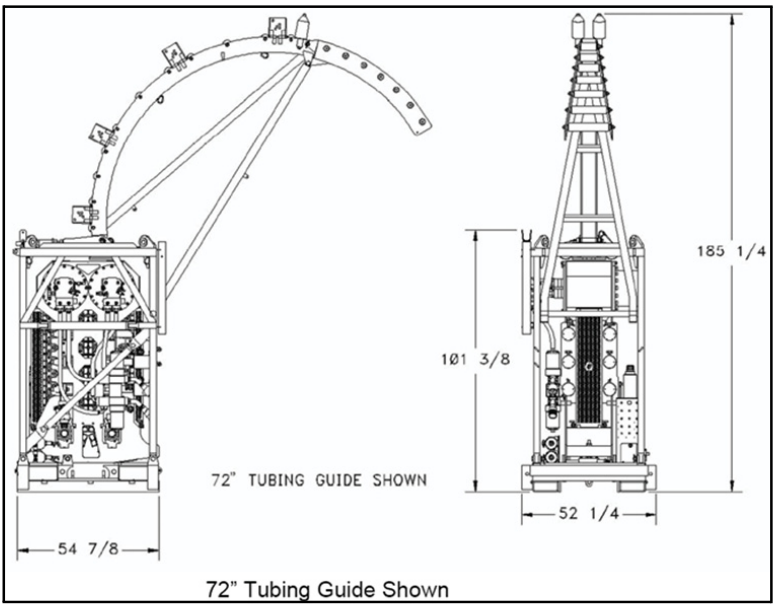
\includegraphics[scale=.7]{Figs/Fig14.PNG}
	\caption{Cổ ngỗng và đầu bơm ép\cite{rehm2013underbalanced}}
	\end{figure}
	\newpage
	Mức tải tubing của hệ thống cuộn thường được tính theo công thức sau:
	\begin{equation}
	L = (A + C)ABK
	\end{equation}
	Trong đó:
	\begin{enumerate}
		\item[] L = Mức tải tubing, ft
		\item[] A = Chiều cao của tubing stack, in
		\item[] B = Khoảng cách giữa hai mặt bích, in
		\item[] C = Đường kính trong của hệ thống cuôn, in
		\item[] K = Hằng số kích thước của mỗi loại tubing, $ft/in^3$
	\end{enumerate}
	\begin{figure}[h]
	\centering
	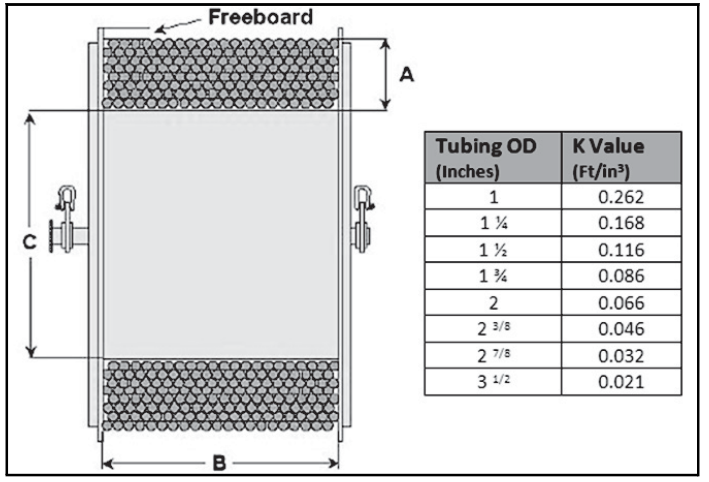
\includegraphics[scale=.7]{Figs/Fig15.PNG}
	\caption{Mức tải tubing\cite{rehm2013underbalanced}}
	\end{figure}
	\subsubsubsection{Phòng điều hành}
	Trong khi thực hiện công việc coiled tubing(từ lắp đặt, vận hành đến tháo dỡ) cần có một phòng điều hành nhỏ để có thể kiểm soát các thông số của đầu bơm ép, BOP, hệ thống cuộn và là nơi hiển thị, lưu trữ dữ liệu. Trong khoan định hướng bằng coiled tubing, cần phải có một phòng điều hành lớn để tạo được sự thuận lợi và thoải mái nhất có thể khi hoạt động trong thời gian dài.
	\subsubsection{Hệ thống kiểm soát giếng}
	Lựa chọn, thiết kế hệ thống kiểm soát giếng khoan bằng coiled tubing dựa trên những yếu tố sau:
	\begin{itemize}
		\item Trường hợp xấu nhất có thể xảy ra với giếng
		\item Nhà điều hành (Exxon, BP, Shell,...)
		\item Đề xuất thông qua kinh nghiệm thực tế.
	\end{itemize}
	Trước khi lắp đặt hệ thống kiểm soát giếng cho giếng khoan bằng coiled tubing cần phải xem xét lại các tài liệu trong quá trình khoan trước đó để có thể tối ưu hóa được thiết kế của hệ thống. Khi lập kế hoạch khoan, BOP phải đảm bảo được chức năng xử lý các vấn đề về áp suất được giữ trên và dưới ram đơn, cho phép cân bằng áp suất tại miệng giếng trong quá trình khoan.
	\clearpage
	\begin{figure}[h]
	\centering
	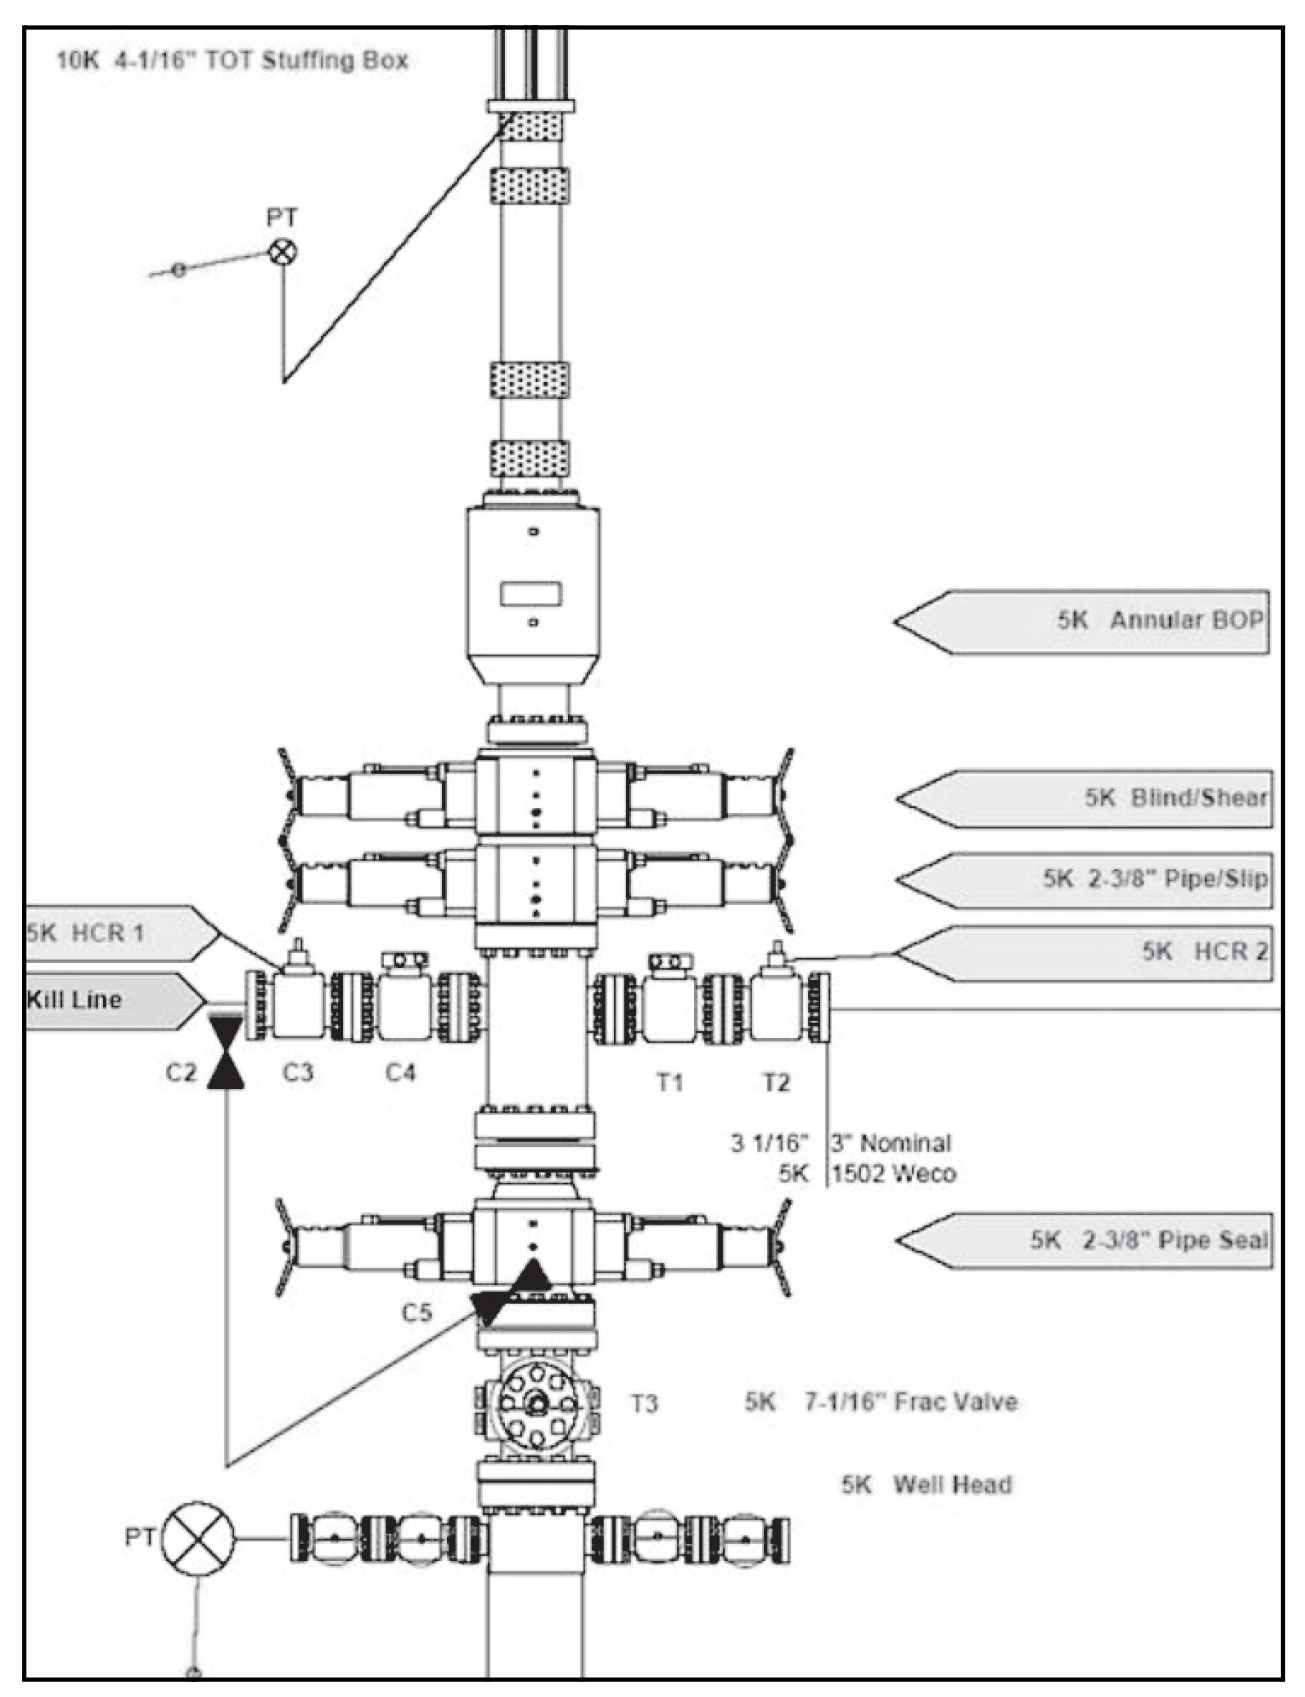
\includegraphics[scale=.3]{Figs/Fig16.png}
	\caption{Hệ thống BOP\cite{rehm2013underbalanced}}
	\end{figure}
	%\newpage
	\subsubsubsection{Hệ thống dầu bôi trơn}
	Khi thực hiện kéo thả bộ khoan cụ trong khoan bằng coiled tubing, áp suất cần phải được giữ dưới mức cân bằng. Hệ thống dầu bôi trơn bao gồm tời và các hợp chất dầu bôi trơn giúp giữ cho việc kéo thả bộ khoan cụ diễn ra thuận lợi, không gây ra các vấn đề ``surges'' hay ``swab''. 
	\subsubsubsection{Bộ khoan cụ}
	Hai nhà thầu dịch vụ phổ biến nhất cung cấp bộ khoan cụ cho coiled tubing là Baker Hughes với Baker Hughes Inteq và Halliburton với Sperry Sun. \\
	Bộ khoan cụ cần phải được lựa chọn và thiết kế thích hợp với mục đích, môi trường của giếng. Nếu trong trường hợp thiếu thiết bị bộ khoan cụ của Baker Hughes sẽ được đưa vào thay thế. Với khả năng tự động cao, khả năng chịu nhiệt tốt, Baker Hughes Inteq có thể sử dụng được cho nhiều giếng khoan trong môi trường khác nhau. Tuy nhiên, do mức độ linh hoạt và khả năng khoan trong giếng thân nhỏ làm cho Baker Hughes Inteq tiêu tốn nhiều kinh phí so với khoan truyền thống.
\subsubsection{Vận hành}
	Hai phương pháp vận hành coiled tubing thường thấy là vận hành trong thời gian dài và vận hành khẩn cấp. Trong vận hành khẩn cấp, đội ngũ nhân viên phải được tập luyện để có thể ứng phó với những trường hợp bất ngờ một cách nhanh nhất.\\
	Bơm ép khí trong coiled tubing cần áp suất rất cao, vì vậy cần phải chắc chắn rằng đường ống giữa bơm và ống dâng đã được lắp đặt, kiểm tra thường xuyên ở trên các đoạn nối, áp suất kiểm tra phải gấp 150\% so với áp suất vận hành trong đường ống.
	\subsubsubsection{Kiểm soát coiled tubing}
	Hệ thống coiled tubing cũng coi là một thiết bị khoan nhưng không giống cần khoan, tubing thường rất yếu, dễ dàng bị phá hủy, nhạy cảm với áp suất, nhiệt độ và những hoạt chất hóa học dùng trong khi khoan khác. Hiện nay có rất ít những hệ thống có thể kiểm tra trực tiếp được độ mỏi, độ uốn, và áp suất tác động lên tubing. Do đó, việc đo đạt được thực hiện bằng tay (gián tiếp) từ độ sâu, áp suất đến chu kì quay của tubing đẫn đến những kết quả về độ bền mỏi hay tuổi thọ của tubing chỉ mang tính chất định tính. Kể cả đối với những thiết bị khác, hư hại vẫn có thể xảy ra do lỗi của nhà sản xuất, lỗi của nhà vận hành và từ những vấn đề không dự đoán được. \\
	Kiểm soát tubing cần phải được thực hiện liên tục, ổn định. Sau khi khoan xong, dữ liệu trong quá trình khoan cần được gửi về trung tâm để phân tích tuổi thọ của coiled tubing đối với từng giếng, sau đó được lưu trữ vào hệ thống trung tâm.
	\subsubsubsection{Những vấn đề cần được thực hiện trong quá trình vận hành khoan}
	\begin{itemize}
		\item Kiểm soát hàm lượng hạt rắn và áp suất trong khi tuần hoàn dung dịch
		\item Thực hiện kiểm tra và báo cáo những hoạt động khoan về trung tâm mỗi ngày
		\item Không mở ECD trong giếng thân trần ngoại trừ trường hợp bắt buộc
		\item Kiểm tra đường kính trong và đường kính ngoài của các thiết bị lòng giếng cho quá trình thả thiết bị xuống giếng
		\item Kiểm tra các thiết bị MWD khi thả thiết bị xuống giếng để đảm bảo được chức năng của thiết bị
		\item Lựa chọn tải lên choòng và giảm áp suất đáy giếng.
		\item Lập báo cáo hàng ngày về thể tích và tầng số quét thông qua mùn khoan được mang lên bề mặt. Những thông tin này được sử dụng để tối ưu hóa tầng số và thể tích quét
		\item Theo dõi chặt chẽ mọi sự khác biệt về motor, trọng lượng của tubing trên bề mặt, tải trọng lên choòng và áp suất đáy giếng
		\item Thực hiện làm sạch mỗi trên tubing mỗi 300 ft, chỉ thay đổi tần suất khi điều kiện vỉa và thành giếng có sự thay đổi lớn. 
	\end{itemize}
\subsubsection{Thách thức}
	\subsubsubsection{Làm sạch giếng}
	Loại bỏ mùn khoan ra khỏi giếng rất quan trọng trong việc thay đổi trọng lượng lên choòng, giảm nguy cơ kẹt cần, đồng thời tối uy được điều kiện cho quá trình kéo thả ống ra vào giếng. Trong giếng khoan định hướng, dung dịch cần phải tăng độ nhớt để có thể nâng cao khả năng vận chuyển mùn khoan. Vận tốc bơm phải được giữa mở mức cao để có thể giữ cho vận tốc dung dịch trong khoảng không vành xuyến đạt mức chấp nhận sau khi tăng độ nhớt của dung dịch khoan. Khi mùn khoan bị tích tụ quá nhiều dưới đáy giếng, cần phải khuấy để dung dịch khoan có thể vận chuyển mùn khoan lên bề mặt. Hệ thống coiled tubing không thể xoay và không có tool joints, choòng khoan chỉ có thể khuấy lớp mùn khoan trong khi khoan phần thân trần, vì vậy wiper tríp cần phải được thực hiện định kì mỗi 150 ft để chắc chắn rằng mùn khoan đã được loại bỏ khỏi giếng.
	\subsubsubsection{Tốc độ khoan}
	Tốc độ khoan bị giảm khi có quá nhiều mùn khoan bị tích tụ dưới đáy giếng và do sự thay đổi của thành phần thạch học. \\
	Phương pháp xử lý:
	\begin{itemize}
		\item Đảm bảo rằng tốc độ khoan không bị giảm bởi những nguyên nhân cơ học 
		\item Đảm bảo rằng mọi sự thay đổi về thành phần thach học đều được xác định trước
		\item Nếu như nguyên nhân không đến từ các thay đổi về thạch học và nguyên nhân cơ khí, cần phải thực hiện wiper trips kiểm tra tải trọng lên choòng. Nếu tải trọng lên choòng ở mức bình thường, thả lại bộ khoan cụ vào giếng và tiếp tục khoan. Nếu tải trọng quá lớn cần phải thực hiện wiper trips 
		\item Thực hiện fullwiper trips nếu như phát hiện short wiper trips không đủ thể loại bỏ hết mùn khoan khỏi bộ khoan cụ.
	\end{itemize}
	\subsubsubsection{Wellhead và áp suất khoảng không vành xuyến}
	Khi áp suất trong khoảng không vành xuyến tăng, giếng dễ bị kick. Khi áp suất thay đổi liên tục (tăng hoặc giảm) trong một khoảng thời gian ngắn, giếng dễ bị ``Slugging''.\\
	Phương pháp xử lý:
	\begin{itemize}
		\item Trong cả hai trường hợp cần phải kiểm tra lại các thông số dung dịch khoan và các thông số trong khi tuần hoàn để có thể thay đổi kịp thời phù hợp với từng trường hợp xảy ra.
	\end{itemize}
	Khi áp suất giảm, dung dịch vỉa dễ thâm nhập vào giếng. Nếu áp suất well head giảm đồng thời áp suất khoảng không vành xuyến tăng, sẽ làm tăng kích thước mùn khoan và bắt đầu bị kẹt lại trong khoảng không vành xuyến. 
	Phương pháp xử lý:
	\begin{itemize}
		\item Thay đổi các thông số trong khi tuần hoàn để phù hợp với điều kiện khoan 
		\item Thực hiện wiper trips để kiểm tra tải trọng lên choòng và kéo tải ra khỏi giếng. Nếu tải trọng lên choòng ở mức bình thường, áp suất well head và áp suất khoảng không vành xuyến trở lại mức bình thường, tiếp tục thực hiện qua trình khoan
		\item Thực hiện fullwiper trips khi short wiper trips không thể làm sạch được hết mùn khoan trên bộ khoan cụ.
	\end{itemize}
	\subsubsubsection{Áp suất bơm ép bề mặt}
	Khi áp suất bơm tăng những tín hiệu sau được hiển thị trên bộ chỉ thị:
	\begin{itemize}
		\item Áp suất tuần hoàn dung dịch tăng
		\item Xảy ra vấn đề với động cơ đáy
		\item Sự thay đổi những thông số khoan trên bề mặt
		\item Mùn khoan bị kẹt trong khoảng không vành xuyến
		\item Choòng khoan bị bao phủ bởi mùn khoan.
	\end{itemize}
	Đồng thời cũng làm cho áp suất trong khoảng không vành xuyến tăng và áp suất well head giảm.\\
	Phương pháp xử lý:
	\begin{itemize}
		\item Dừng khoan và phân tích những tín hiệu nhận được trên bộ chỉ thị
		\item Kiểm tra và thay đổi các thông số trong khi tuần hoàn để phù hợp với điều kiện khoan.
	\end{itemize}
	Khi áp suất giảm những tín hiệu sau được hiển thị trên bộ chỉ thị:
	\begin{itemize}
		\item Áp suất tuần hoàn dung dịch thấp
		\item Xảy ra vấn đề với động cơ đáy
		\item Xảy ra vấn đề với bơm trên bề mặt.
	\end{itemize}
	Phương pháp xử lý:
	\begin{itemize}
		\item Dừng khoan và phân tích những tín hiệu nhận được trên bộ chỉ thị
		\item Kiểm tra và thay đổi các thông số trong khi tuần hoàn để phù hợp với điều kiện khoan.
	\end{itemize}
	\subsubsubsection{Áp suất tubing}
	Khi áp suất tubing tăng những tín hiệu sau được hiển thị trên bộ chỉ thị:
	\begin{itemize}
		\item Áp suất tuần hoàn dung dịch tăng
		\item Xảy ra vấn đề với động cơ đáy
		\item Các thông số bơm trên bề mặt bị thay đổi
		\item Mùn khoan bị kẹt trong khoảng không vành xuyến
		\item Choòng khoan bị bao phủ bởi mùn khoan.
	\end{itemize}
	Đồng thời cũng làm tăng áp suất bơm ép và làm giảm áp suất well head. \par
	Phương pháp xử lý:
	\begin{itemize}
		\item Dừng khoan và phân tích những tín hiệu nhận được trên bộ chỉ thị
		\item Kiểm tra và thay đổi các thông số trong khi tuần hoàn để phù hợp với điều kiện khoan.
	\end{itemize}
	Khi áp suất giảm những tín hiệu sau được hiển thị trên bộ chỉ thị:
	\begin{itemize}
		\item Áp suất tuần hoàn dung dịch thấp
		\item Xảy ra vấn đề với động cơ đáy
		\item Các thông số bơm bị thay đổi.
	\end{itemize}
	\subsubsubsection{Khoan trong tầng vỉa nứt nẻ}
	Khoan trong tầng vỉa nứt nẻ thường xảy ra các vấn đề sau:
	\begin{itemize}
		\item Mất mát dung dịch nếu áp suất tuần hoàn dung dịch lớn hơn áp suất vỉa đồng thời dễ xảy ra kẹt cần khoan cho chênh lệch áp suất 
		\item Áp suất trong tuần hoàn dung dịch và áp suất well head bị thay đổi
		\item Giảm tải trọng lên choòng
		\item Tubing không còn bị xoắn ngược
		\item Tăng hàm lượng rắn được đưa đưa lên bề mặt nếu vỉa có mức độ cố kết yếu, sự sinh khí trong vỉa làm tăng vận tốc dung dịch do đó làm tăng khả năng vận chuyển mùn khoan
		\item Giảm chênh lệch áp suất tại bộ khoan cụ.
	\end{itemize}
	Phương pháp xử lý:
	\begin{itemize}
		\item Dừng khoan và thực hiện phân tích mẫu (mùn khoan, mẫu lõi...)
		\item Đánh giá và kiểm soát các thông số phân tích từ:
		\begin{itemize}
			\item[$\circ$] Mẫu mùn khoan
			\item[$\circ$] Áp suất bề mặt, áp suất giếng, well head
			\item[$\circ$] Tỉ lệ khí/lỏng trong dòng về.
		\end{itemize}
	\end{itemize}	
\subsection{Well logging}
	Well logging\cite{wu2017research} trong khoan dưới cân bằng thường rất khó khăn, hệ thống giám sát thời gian thực phải kiểm soát nhiều thông số cùng một lúc trong quá trình khoan. Trong khoan truyền thống, hệ thống well logging thường làm hết những việc này. Tuy nhiên, những thiết bị và quá trình thực hiện logging có rất nhiều sự khác biệt. Hệ thống well logging thường không có khả năng xử lý cùng lúc nhiều thông số. Để giải quyết vấn đề này, ngoài hệ thống ban đầu nhiều thiết bị chuyên biệt được kết nối thêm vào ví dụ như gắn thêm cảm biến tại các vị trí ngõ ra, thiết bị khử khí hay thiết bị lấy mẫu. \\
	Hệ thống well logging thời gian thực bao gồm các thiết bị truyền-nhận dữ liệu, phát tín hiệu, bộ chỉ thị và đánh giá dữ liệu. Cảm biến nhận dữ liệu được kết nối với hệ thống dung dịch trước khi dung dịch được bơm vào giếng và sau khi dung dịch được tuần hoàn trở lại. Trước khi được bơm vào giếng dung dịch khoan được xác định những thông số nhiệt độ, áp suất, thể tích và các thông số lưu biến. Sau khi được tuần hoàn ngược trở lại những thông số như thể tích, dòng khí, thông số lưu biến và thông số vỉa. Tín hiệu analog ban đầu được chuyển đổi thành digital bằng thiết bị A/D signal adapter. Cuối cùng, tín hiệu được chuyển sang máy tính và được minh giải thành các đồ thị, biểu đồ có thể đọc trong thời gian thực. Những dữ liệu này được chuyển cho người điều hành ngoài hiện trường để có thể biết được những trường hợp xấu có thể xảy ra hay không, đồng thời biết được những thông số về địa chất có thay đổi trong quá trình khoan hay không. \\
	Khi thực hiện logging trong khi khoan, khoảng thời gian truyền tín hiệu từ choòng khoan cho đến bề mặt phụ thuộc vào thời gian tuần hoàn dung dịch, có thể bị tác động bởi vận tốc dung dịch và nhiệt độ vỉa. Thời gian truyền được tính theo công thức\cite{wu2017research}:
	\newpage
	\begin{equation}
		T = \frac{V}{Q_0} = \frac{\pi (D^2 - d^2)H}{4Q_0},
	\end{equation}
	Trong đó:
	\begin{enumerate}
		\item[] T = Thời gian truyền, min 
		\item[] $Q_0$ = Lưu lượng dung dịch khoan, L/min 
		\item[] D = Đường kính giếng khoan, m
		\item[] d = Đường kính ngoài của chuỗi cần khoan, m
		\item[] V = Thể tích dung dịch trong giếng, $m^3$
		\item[] H = Chiều sâu giếng khoan, m.
	\end{enumerate}
	Do ảnh hưởng của một số nguyên nhân như nhiệt độ, áp suất, độ thoát khí, các sai lệch trong khi đo nên khoảng thời gian truyền thực tế thường khác so với giá trị tính toán. Khoảng sai lệch này được hiệu chỉnh bằng tay thông qua một số mối tương quan thực ngiệm.
	%\newpage
\subsection{HSE training}
	Khoan dưới cân bằng là hoạt động khoan trên những giếng sống vì vậy vấn đề an toàn và phân tích mối nguy (Hazop)\cite{knight2004hse} cần phải thực hiện đầy đủ.
	\begin{figure}[h]
		\centering
		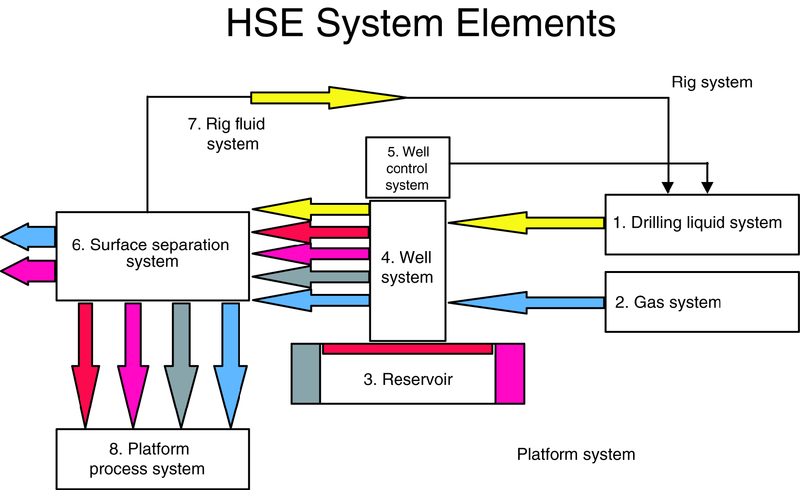
\includegraphics[scale=1.6]{Figs/Fig17.png}
		\caption{Hệ thống phân tích HSE\cite{HSE}}
	\end{figure}\newline
	\textbf{Môi trường:}\\
	Hệ thống khoan dưới cân bằng là một hệ kín. Khi kết hợp hệ thống bơm ép mùn khoan với hệ thống lọc mùn khoan, những vỉa chứa lưu huỳnh có thể được khoan một cách an toàn. Áp suất và lưu lượng được giữ ở mức nhỏ nhất có thể để hạn chế chất đọc hại rò rỉ ra môi trường. Trong những vỉa chứa nhiều mối nguy hiểm, tối ưu hóa sản lượng không phải là mục đích quan trọng nhất, thay vào đó việc phân tích mối nguy được thực hiện, vấn đề an toàn và môi trường được ưu tiên hàng đầu. Well test có thể được thực hiện trong quá trình khoan để có thể lấy được những thông tin cần thiết. Trong những giếng đã khai thác, một lượng lớn khí được đưa đi đốt, việc thu hồi lượng khí này sẽ mang lại nhiều lợi ích cho môi trường và kinh tế.\\
	\newpage
	\textbf{An toàn:}\\
	Bên cạnh việc phân tích mối nguy, cần phải thực hiện tập huấn cho những trường hợp đăc biệt kể cả việc phải hủy giếng. Ngược lai, việc hủy giếng là việc đâu tiên cần phải tránh để có thể giảm được những thiệt hại về kinh tế. Làm việc trên những giếng sống luôn luôn có những mối nguy hiểm cận kề, quá trình tập huấn tốt sẽ giảm thiểu tối đa những tai nạn có thể xảy ra.
\subsection{Candidates selection}
	Hầu hết các giếng đều có thể sử dụng phương pháp khoan dưới cân bằng, nhưng một số giếng chưa thể áp dụng phương pháp này vì những vấn đề liên quan tới tính chất địa chất và độ ổn định của đất đá trong vỉa. Với một số vỉa có những điều kiện không thuận lợi như áp suất, nhiệt độ nằm ở mức rất cao, những công nghệ hiện tại vẫn chưa thể đảm bảo được vấn đề an toàn và môi trường trong quá trình khoan vì vậy cũng không được áp dụng phương pháp khoan dưới cân bằng\cite{guo2002gas}. \\
	Việc lựa chọn những giếng có khả năng khoan bằng phương pháp khoan dưới cân bằng không chỉ phụ thuộc vào những lợi ích mà phương pháp này mang lại mà còn phải xem xét những yếu tố bên ngoài. Việc lựa chọn này cực kì quan trọng cho quá trình vận hành khoan có thể diễn ra thuận lợi nhất có thể. Tất nhiên không chỉ dựa vào phần đánh giá vỉa mà còn phải dựa trên quá trình thiết kế giếng, những nguy hiểm về mặt cơ khí và lợi ích về kinh tế. Tất cả những yếu tố đó cần được xem xét một cách cẩn thận khi lựa chọn phương pháp khoan dưới cân bằng cho giếng khoan.\\
	Những điều kiện sau mang lại lợi ích khi áp dụng khoan dưới cân bằng:
	\begin{itemize}
		\item Vỉa bị hư hại trong quá trình khoan hoặc hoàn thiện giếng, hệ số skin thường lớn hơn 5
		\item Vỉa có xu hướng ``sticking'' do chênh áp\newline
		\item Vỉa có những tầng dễ bị xâm nhập bởi dung dịch trong quá trình khoan hoặc hoàn thiện giếng
		\item Vỉa có những vết nứt nẻ kích thước lớn
		\item Vỉa có độ thấm thấp
		\item Vỉa có mức độ bất đồng nhất cao hoặc mức độ phân lớp lớn
		\item Dung dịch vỉa nhậy cảm
		\item Tốc độ khoan thấp khi sử dụng phương pháp khoan trên cân bằng.
	\end{itemize}
	Ngược lại khi vỉa có những tính chất sau, phương pháp khoan dưới cân bằng sẽ không được áp dụng:
	\begin{itemize}
		\item Phương pháp khoan truyền thống mang lại lợi ích kinh tế lớn
		\item Tốc độ khoan lớn (ROP$\geq$1,000 ft/day)
		\item Những vỉa có độ thấm cực lớn hoặc cực nhỏ
		\item Vỉa có độ cố kết thấp
		\item Những giếng có độ ổn định thành hệ thấp
		\item Vỉa gồm nhiều tầng mỏng nhỏ nằm rải rác, chế độ áp suất của mỗi tầng khác nhau
		\item Vỉa có sự xen kẻ giữa các lớp sét nén và đá sét.
	\end{itemize}
\subsection{Kiểm soát áp suất trong khi khoan (MPD)}
	MPD\cite{rehm2013managed} là quá trình kiểm soát áp suất trong khoảng không vành xuyến của giếng khoan. Mục đích để biết được chính xác áp suất giới hạn của môi trường và kiểm soát áp suất thủy lực trên bề mặt. \\
	MPD trong khoan dưới cân bằng\cite{engevik2007risk} cho kiểm soát áp suất chuẩn xác hơn so với các phương pháp kiểm soát truyền thống và thích hợp cho những tâng vỉa mỏng hẹp, những giếng có thành hệ nứt nẻ hoặc không ổn định. \\
	MPD mang lại một số ưu điểm:
	\begin{itemize}
		\item Giảm chi phí chống ống
		\item Giảm chi phi dung dịch khoan
		\item Giảm nonproductive time
		\item Nâng cao mức độ kiểm soát giếng
		\item Kiểm soát lưu lượng khí từ vỉa
		\item Tối thiểu mất mát dung dịch và kẹt cần
		\item Tăng tốc độ khoan
		\item Giảm dung dịch xâm nhập vào thành hệ và nứt nẻ
		\item Giảm thời giam khoan
		\item Tăng tuổi thọ choòng khoan.
	\end{itemize}
	\subsubsection{Vận hành MPD}
		Có hai cách tiến hành vận hành chính:
		\begin{enumerate}
			\item \textbf{Reactive} Dùng những thiết bị, chương trình khoan theo phương pháp truyền thống cho MPD
			\item \textbf{Proactive} Thiết kế chương trình khoan đặc biệt, sử dụng những thiết bị công nghệ cao để có thể tận dụng tối ưu những lợi ích của MPD.
		\end{enumerate}
		Ngoài hai phương pháp vận hành trên còn có những phương pháp vận hành khác được áp dụng cho kiểm soát áp suất khi khoan trên biển:
		\begin{itemize}
			\item Constant bottom-hole pressure (Khoan với áp suất đáy giếng ổn định)
			\begin{itemize}
				\item[-] Continuous circulation system (CCS), dynamic annular pressure control (DAPC), dung dịch khoan tỉ trọng thấp, hệ thống tuần hoàn dung dịch thứ cấp thay đổi tỉ trọng dung dịch khoan
			\end{itemize}
			\item Pressurized mud cap drilling (PMCD)
			\begin{itemize}
				\item[-] Low riser return system (LRRS)
			\end{itemize}
			\item Dual gradient (Khoan hai tỉ trọng)
			\begin{itemize}
				\item[-] Gas lift in riser, equivalent circulating density reduction tool (ECDRT), hệ thống tuần hoàn thứ cấp
			\end{itemize}
			\item HSE hoặc kiểm soát dòng hồi dung dịch.
		\end{itemize}
		Trong đó khoan với áp suất đáy giếng ổn định, PMCD và HSE là ba phương pháp được sử dụng nhiều nhất.
		\subsubsection{Thiết bị kiểm soát}
		Thiết bị bề mặt sử dụng trong vận hành MPD bao gồm bộ kiểm soát khoan xoay và một số các thiết bị dưới đây:
		\begin{itemize}
			\item Đường tiết lưu kiểm soát đối áp trong quá trình vận hành khoan, có thể được kiểm soát bằng tay hoặc tự động
			\item Hệ thống kiểm soát dòng vào không mong muốn
		\end{itemize} 
		Thiết bị kiểm soát áp suất (RCD), kiểm soát đông năng khoan xoay, áp suất khoảng không vành xuyến trong quá trình khoan. Có ba loại thiết bị kiểm soát khoan xoay thường dùng:
		\begin{itemize}
			\item Hệ thống bị động, phụ thuộc vào ma sát giữa cần khoan, rotating pack-off và áp suất tác động lên màng chắn
			\item Hệ thống chủ động, sử dụng hệ thống thủy lực
			\item Hệ thống ghép, sử dụng kết hợp hệ thống chủ động và hệ thống bị động.
		\end{itemize}
		Thiết bị kiểm soát khoan xoay gồm ba bộ phận chính:
		\begin{itemize}
			\item Thân thiết bị với với mặt bích kết nối dòng ra
			\item Bộ đỡ với Stripper Rubber dùng để kéo thả cần khoan và tool joints
			\item Kẹp và chốt để kết nối bảo vệ bộ đỡ, stripper rubber với bệ đỡ.
		\end{itemize}
		Ngoài ra, còn có một số thiết bị phụ như hệ thống loại bỏ tĩnh điện, bơm, hệ thống nhận và lưu trữ dữ liệu.
%\newpage
\section{Kiểm soát thông số trong quá trình khoan dưới cân bằng}
\subsection{Các thống số trong quá trình khoan dưới cân bằng}
Công thức tính áp suất đáy giếng (BHP):
\begin{equation}
p_{bh} = p_{hyd}+p_{af}+p_{c}
\end{equation}
Trong đó:
\begin{itemize}
		\item[-] $p_{bh}$ là áp suất đáy giếng
		\item[-] $p_{hyd}$ là áp suất cột áp thuỷ tĩnh
		\item[-] $p_{af}$ là tổn thất áp suất trong khoảng không vành xuyến
		\item[-] $p_{c}$ là áp suất van điều chỉnh tại bề mặt.
\end{itemize}
Dòng chảy từ vỉa vào giếng được xác định bằng nhiều mô hình tương ứng với các chế độ dòng khác nhau: ổn định (steady-state flow), giả ổn định (pseudo-steady-state flow) và chuyển tiếp (transient flow).\\

Từ mô hình cơ bản và đơn giản của \textit{Dake 1978} tương quan dòng vào được tính bởi công thức:
\begin{equation}
q_{res} = max [0, k_{pi}.(p_{pore}-p_{bh})]
\end{equation}
Trong đó:
\begin{itemize}
	\item $q_{res}$ là lưu lượng dòng vào vỉa
	\item $p_{pore}$ là áp suất trung bình vỉa
	\item $k_{pi}$ là chỉ số khai thác của vỉa (production index)
\end{itemize}
 Những thông số chúng ta có thể kiểm soát được là\cite{pedersen2015supervisory}:
\begin{enumerate}
 	\item[] Bottom Hole Pressure $p_{bh}$
 	\item[] Casing-shoe pressure $p_{cs}$
 	\item[] Choke-pressure $p_{choke}$
 	\item[] Standpipe pressure $p_{sp}$
 	\item[] Seperator pressure $p_{s}$
 	\item[] Pump volumetric flow $q_{p}$
 	\item[] Actual choke opening $z_{choke}$
\end{enumerate}
 Điều kiện biên:
\begin{displaymath}
p_{col}(bh) \leq p_{bh} \leq p_{pore}(bh)
\end{displaymath}
\begin{displaymath}
p_{col}(cs) \leq p_{cs} \leq p_{pore}(cs)
\end{displaymath}
\begin{displaymath}
p_{choke,min} \leq p_{choke} \leq p_{choke,max}
\end{displaymath}
\begin{displaymath}
p_{sp} \leq p_{sp,max}
\end{displaymath}
\begin{displaymath}
z_{c,min} \leq z_{c} \leq p_{c,max}
\end{displaymath}
 


\subsection{Ổn định thành hệ trong khoan dưới cân bằng}
Trong qua trình khoan dưới cân bằng, bởi vì áp suất thành hệ thường được giữ nhỏ hơn áp suất vỉa. Kết quả là trong quá trình khoan, các chất lưu từ vỉa có thể chảy vào giếng, được tuần hoàn lên trên bề mặt và được kiểm soát bởi các thiết bị bề măt. Tuy vậy, bởi vì áp suất đáy giếng nhỏ hơn áp suất vỉa thường gây ra những nguy hiểm đến tính ổn định của thành hệ.
\newline
Sự ổn định thành hệ trong quá trình khoan dưới cân bằng thường\cite{mclellan1999borehole} rất phức tạp và liên quan đến nhiều nhân tố trong đó áp suất cột chất lỏng và độ bền cơ học của thành hệ đất đá xung quanh là rất quan trọng. Trong khoan dưới cân bằng ta có thể chia làm hai trường hợp:
\begin{enumerate}
	\item[] Trường hợp 1
	\begin{equation}
	MW<P_{p}<P_{f}
	\end{equation}
	\item[] Trường hợp 2
	\begin{equation}
	P_{p}>MW>P_{f}
	\end{equation}
\end{enumerate}
\clearpage
\begin{figure}
\centering
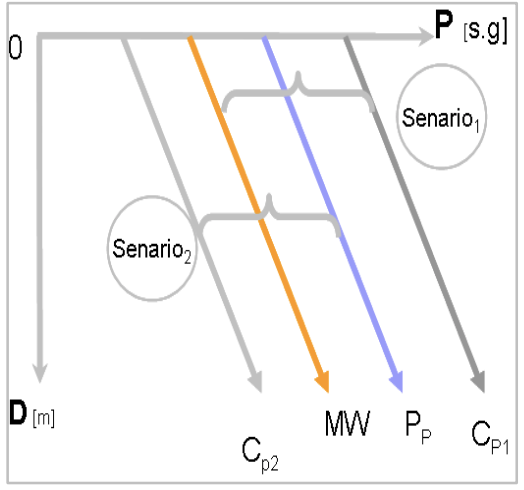
\includegraphics[scale=1]{Fig5_10}
\caption{Hai trường hợp áp suất trong khoan dưới cân bằng\cite{guo2002gas}}
\end{figure}
Trong cả hai trường hợp, chúng ta chỉ có thể kiểm soát áp suất của cột dung dịch khoan, hai thông so $P_{p}$ và $P_{f}$ không kiểm soát được. Có rất nhiều mô hình được áp dụng để đánh giá sự ổn định thành hệ trong quá trình khoan. Mô hình đơn giản nhất được dùng đó là tính toán trường ứng suất tại đáy giếng trong trường hợp giả sử đất đá xung quanh nằm trong miền đàn hồi tuyến tính, sau đó so sánh với các tiêu chí độ bền cơ học của đất đá và đưa ra mô hình chính xác. Ngoài ra, dựa trên việc phân tích mô hình địa cơ học của đất đá xung quanh giếng khoan, chúng ta có thể dự báo được sự ổn định của thành hệ.

\subsection{Thiết bị trong khoan dưới cân bằng}
%\clearpage
%\begin{figure}[h]
%\centering
%\includegraphics[width = 16cm, height = 10cm]{fig5_2.png}
%\caption{Hệ thống tuần hoàn kín trong quá trình khoan dưới cân bằng}
%\end{figure}
Quá trình khoan dưới cân bằng, ngoài yêu cầu các thiết bị như trong quá trình khoan truyền thống như:
\begin{itemize}
	\item Hệ thống cung cấp năng lượng
	\item Hệ thống tuần hoàn dung dịch
	\item Hệ thống nâng hạ
	\item Hệ thống xoay
	\item Hệ thống theo dõi các thông số khoan
	\item Hệ thống chống phun
	\item Hệ thống kiểm soát giếng
\end{itemize}
Yêu cầu về các thiết bị đặc biệt phục vụ công tác thi công khoan dưới cân bằng như:
\begin{enumerate}
	\item[] Thiết bị lấy mẫu địa chất
	\item[] Thiết bị kiểm soát áp suất (RCD)
	\item[] Bình tách bốn pha
	\item[] Thiết bị kiểm soát dòng 
	\item[] Thiết bị kiểm soát

\end{enumerate}
Duới đây là sơ đồ các thiết bị trong quá trình khoan dưới cân bằng.
%\clearpage
\begin{figure}[h]
\centering
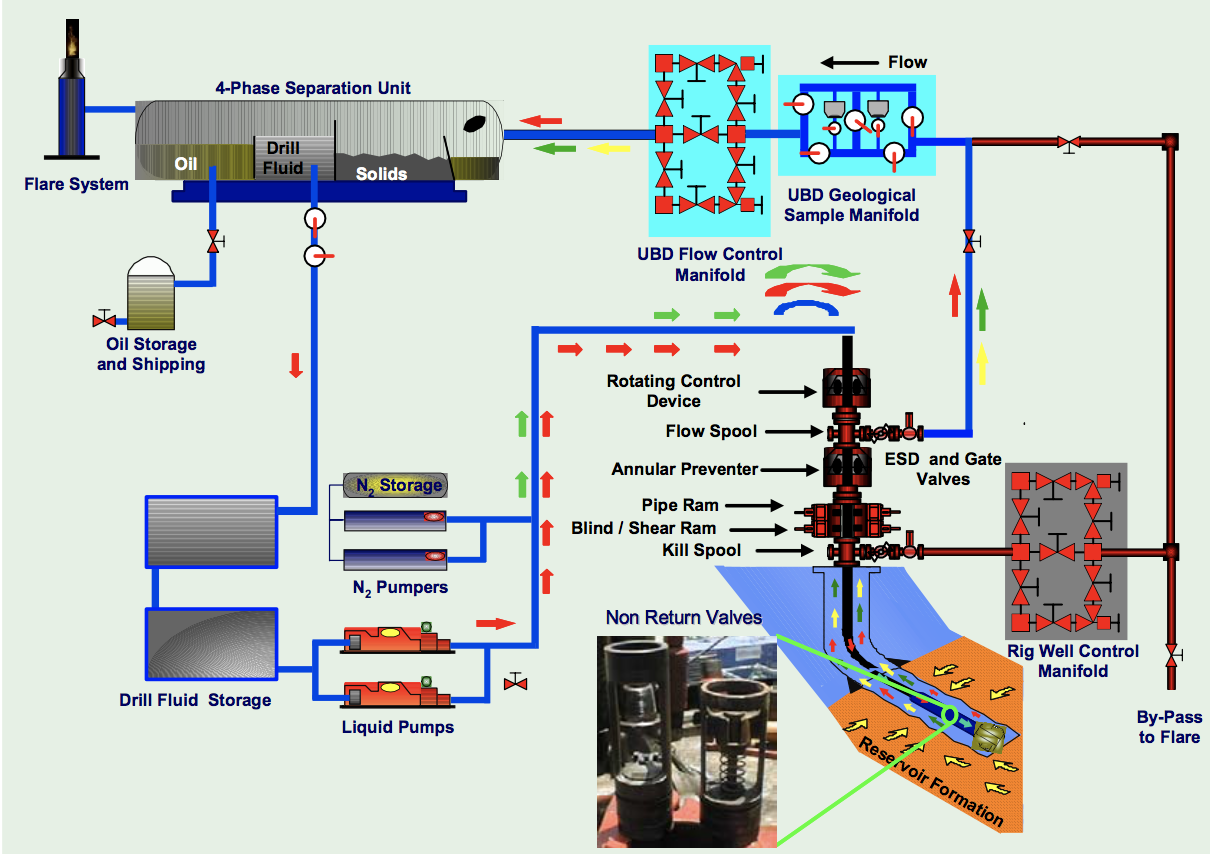
\includegraphics[scale = 0.6]{Fig5_8}
\caption{Sơ đồ thiết bị trong quá trình khoan dưới cân bằng\cite{ramalho2007changing}}
\end{figure}


\subsubsection{Thiết bị lấy mẫu địa chất}
Thiết bị lấy mẫu đia chất trong khoan dưới cân bằng là một ống thu gom áp suất lớn có thể chuyển hướng dòng chất lưu từ vỉa đến những thiết bị chứa đặc biệt mà ở đó dòng chất lưu đi qua được xử lý lọc chất rắn mà vẫn giữ áp suất ổn định.
Chức năng chính của thiết bị lấy mẫu này là đánh giá chất lượng của đá chứa trong vỉa.
Thiết bị này sử dụng GammaRay, Neutron Porosity, Neutron Density và Sonic Tools kết hợp với phương pháp đo trong quá trình khoan (LWD) để đánh giá chất lượng đá vỉa trong quá trình vận hành khoan dưới cân bằng (UBD).
%\clearpage
\begin{figure}
\centering
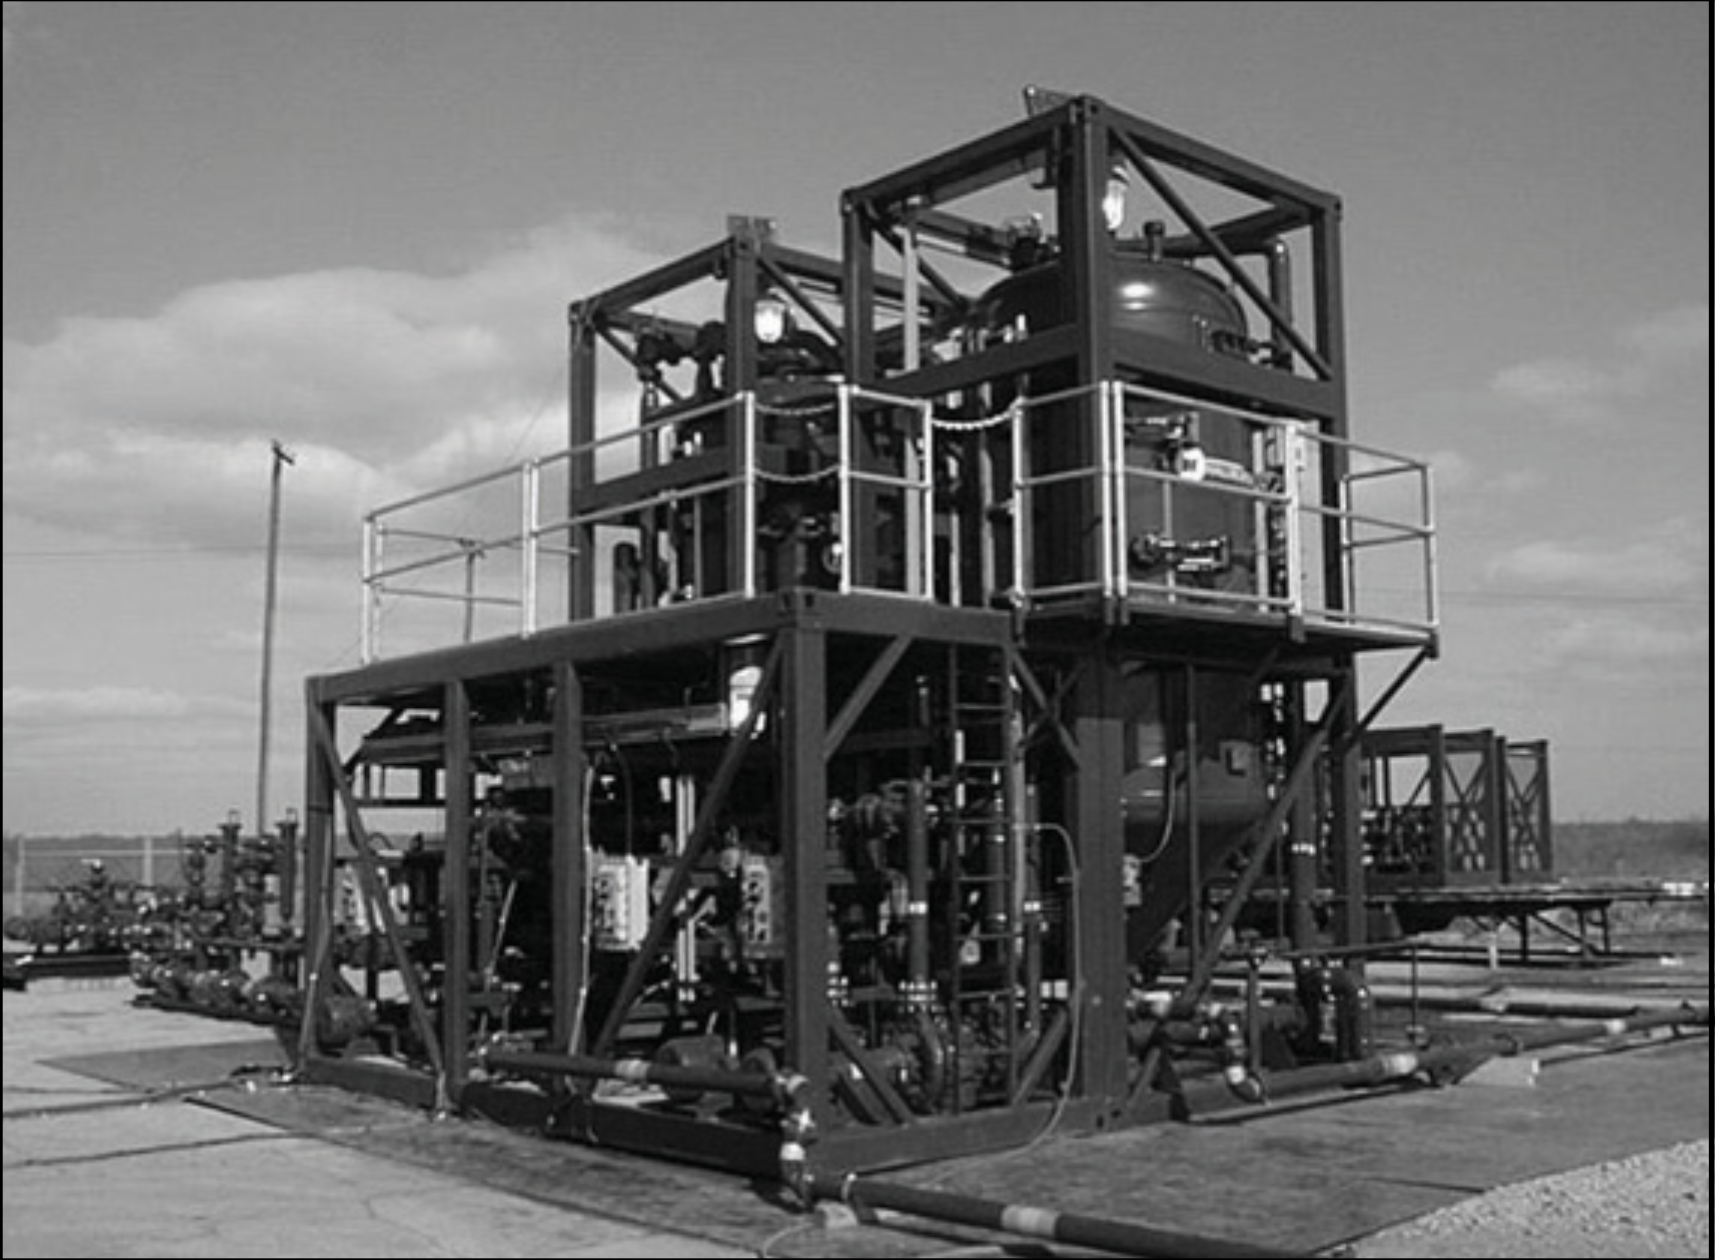
\includegraphics[scale =0.4]{Fig5_5}
\caption{Thiết bị lấy mẫu địa chất phục vụ khoan dưới cân bằng\cite{rehm2013underbalanced}}
\end{figure}

\subsubsection{Thiết bị kiểm soát áp suất RCD}
Khoan dưới cân bằng yêu cầu một vòng tuần hoàn kín cho hệ thống tuần hoàn dung dịch khoan. Chìa khoá để thực hiện điều này chính là thiết bị kiểm soát áp suất (RCD). Thiết bị này dùng để duy trì áp suất và điều chỉnh lượng dung dịch tuần hoàn trong hệ thống.
Thiết bị RCD thường được gắn chung với thiết bị chống phun trào (BOP) nên cũng có thể gọi là thiết bị R-BOP.
\clearpage
\begin{figure}
\centering
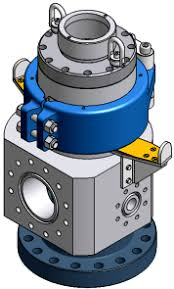
\includegraphics[scale = 1]{Fig5_9}
\caption{Thiết bị kiểm soát áp suất RCD\cite{nikoofard2016control}}
\end{figure}

\subsubsection{Bình tách bốn pha}
Có hai loại bình tách được thiết kế để dùng cho quá trình khoan dưới cân bằng đó là bình tách đứng và bình tách ngang.
Trong trường hợp tách khí từ hỗn hợp khí và chất lỏng, bình tách đứng được dùng hiệu quả nhất.
Trong trường hợp hỗn hợp chất lưu lỏng với các tỷ trọng khácn nhau, bình tách ngang là tối ưu nhất.
Thiết kế bình tách cho khoan dưới cân bằng đòi phụ thuộc vào thiết kế giếng khoan và các thông số khác như:
\begin{itemize}
	\item Loại dung dịch khoan
	\item Lưu lượng bơm
	\item Lưu lương khai thác kỳ vọng
	\item Tính chất chất lưu và chế độ dòng chảy trong vỉa
	\item Một số thông số khác như: bán kính lỗ khoan, chiều dài giếng, độ dày vỉa và các thông số môi trường.
\end{itemize}
%\clearpage
\begin{figure}[h]
	\centering
	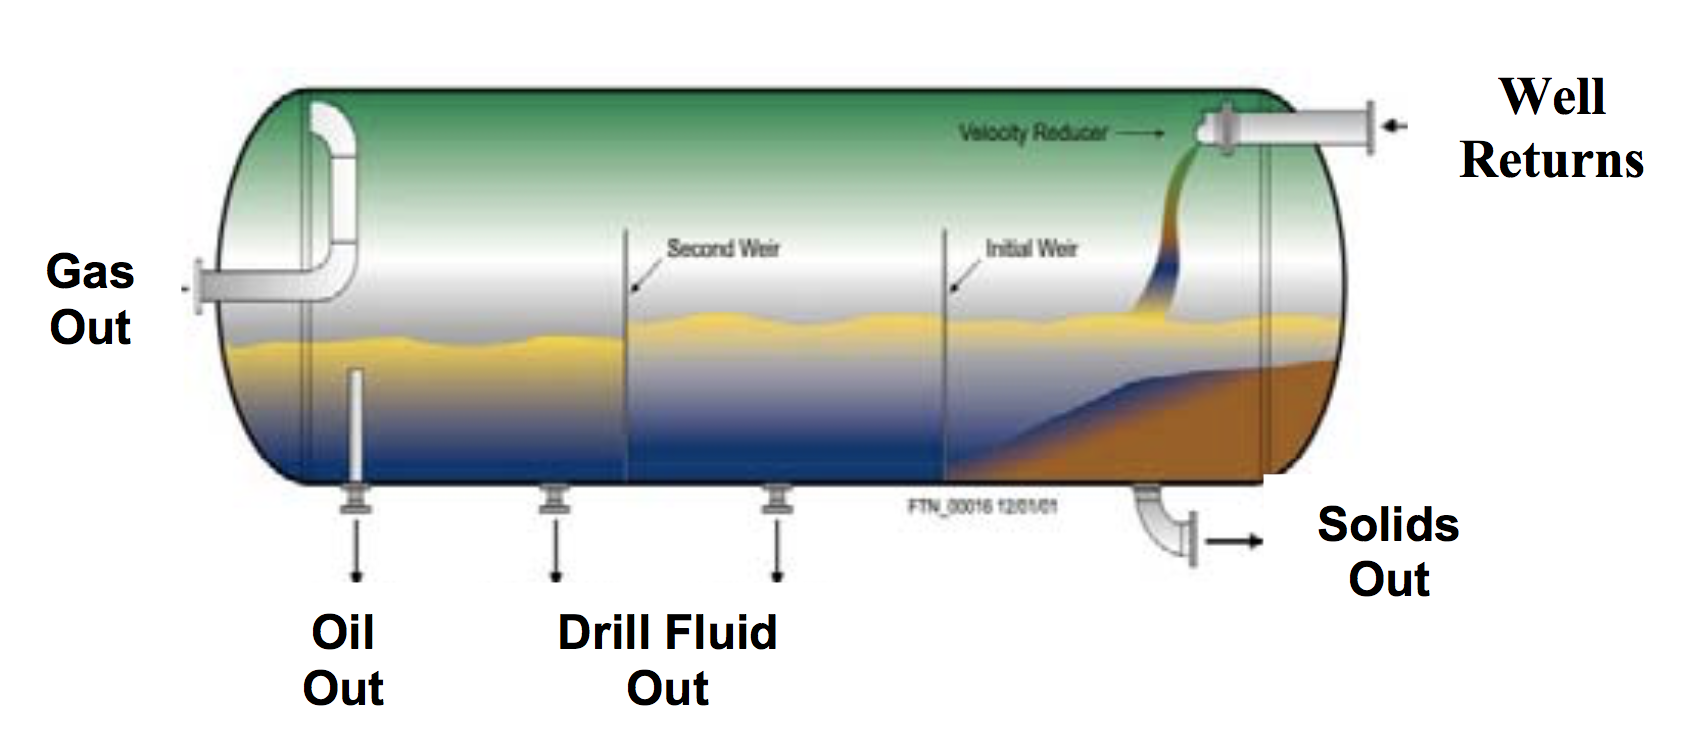
\includegraphics[width = 16cm ,height = 7cm]{Fig5_4.png}
	\caption{Bình tách bốn pha trong quá trình UBD\cite{ramalho2007changing}}
\end{figure}
Chức năng cần thiết của bình tách\cite{ramalho2007changing}:
\begin{itemize}
	\item Tách hỗn hợp dầu, khí, nước và chất rắn theo những dòng khác nhau.
	\item Có khả năng đo các thống số lưu lượng dòng để giúp tính toán dòng sản phẩm của một giếng, hay vùng mỏ hoặc tính toán các thông số để xác định IPR (Inflow Relationship Performance).
\end{itemize}
Trong phần lớn các giếng áp dụng kỹ thuật khoan dưới cân bằng, bình tách ngang bốn pha được sử dụng nhiều nhất và rộng rãi nhất.
\section{Kết luận và kiến nghị}
\subsection{Kết luận}
Trong quá trình khoan, thiết kế lựa chọn phương pháp khoan rất quan trọng. Khi phương pháp khoan dưới cân bằng được lựa chọn để áp dụng cho một giếng khoan, quá trình tìm hiểu các tính chất địa chất, tính toán lợi ích về mặt kinh tế được triển khai cẩn thận để có thể xác định những thông số cho việc lựa chọn các kĩ thuật khoan trong khoan dưới cân bằng. Những kĩ thuật thông dụng thường được sử dụng nhiều nhất trong phương pháp khoan dưới cân bằng là:
	\begin{itemize}
		\item Kĩ thuật khoan bằng khí
		\item Flow drilling (Drilling mud)
		\item Kĩ thuật khoan bằng khí mù
		\item Kĩ thuật khoan bằng bọt
		\item Gaseated mud (Gasified liquid drilling).
	\end{itemize}
Dòng và áp suất là hai thông số đặc biệt quan trọng cần kiểm soát để có thể thành công trong quá trình vận hành khoan dưới cân bằng. Áp suất trong giếng, mức trong bình tách và áp suất trong bình tách được điều khiển bằng tay thông qua các thiết bị như bơm, choke và van bình tách. Bằng cách hạn chế lưu lượng và mức độ thay đổi của dòng vào từ trong vỉa, khoảng thời gian ``chết'' (NPT) được giảm đi khá nhiều, đồng thời tăng hệ số an toàn trong khi khoan và giảm được mức độ ảnh hưởng tới môi trường.
\subsection{Kiến nghị}
Quá trình điều khiển các thông số phải dựa trên mô hình điều khiển dự đoán (Model Predictive Control, MPC) và nhiều phần mềm mà nhóm chưa có điều kiện được tiếp xúc. Vì vậy, khá nhiều thông số chỉ được xem xét trên mặt lý thuyết. Nếu có cơ hội nhóm hy vọng có thể được tạo điều kiện để kiểm tra kết quả điều khiển trên phần mềm thực tế.
%\subsection{Quá trình vận hành}
%\clearpage
%\begin{figure}[h]
%	\centering
%	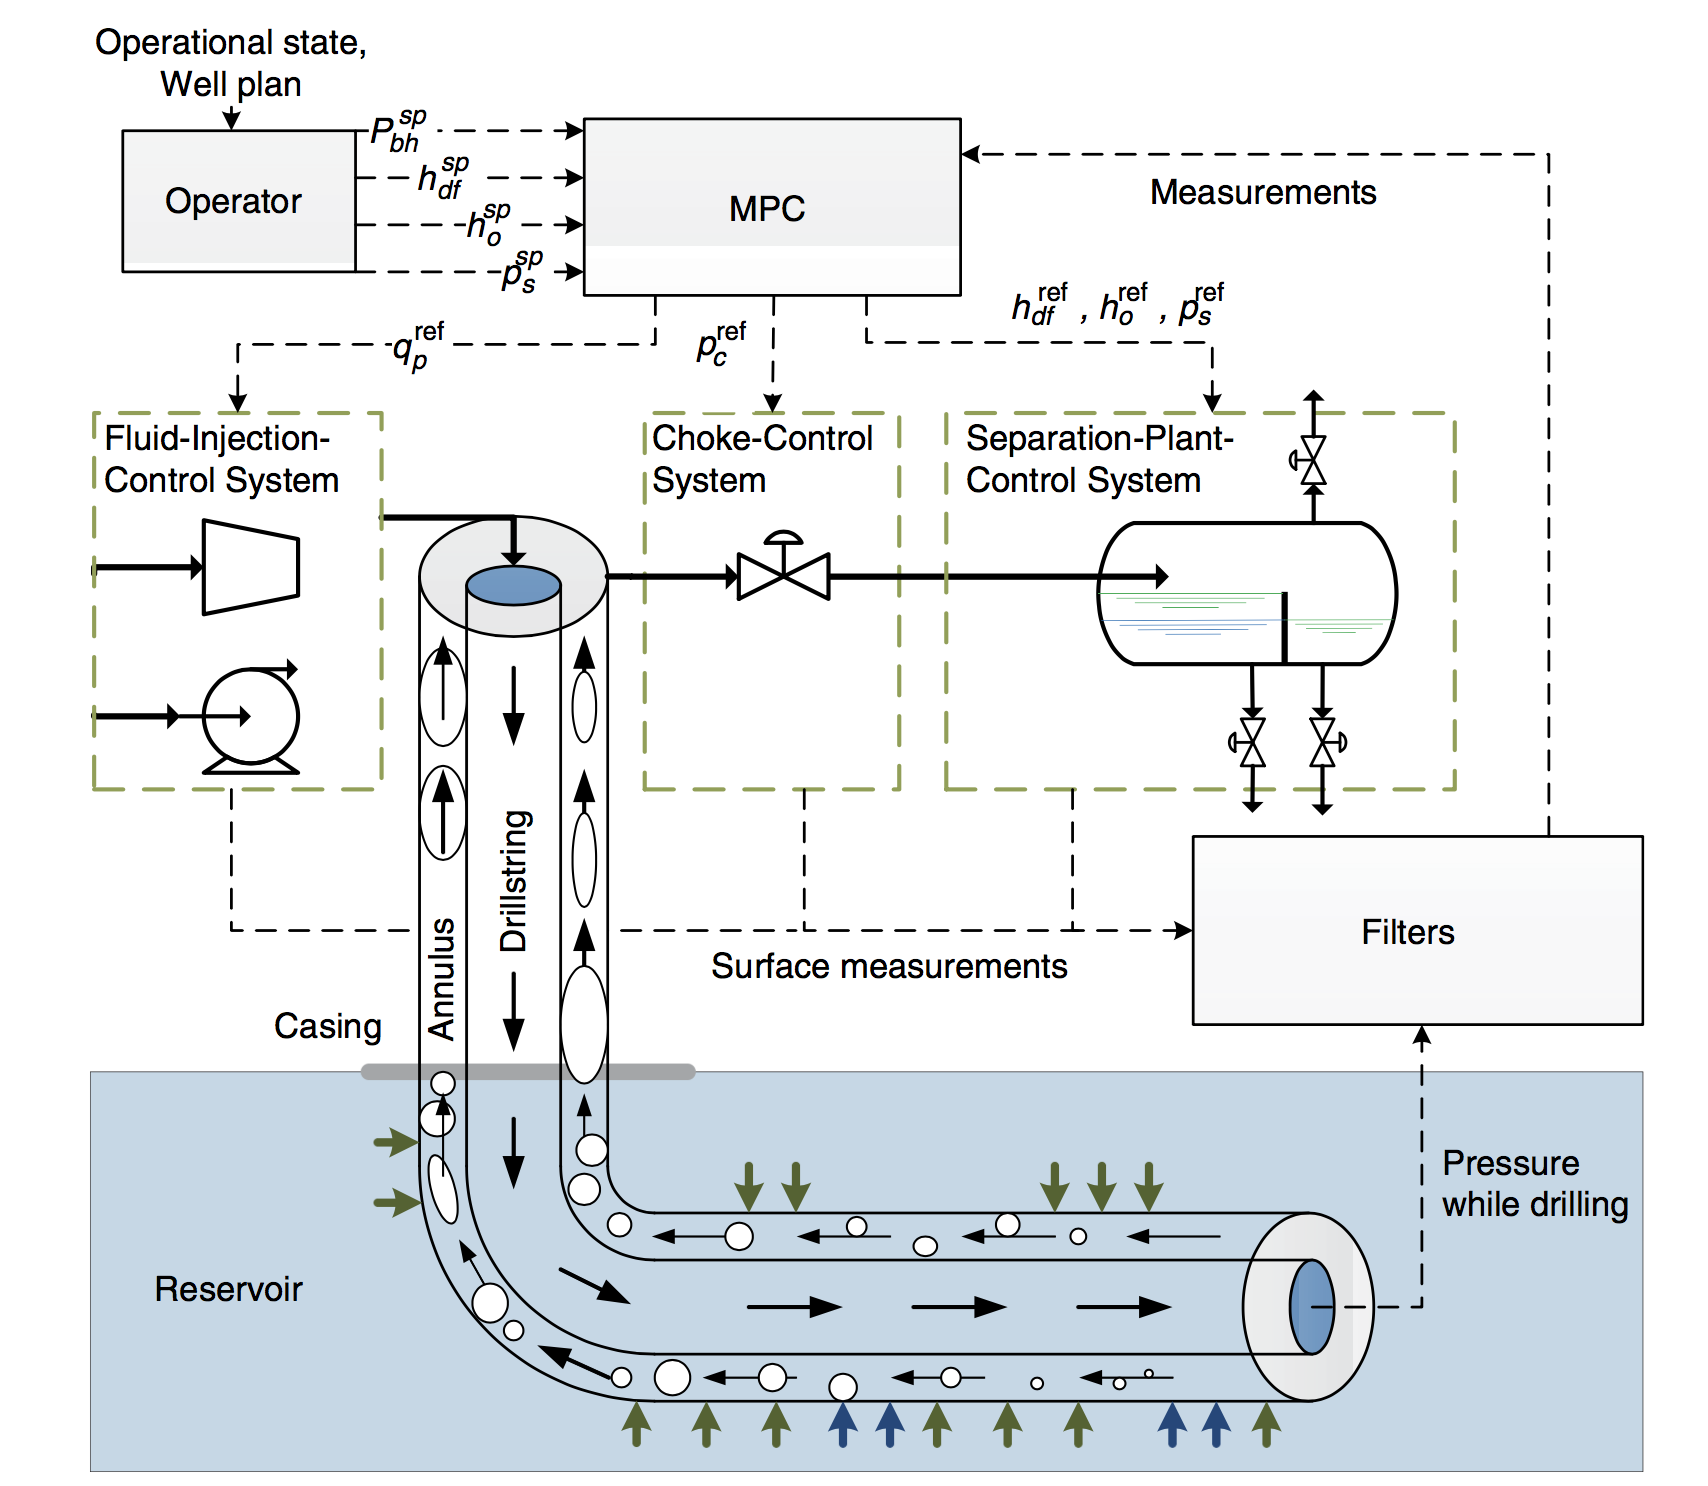
\includegraphics[width = 16 cm, height =13 cm]{Fig5_3.png}
%	\caption{Simple sketch of the well and topside equipment.}
%\end{figure}
%Quy trình vận hành khoan đưới
\newpage
\bibliographystyle{ieeetr}
\bibliography{Ref}
\end{document}